% Main file -- Thematic Paper plan, Traditional Format (PR07284).
% Migrated from muthesis2021 to muthesis2026 on 2026-08-06.
\documentclass{muthesis2026}
\setcounter{tocdepth}{2}   % sections + subsections in the TOC (2026 class defaults to chapters only)
\thematicplan   % 2026: replaces the hand-edited "Thematic Paper" strings in the old .cls
\usepackage[numbers]{natbib}
\setcounter{secnumdepth}{4} % make subsubsection have numberings
\usepackage{graphicx}
\graphicspath{{figures/}}
\usepackage{latexsym}
\usepackage{amsmath}
\usepackage{amsthm}
\usepackage{url}
\usepackage{xurl}
\usepackage{textcomp}
\usepackage{longtable}
\usepackage{caption,setspace}
\usepackage[utf8]{inputenc}
\usepackage[T1]{fontenc}
%\usepackage{geometry}
\usepackage{pdflscape}   % For landscape pages
\usepackage{array}       % For paragraph columns
\usepackage{booktabs}
\usepackage{tabularx}
\usepackage{makecell}
\usepackage{multirow}
\usepackage[table,xcdraw]{xcolor}
\usepackage{listings}
\lstset{
  basicstyle=\ttfamily\small,
  breaklines=true,      % Enables automatic line breaking
  columns=fullflexible,
  breakatwhitespace=false
}
\usepackage{float}       % was declared inside preamble.tex in the Aug 2026 source
\captionsetup{font={stretch=1.5}} % make the table,figure captions also have 1.5 linespacing
\usepackage[flushleft]{threeparttable}
\usepackage[hidelinks]{hyperref}
\makeatletter
\renewcommand{\@dotsep}{10000} % set distance between dots to make it disappear in the table of contents
\setlength{\@fptop}{0pt}
\setlength{\@fpbot}{0pt plus 1fil}
\makeatother
% title -- nouns and stressed words should begin with a capital
\title{A COMPARATIVE STUDY OF OPEN-SOURCE BREACH AND ATTACK SIMULATION TOOLS}
\author{THANAWUT UDOMSILP}
\candidate{Thanawut Udomsilp} % your name (without title)

\candidatetitle{Mr.\ } % Mr.\ Miss.\ or Ms.\

\degree{MSc} % MSc or PhD

\subject{CYBER SECURITY AND INFORMATION ASSURANCE} % subject area

\submissionyear{2026} % default is current year

%\isbn{974-04-xxxx-x} % remember to replace the x's when you know the number

% information for page i (advisory committee)


\majoradvisor{Vasaka Visootiviseth} % name of supervisor (without title)
\majoradvisortitle{Assoc.~Prof.~} % Dr.~ or Asst.~Prof.~ or Assoc.~Prof.~ or Prof.~
\majoradvisorletters{Ph.D.} % Ph.D. or Dr.rer.nat.
\majoradvisorsubject{Computer Engineer} % subject in which advisor obtained last degree

\coadvisor{Ittipon Rassameeroj} % name of co-advisor
\coadvisortitle{Dr.~} % title of co-advisor
\coadvisorletters{Ph.D.} % Ph.D. or Dr.rer.nat.
%\coadvisorstatus{Major advisor} % default is Co-advisor
\coadvisorsubject{Computer Science} % subject in which co-advisor obtained last degree

\coadvisorII{Dolvara Guna-Tilaka}
\coadvisorIItitle{Assoc.~Prof.~}
\coadvisorIIletters{Ph.D.}
\coadvisorIIsubject{Computer Science}

\programchair{Vasaka Visootiviseth} % chair of your degree program
% DELIBERATE OVERRIDE (re-applied 2026-09-14; was lost when the template
% preamble was merged in). muthesis2026.cls line ~513 unconditionally typesets
%     \@programchairqual~(\@subject)
% which force-appends the STUDENT's programme subject and prints
% "Ph.D. (CYBER SECURITY AND INFORMATION ASSURANCE)" -- wrong; the Program
% Director's degree is Ph.D. (Computer Engineer). \@gobblefour swallows the
% four appended tokens. The class file is left unmodified.
% If muthesis2026.cls is ever updated and the auto-append is removed, delete
% \@gobblefour or it will eat the following four tokens.
\makeatletter
\programchairqual{Ph.D. (Computer Engineer)\@gobblefour}
\makeatother
\faculty{Information and Communication Technology}

% 2026 CHANGE: \GSDqual is no longer typeset. The dean's qualification must be
% written inside \graduatestudiesdean, using \\ for the second line.
\graduatestudiesdean{Prof.~Dr.~Chartchalerm Isarankura-Na-Ayudhya,\\Ph.D. (Medical Technology)}
%\GSDstatus{Acting} % in case the dean is away and you need `Acting Dean' on the form

% information for page ii (exam committee)

\submissiondate{Month Day, Year} % date of submission -- FILL IN BEFORE SUBMISSION

\chair{Chair Name}
\chairqual{Ph.D.}
\chairsubject{Computer Science}

% NOTE: muthesis2026 no longer substitutes \memberI--\memberIV on the exam
% committee page; it always lists chair, major advisor, then co-advisors.
%\memberI{}
%\memberIqual{}
%\memberII{}
%\memberIIqual{}
%\memberIII{}
%\memberIIIqual{}
%\memberIV{}
%\memberIVqual{}

\facultydean{Pattanasak Mongkolwat}
% 2026 CHANGE: split into \FDqual + the new \FDsubject.
% Was: \FDqual{Ph.D. (Computer Science)}
\FDqual{Ph.D.}
\FDsubject{Computer Science}
%\FDstatus{Acting}

% information for page iv (ABSTRACT)

\candidatenumber{6738220 ITCY/M}
%\major{} % major (not necessary if the same as subject)
\keywords{Breach and Attack Simulation (BAS) / MITRE ATT\&CK} % 1st line of keywords
\keywordsII{framework/ Open-source security tools} % 2nd line of keywords
\keywordsIII{Experimental testing / Comparative analysis} % 3rd line of keywords

% information for page v (THAI ABSTRACT)
% NOTE: muthesis2026 dropped \thaiabstract entirely (the Thai font dbtt is gone;
% the class now uses cmr10). Produce the Thai abstract in MS Word, as before.
\thaisubject{ชื่อสาขาภาษาไทย} % thai name of degree subject
\thaititle{ชื่อเรื่องภาษาไทย} % title in thai -- FILL IN
\thaicandidate{นายธนาวุฒิ อุดมศิลป์} % your name in thai
\thaimajoradvisor{รศ. ดร. วสกา วิสุทธิวิเศษ} % Thai name of advisor
%\thaicoadvisor{}
%\thaicoadvisorII{}

% information for Biography

\dateofbirth{26 October 1988} % your date of birth
\placeofbirth{Chumphon, Thailand} % province and country of birth
\firstdegreeinstitution{Kasem Bundit University} % where you did your first degree
\firstdegreeyears{2007--2011} % years for 1st degree
\firstdegree{Bachelor of Engineering} % default is Bachelor of Science
\firstdegreemajor{Computer Engineer} % first degree major
%\longfirstdegree % necessary if you want the subject on the next line
%\preinstitution{}
%\preinstitutionLnII{}
%\preinstitutionII{}
%\preinstitutionIILnII{}
\years{2024--2026} % years taken to do your present degree
\postinstitution{Mahidol University}
%\postinstitutionLnII{}
%\scholarship{}
%\scholarshipLnII{}
%\scholarshipLnIII{}
%\scholarshipII{}
%\scholarshipIILnII{}
%\scholarshipIILnIII{}

% 2026 NEW: the Biography page now prints RESEARCH GRANTS and
% PUBLICATION/PRESENTATION rows. Leaving them empty prints "-".
%\researchgrants{Grant name, funding agency, year}
%\researchgrantsLnII{}
%\researchgrantsLnIII{}
%\publications{Author(s). Title. Journal. Year;Vol(Issue):Pages.}
%\publicationsLnII{}
%\publicationsLnIII{}

\position{Assistance Vice President - Cyber Security Operation and Defense Center} % present position
\workplace{CIMB Thai Bank} % location
\workplaceLnII{Bangkok, Thailand} % second line of location
%\homeaddress{} % your home address if you do not have a position
%\homeaddressLnII{}
%\homeaddressLnIII{}
\email{thanawutu@icloud.com} % email at which you can be contacted after you leave

\begin{document}
\maketitle
\linespacing{1.5}
\acknowledgements{
This thematic paper could not have been completed without the invaluable support, guidance, and encouragement of many individuals.

First and foremost, I would like to express my deepest gratitude to Assoc. Prof. Vasaka Visootiviseth, Ph.D., my major advisor, for his continuous guidance, insightful suggestions, and patient supervision throughout every stage of this research. His expertise and encouragement have been instrumental in shaping both the methodology and the analytical framework of this study.

I am also grateful to all faculty members and administrative staff of the M.Sc. in Cyber Security and Information Assurance Program, Mahidol University, for their academic advice, resources, and administrative support throughout my studies.

Special thanks are extended to all cybersecurity professionals, colleagues, and respondents who generously shared their time, expertise, and perspectives, contributing valuable input to the comparative analysis and evaluation framework used in this research.

Finally, I am deeply thankful to my family and friends for their understanding, patience, and unwavering encouragement. Their continuous support has been my greatest strength throughout this academic journey.
}
% --- Abstract Section ---
% 2026 CHANGE: \abstract now takes ONE argument (was two in muthesis2021).
% The old second argument produced the "IMPLICATION OF THE THESIS" block,
% which no longer exists in muthesis2026. It has been removed.
\abstract{%
\linespacing{1.2} % change the linespacing to fit the abstract in the allotted space
While organizations invest heavily in layered defensive measures, validating the true efficacy of these controls against evolving threats remains a significant challenge. Breach and Attack Simulation (BAS) offers a solution by automating the emulation of adversarial tactics to proactively identify detection gaps. However, the high licensing costs of commercial BAS platforms often exclude budget-constrained organizations, and there is currently a lack of systematic, empirical data comparing viable open-source alternatives.

This research addresses this gap by applying the MITRE ATT\&CK framework to design, execute, and analyze real-world attack simulations. We conducted a comparative experimental analysis of three open-source BAS tools—MITRE Caldera, Infection Monkey, and Atomic Red Team—using the ATT\&CK framework to map adversarial tactics, techniques, and procedures across all test scenarios. The tools were evaluated against six proposed metrics: usability and deployment complexity, threat intelligence alignment and maintenance, scenario coverage and execution reliability, operational performance and output quality, framework extensibility and custom scenario creation, and community health and project maturity. All simulations were performed in a controlled laboratory environment designed to model real operational constraints.

The findings are based on actual experimental outcomes, with the performance of each tool visualized using radar charts. By aligning the evaluation process with MITRE ATT\&CK, this study provides evidence-based insights into the capabilities of open-source BAS tools, supporting organizations in advancing their security posture without incurring significant financial overhead.
}
 % point to english abstract.tex
% 2026: \thaiabstract was removed from the class. The Thai abstract is produced
% separately in MS Word, as before.

\tableofcontents
\listoftables
\listoffigures

% 2026: replaces the old abbrlist/symlist commands. Uncomment if needed.
%\listofabbreviations{
%\begin{tabbing}
%\hspace{3cm}\=\kill
%BAS \> Breach and Attack Simulation \\
%TTP \> Tactics, Techniques, and Procedures \\
%\end{tabbing}
%}
% PR07284 allows a flexible chapter structure for the thematic paper,
% at the discretion of the advisory committee. The five chapters below
% are carried over unchanged from the muthesis2021 version.
%CHAPTER 1 Introduction 
\chapter{Introduction}\label{chap:intro}
This chapter delineates the concept of Breach and Attack Simulation (BAS) and establishes its essential role in the testing of security defenses. Examines miter Caldera, Infection Monkey, and Atomic Red Team, specifically focusing on their architecture and capabilities. In conclusion, the chapter reviews earlier studies that have compared these tools to establish the existing state of knowledge.
% 1.1 Motivation
\section{Motivation}\label{sec:Motivation}
Cyber threats are growing rapidly in both volume and sophistication. Attacks now originate from both internal and external sources, traversing multiple channels such as social media, email, SMS, and internal systems\cite{verizon2024}. The widespread availability and ease of use of automated attack tools have lowered the entry barrier for malicious actors, making it easier to breach defenses, steal data, and deploy ransomware\cite{enisa2024}. Given this landscape, organizations must continually improve and validate their security postures.

Organizations often rely on a range of defensive measures to protect against these threats. These include human-centric controls like security awareness training for employees and proactive assessments such as penetration testing and Red Team exercises. They also deploy a vast array of technological defenses, including Intrusion Prevention Systems (IPS), Intrusion Detection Systems (IDS), Antivirus software, Network Firewalls, Web Application Firewalls (WAF), Endpoint Detection and Response (EDR), Network Detection and Response (NDR), and Data Loss Prevention (DLP) solutions\cite{nist80053}. However, even with these extensive tools and methodologies, it remains challenging to definitively assess an organization’s true security posture and its readiness for evolving sophisticated attacks\cite{mandiant2023}.

In response to this challenge, many organizations are adopting Breach and Attack Simulation (BAS), a proactive cybersecurity testing approach that automates the simulation of various cyberattacks to evaluate an organization’s defenses\cite{gartner_bas}. BAS tools simulate real-world attacks—such as malware infiltrations and phishing campaigns—and provide continuous visibility into vulnerabilities across endpoints, networks, and applications. Unlike traditional discrete vulnerability assessments and scans, BAS provides a continuous feedback loop, allowing security teams to quickly address weaknesses as they appear and stay ahead of evolving threats.

While commercial BAS tools are highly effective, their high cost often makes them inaccessible to small or budget-limited organizations. Fortunately, several free and open-source BAS tools have emerged, offering a viable alternative for organizations looking to improve their security posture without significant financial investment.

This research aims to evaluate and compare leading open-source BAS tools to provide a comprehensive, evidence-based guide for organizations. Potential candidates were initially identified by querying five independent AI assistants (Gemini, ChatGPT, Copilot, Claude, and DeepAI) to identify prominent open-source BAS tools for 2025. Based on this consensus, MITRE Caldera\cite{caldera}, Infection Monkey\cite{infectionmonkey}, and Atomic Red Team\cite{atomicredteam} were selected for a comparative analysis. Other suggestions, such as OpenBAS, Metasploit, OWASP ZAP, and Metta, were acknowledged as complementary tools but were excluded due to lower consensus or a primary focus on penetration testing and web application security rather than continuous BAS. The AI recommendations served only as an initial filter; final conclusions are derived from standardized, repeatable lab tests conducted in a controlled environment.

%1.2 Problem Statements
\section{Problem Statements}\label{sec:Hypothesis}
The core problems addressed by this research are defined by the following challenges:
\begin{itemize}
    \item \textbf{Financial Accessibility}: Commercial Breach and Attack Simulation (BAS) platforms are cost-prohibitive for small and medium-sized enterprises (SMEs) and other organizations with limited security budgets.
    \item \textbf{Lack of Practical Usability Data and Implementation Overhead}: Existing information on open-source BAS tools primarily focuses on high-level technical features, leaving a critical knowledge gap concerning their practical usability, measurable implementation complexity, and the interpretability of raw simulation results by non-expert Blue Teams.
    \item \textbf{Absence of Systematic, Evidence-Based Comparison}: There is a scholarly void in systematic, quantitative research that compares the real-world effectiveness and practical operational performance of leading open-source BAS solutions against one another using controlled, empirical metrics.
\end{itemize}

%1.3 Objectives
\section{Objectives}\label{sec:Objectives}
The primary objectives of this research are to:
\begin{itemize}
    \item \textbf{Compare Effectiveness:} Compare how well open-source BAS tools perform in the real world by executing identical, scripted attack scenarios within a controlled lab environment.
    
    \item \textbf{Assess Usability:} Evaluate the operational complexity of each tool by recording the step-by-step process required for installation, configuration, and running simulations.
    
    \item \textbf{Measure \& Rank:} Rank each solution using a Weighted Comparison Matrix, evaluating the tool's holistic effectiveness across six core dimensions: Usability \& Deployment, Threat Intelligence Alignment, Scenario Coverage \& Reliability, Operational Performance, Extensibility, and Community Maturity.
\end{itemize}

%1.4 Scope 
\section{Scope}\label{sec:Scope}
This research is focused on the following key areas:

\begin{itemize}
    \item \textbf{Tool Selection:} The study is limited to three main open-source BAS tools:
    \begin{enumerate}
        \item MITRE Caldera
        \item Infection Monkey
        \item Atomic Red Team.
    \end{enumerate}
    
    These were chosen based on consensus from multiple sources and their relevance to continuous security validation.

    \item \textbf{Operational Focus:} This research focuses strictly on offensive (Red Team) capabilities. Even though some of these tools include defensive (Blue Team) features, this study will only test their ability to simulate attacks. The goal is to evaluate how well they mimic adversary behavior, not how they fix or block issues.

    \item \textbf{Evaluation Environment:} All experiments will be conducted in a controlled laboratory environment using Linux-based virtual machines. Linux was selected because it is open source, requires no subscription licenses, and ensures consistency across all test systems.

    \item \textbf{Scope Limitations:}
    \begin{itemize}
        \item \textbf{Specific Attack Techniques:} We will test a specific set of MITRE ATT\&CK techniques, not the whole framework. (Justification: We selected only the techniques that all three tools can actually perform, ensuring a fair comparison.)

        \item \textbf{Usability over Integration:} The study looks at how well the tools work in a lab, not how they fit into a large corporate network. (Justification: This avoids complications with software licenses and complex setups.)

        \item \textbf{No Commercial Tools:} Paid tools like Cymulate or AttackIQ are not tested, though they may be mentioned for comparison.
    \end{itemize}
\end{itemize}

%1.5 Structure of the Document
\section{Structure of the Document}\label{sec:Structure}
The remainder of this document is organized into the following chapters:

\begin{itemize}
    \item \textbf{Chapter 1: Introduction:} Presents the motivation, problem statements, objectives, scope, and overall structure of the research.
    \item \textbf{Chapter 2: Background and Literature Review:} Provides a comprehensive review of the cybersecurity threat landscape, Breach and Attack Simulation (BAS) concepts, an overview of open-source BAS tools, commercial solutions for context, and related comparative studies.
    \item \textbf{Chapter 3: Proposed Work:} Explains the conceptual framework, selection of BAS tools, experimental design, evaluation criteria, and the weighted scoring matrix used in the study.
    \item \textbf{Chapter 4: Implementation:} Describes the deployment of the selected BAS tools in the laboratory environment, including detailed procedures for installation, configuration, and execution of attack simulations.
    \item \textbf{Chapter 5: Experiment and Results:} Presents the results of the comparative evaluation, including quantitative and qualitative analysis of installation complexity, detection effectiveness, performance, reporting quality, customization capability, and community support.
    \item \textbf{Chapter 6: Conclusion and Future Work:} Summarizes the key findings, highlights the practical implications of the research for budget-conscious organizations, and suggests specific areas for further study and improvement in BAS.
\end{itemize} % Introduction
%==============================================================================%
%========================|     CHAPTER 2 Literature    |=======================%
%==============================================================================%
\chapter{Literature Review} \label{chap:Literature}
This chapter reviews the literature on Breach and Attack Simulation (BAS) and its role in proactive defense testing. It commences with the core concepts before analyzing the design and capabilities of MITRE Caldera, Infection Monkey, and Atomic Red Team. To conclude, the chapter discusses earlier comparative studies that guided the framework of this research.

%-----------------------------|    2.1 Overview_BAS    |-----------------------------------|
\section{Overview of Breach and Attack Simulation (BAS)}\label{sec:Overview_BAS}
Breach and Attack Simulation (BAS) is a critical component of modern cybersecurity defense strategies. It is a proactive and automated methodology for continuously testing an organization's security posture by safely emulating real-world cyberattacks in a controlled environment\cite{picus_bas}. Unlike traditional security tools that rely on heuristic analysis, BAS provides empirical evidence of defense effectiveness by directly measuring the performance of security controls against simulated threats. This helps to uncover critical blind spots, misconfigurations, and silent failures that are often missed by conventional assessments like vulnerability scanning or penetration testing\cite{mindgard_redteam}.

An effective BAS platform is built upon several core components that collectively enable a robust and continuous validation process. At its foundation is the attack simulation engine, which emulates real-world cyberattacks using a library of known tactics, techniques, and procedures (TTPs). This engine is supported by a rich scenario library and playbooks that contain predefined attack scenarios, mimicking the behaviors of different threat actors and malware families. The platform's primary function is security control validation, assessing the effectiveness of existing defenses such as firewalls, Endpoint Detection and Response (EDR), and Security Information and Event Management (SIEM) systems.

For maximum efficiency, BAS solutions feature automated and continuous testing, allowing for scheduled attack simulations to ensure security defenses remain effective over time. During and after a simulation, data collection and analytics capture detailed logs and insights, providing the necessary information to identify gaps and areas for improvement. The ultimate value of a BAS platform is derived from its ability to conduct risk and impact assessments, which evaluate the potential business impact of identified vulnerabilities and prioritize remediation efforts. Finally, the platform generates comprehensive reporting and remediation guidance, offering actionable insights to security teams to help them efficiently strengthen their security posture.

%-------------------------|    2.2 Opensource_BAS    |-------------------------------------|
\section{Open-Source Breach Attack Simulation Tools}\label{sec:Opensource_BAS}
As the demand for continuous security validation grows, open-source Breach and Attack Simulation (BAS) tools have gained significant traction among organizations seeking cost-effective alternatives to commercial platforms\cite{yuceel2025}. These tools offer practical means to emulate cyberattacks, assess security controls, and identify vulnerabilities without the financial burden associated with enterprise-grade solutions.

Open-source BAS tools vary in scope, complexity, and focus. Some are designed for red team operations and adversary emulation, while others prioritize endpoint testing or network resilience. Despite their differences, these tools share a common goal: to provide actionable insights into an organization’s security posture through realistic and repeatable attack simulations.

\textbf{Prominent open-source BAS tools include:}
\begin{itemize}
    \item \textbf{MITRE Caldera:} A modular platform developed by MITRE that automates adversary emulation using the MITRE ATT\&CK framework. It supports custom agents, flexible operation chains, and integration with other security tools\cite{caldera_docs}.
    \item \textbf{Infection Monkey:} Developed by Guardicore (now part of Akamai), this tool simulates lateral movement and network-based attacks to evaluate internal network resilience. It provides detailed reports on misconfigurations and vulnerabilities\cite{monkey_docs}.
    \item \textbf{Atomic Red Team:} Maintained by Red Canary, this framework offers a library of small, discrete tests mapped to ATT\&CK techniques. It is lightweight, highly customizable, and ideal for validating specific security controls\cite{atomic_docs}.
\end{itemize}

These tools are increasingly adopted by security teams, researchers, and educators due to their accessibility, transparency, and community support. While they may lack some of the advanced features found in commercial BAS platforms—such as centralized dashboards, enterprise integrations, or automated remediation—they offer a valuable starting point for organizations aiming to strengthen their cybersecurity posture through hands-on testing\cite{redcanary_compare}.

%-------------------------|    2.3 MITRE Caldera    |------------------------------|
\section{MITRE Caldera}\label{sec:Caldera}
MITRE Caldera\cite{caldera_docs} is an open-source adversary emulation platform developed by The MITRE Corporation to enhance cybersecurity defenses by automating the execution of realistic cyber-attack and defense scenarios, referred to as operations. The framework's core purpose is to validate security controls, train blue teams, and evaluate an organization's security posture against known adversarial Tactics, Techniques, and Procedures (TTPs).

Caldera is architected as a modular, knowledge-driven system, utilizing key components like Agents (the executable implant, typically Sandcat) that communicate with the C2 server, and Abilities, which are modular implementations of single ATT\&CK techniques. These abilities are grouped into Adversary Profiles and executed during an operation, with the order determined by specialized Planners (e.g., atomic or batch).

The Caldera interface adapts its available toolset based on the operator's role, as observed in the sidebar configuration. The \textbf{Red Dashboard} (Figure~\ref{fig:Caldera_dashboard_red}) exposes the full suite of offensive plugins, including `access`, `atomic`, and `manx`, enabling operators to launch and manage attacks. In contrast, the \textbf{Blue Dashboard} (Figure~\ref{fig:Caldera_dashboard_blue}) streamlines the interface for defensive operations; it removes the offensive toolsets and introduces the `response` plugin, which facilitates autonomous defensive actions. While the central metrics remain consistent, the sidebar functionality is distinct for each role.

\begin{figure}
    \centering
    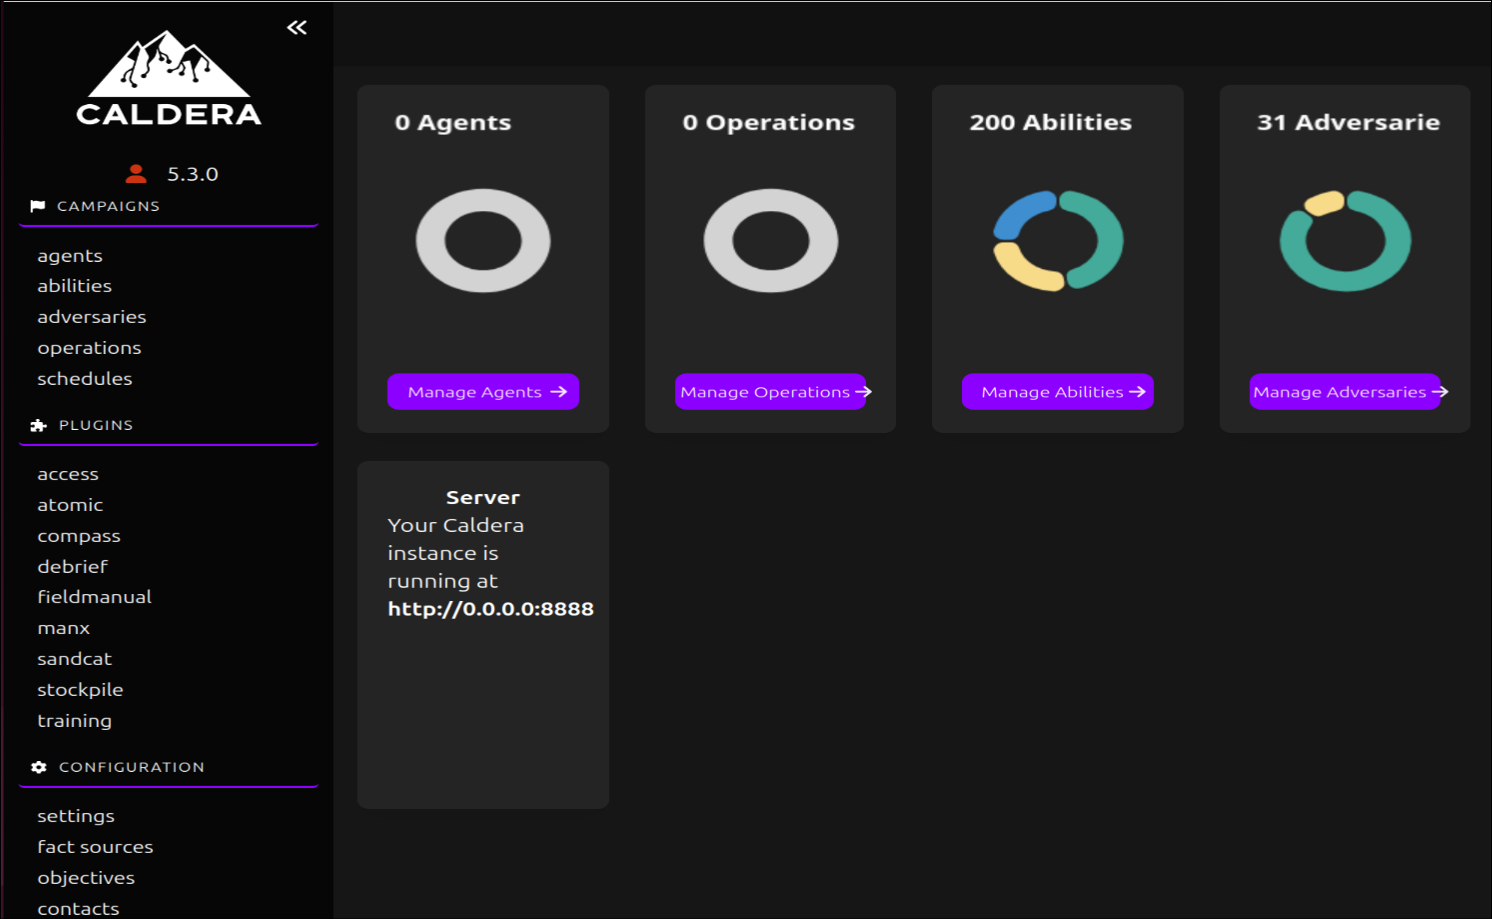
\includegraphics[width=1\linewidth]{figures/Caldera_dashboard_red.png}
    \caption{MITRE Caldera's Red Dashboard }
    \label{fig:Caldera_dashboard_red}
\end{figure}

\begin{figure}
    \centering
    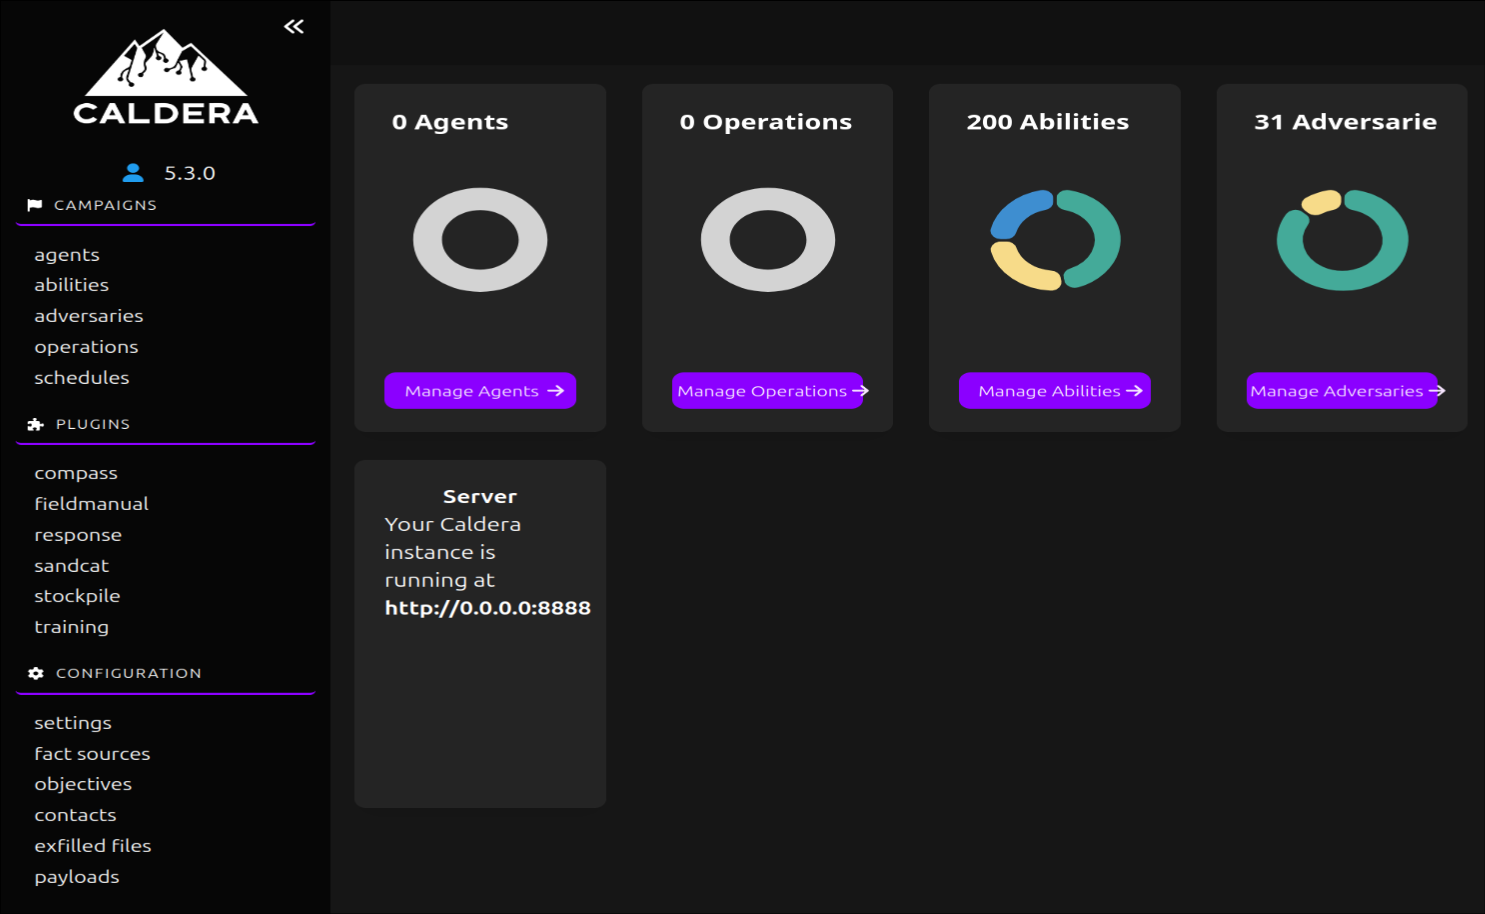
\includegraphics[width=\linewidth]{figures/Caldera_dashboard_blue.png}
    \caption{MITRE Caldera's Blue Dashboard}
    \label{fig:Caldera_dashboard_blue}
\end{figure}

\begin{itemize}
    \item \textbf{Knowledge and Operational Flow}\\
The platform's intelligence is driven by Facts, which are pieces of information (like IPs or usernames) about the network or host. These facts are collected by Parsers from the output of executed abilities and are crucial for the simulation's adaptive behavior, as they are used to substitute variables in subsequent commands, allowing the adversary to progress intelligently through an attack chain. The complete simulation is tracked through Operations, which record all actions. Caldera's functionality is sustained by clear technical prerequisites, requiring a Linux or macOS server with Python 3.8+ and NodeJS v16+, with GoLang 1.17+ recommended for dynamic agent compilation to aid in antivirus evasion. All server settings, C2 contacts, and API keys are managed through YAML configuration files.

\item \textbf{Core Capabilities and Plugins}\\
Caldera supports the full spectrum of cyber conflict through specialized capabilities and an extensive Plugin Architecture:
\begin{itemize}
    \item \textbf{Autonomous Red and Blue Engagements:} The framework facilitates fully Autonomous Red-Team Engagements to test defenses and Autonomous Incident-Response operations, where defensive profiles automatically execute counter-actions based on collected network facts.
    
    \item \textbf{Access and Movement:} The platform enables the simulation of initial intrusion stages, including Initial Access Attacks (Pre-ATT\&CK and Initial Access tactics) and Lateral Movement. Lateral movement, often seen in Windows environments, involves moving the agent binary to a new host and remotely executing it (via service creation or WMI) to establish a new C2 connection.
    
    \item \textbf{Exfiltration Methodology:} Data theft is a multi-step process governed by the Stockpile plugin. This involves first using the Advanced File Search and Stager ability to locate files and move them to a hidden staging directory. The staged files are then typically compressed, encrypted (often password-protected), and finally transferred to external destinations like Dropbox, GitHub, or AWS S3 that have been pre-configured in the Fact Source.
\end{itemize}

    \item \textbf{Key Plugin Functions:}
\begin{itemize}
    \item \textbf{Stockpile:} Serves as the core content repository for abilities and adversaries.
    \item \textbf{Sandcat:} Provides the flexible, modular agent that supports multiple C2 communication channels (HTTP(S), DNS Tunneling) and Peer-to-Peer Proxy capabilities via gocat extensions.
    \item \textbf{Response:} Offers content for autonomous defensive actions.
    \item \textbf{Debrief:} Provides campaign analytics, visualization, and detailed reporting.
    \item \textbf{Atomic:} Imports tests from the Red Canary Atomic repository for expanded emulation content.
\end{itemize}
\end{itemize}

Figure~\ref{fig:caldera_agents} shows the Agents management interface in Caldera, showing a deployed agent with a unique ID (paw), its host, assigned group (red), platform (linux), contact method (HTTP), and current status (alive, trusted). This interface allows operators to monitor and manage their implants across the network.

\begin{figure}
    \centering
    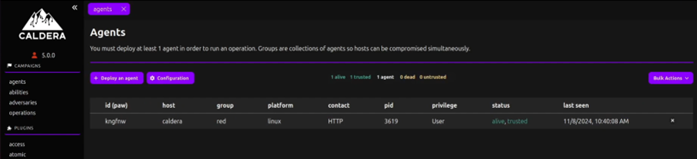
\includegraphics[width=1\linewidth]{figures/Figure22.png}
    \caption{MITRE Caldera’s Agents management}
    \label{fig:caldera_agents}
\end{figure}

The Abilities section, depicted in Figure~\ref{fig:caldera_abilities}, showcases the vast library of attack and defense techniques available within Caldera. Each entry represents a specific ATT\&CK tactic/technique, detailing its name (e.g., ``C2 Data Exfiltration'' or ``Compress Staged Directory''), the associated MITRE ATT\&CK ID (e.g., T1041 or T1560.001), and a brief description of its function. This interface allows users to search, filter by platform or plugin, and select the precise TTPs needed for their emulation scenarios.

\begin{figure}
    \centering
    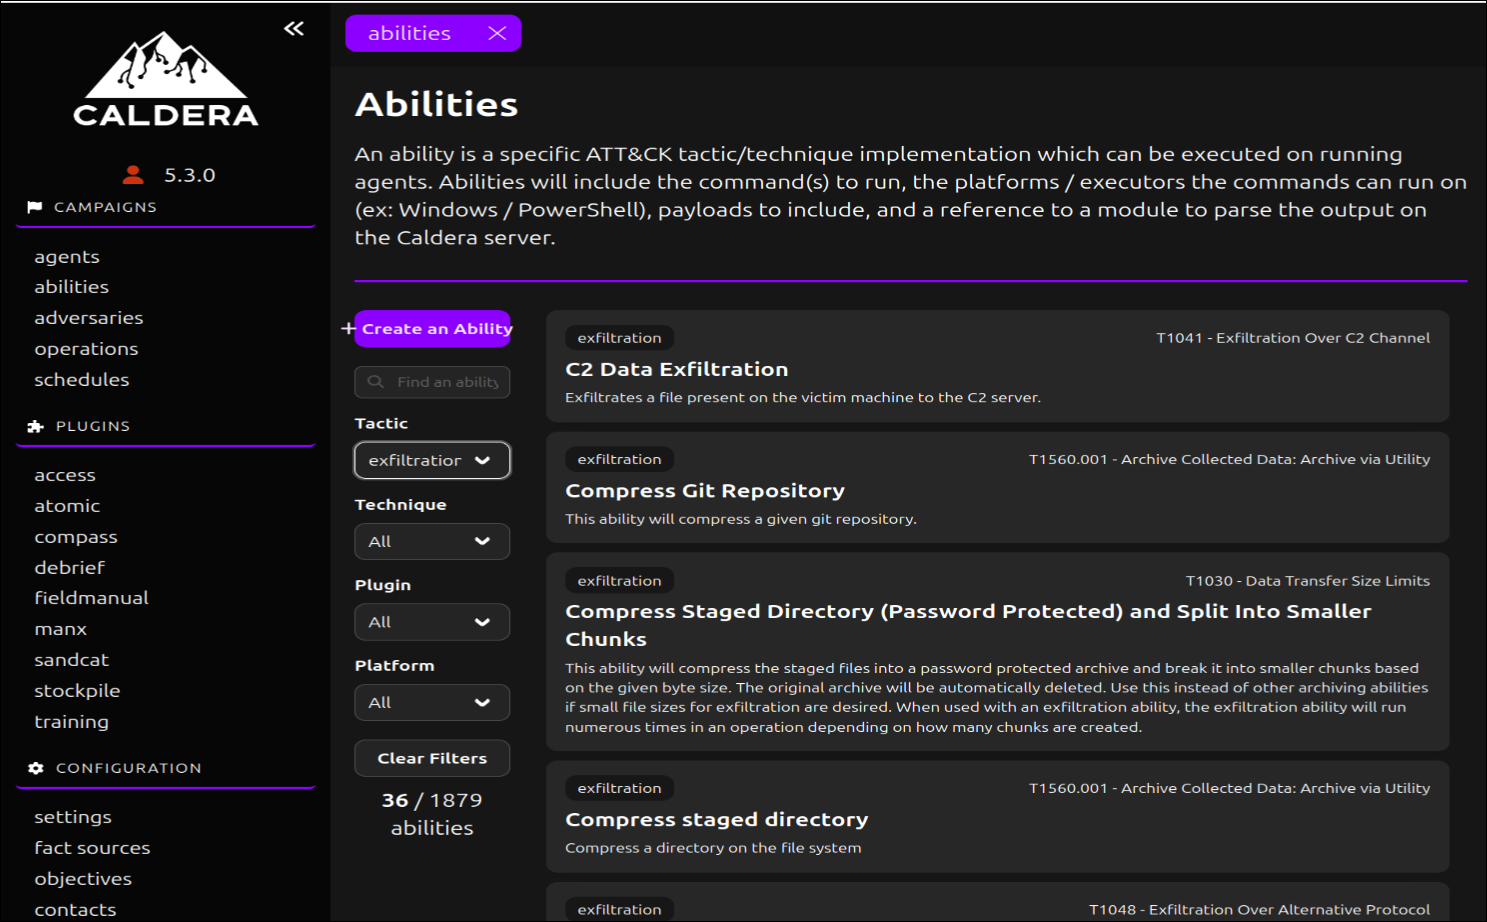
\includegraphics[width=1\linewidth]{figures/Caldera_Abilities.png}
    \caption{MITRE Caldera's Abilities interface}
    \label{fig:caldera_abilities}
\end{figure}

 \begin{itemize}
     \item \textbf{Analysis and Reporting}
 Upon completion of an operation, Caldera generates two essential, structured JSON reports for post-operation analysis, critical for forensic investigation and security monitoring evaluation:
    \begin{itemize}
    \item \textbf{Operation Report:} This is a comprehensive, nested summary that includes the full Adversary Profile, the selected Planner, the complete list of all Facts collected, and detailed, step-by-step execution records, along with their ATT\&CK mapping (Tactic and Technique ID). It is primarily used for deep forensic and research analysis.

    \item \textbf{Operation Event Logs:} This is a ``flattened'' list of execution events optimized for direct ingestion into SIEM tools. It focuses specifically on the successfully executed commands and includes agent/ability metadata, execution timestamps, and ATT\&CK mappings, allowing defenders to validate their security detection and logging capabilities against the simulated TTPs.
    \end{itemize}
\end{itemize}

%-----------------------------|    2.4 Infection Monkey    |------------------------------------|
\section{Infection Monkey}\label{sec:Infection}
Infection Monkey\cite{monkey_docs} is a comprehensive, open-source Breach and Attack Simulation (BAS) tool designed to continuously test an organization’s resilience against internal server infection and lateral movement. It safely simulates the behavior of a worm-like binary program, providing security teams with an empirical, attacker-centric view of their internal network to validate existing security controls and identify hidden security gaps.

\begin{figure}
    \centering
    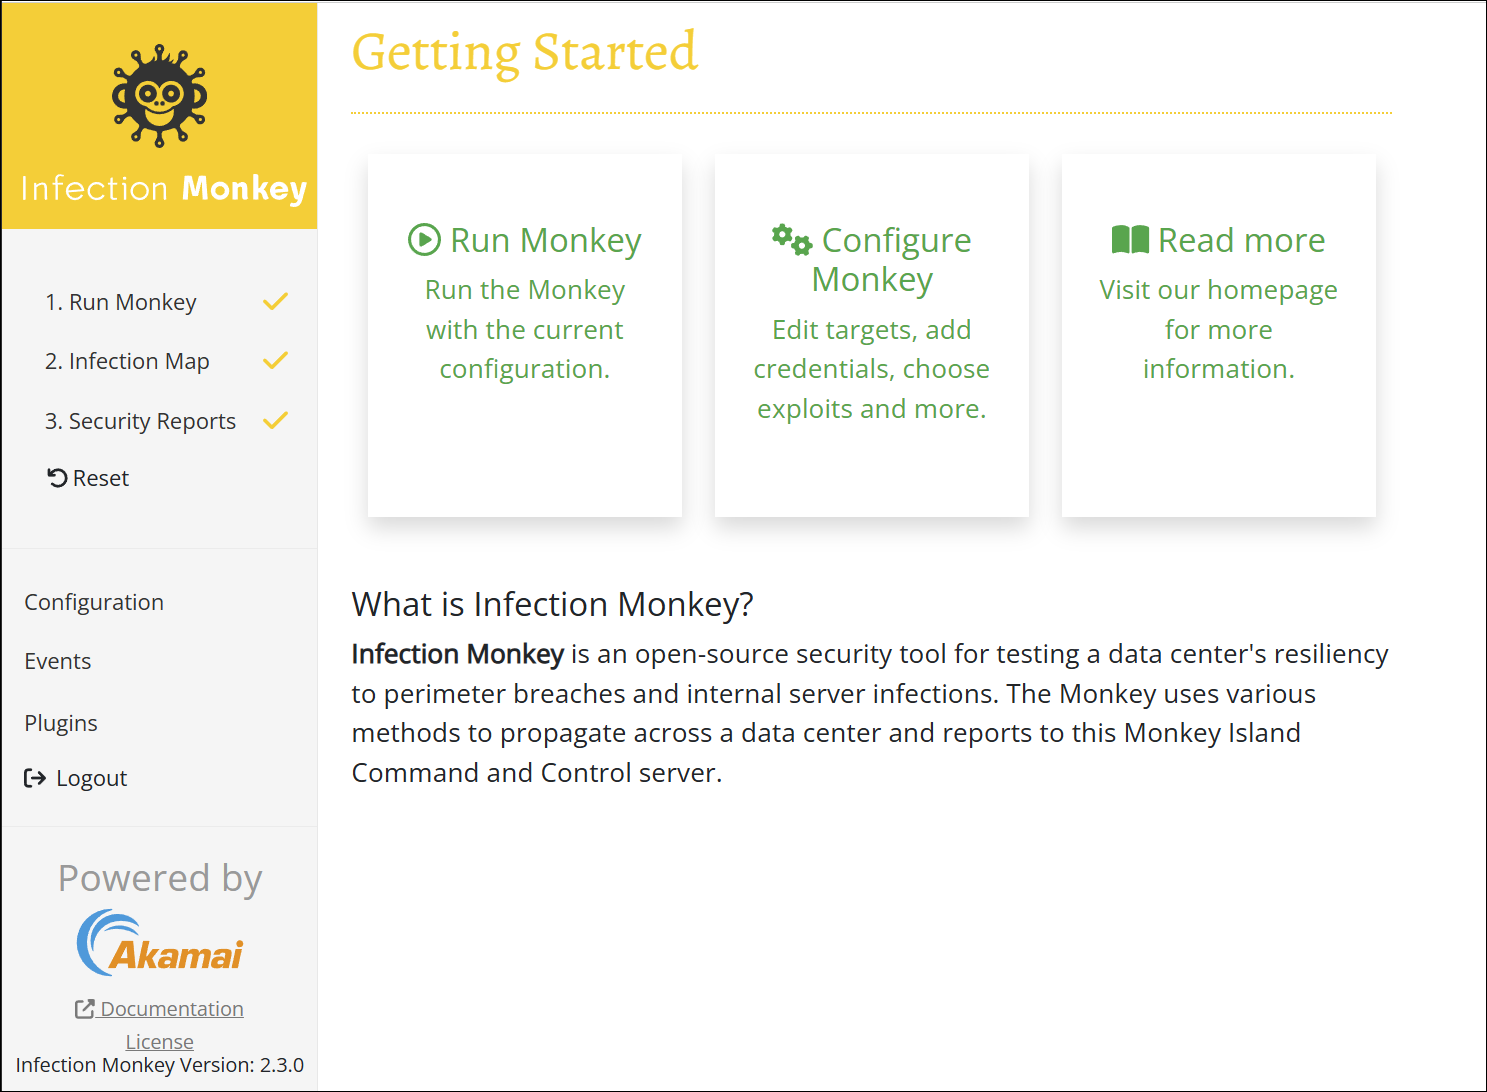
\includegraphics[width=1\linewidth]{figures/Getting Started.png}
    \caption{Infection Monkey's Island Dashboard }
    \label{fig:monkey_dashboard}
\end{figure}

Figure~\ref{fig:monkey_dashboard} displays the Monkey Island central dashboard. This interface provides direct access to essential workflows, allowing operators to configure attack parameters, launch simulations, and navigate to reporting modules via the sidebar.

\begin{itemize}
    \item \textbf{Core Architecture and Methodology}

The Infection Monkey platform is composed of two primary, communicating components:

\begin{itemize}
    \item \textbf{Monkey Agent (Monkey):} The core simulation tool. This is a safe, worm-like binary configured to autonomously scan the local network, attempt propagation to other machines using safe exploiters, and simulate various post-breach attack techniques without causing permanent damage.

    \item \textbf{Monkey Island Server (Island):} The centralized Command and Control (C\&C) web server. It handles the UI, manages the simulation configuration, aggregates all collected data, and presents the final reports and network visual maps.
\end{itemize}

The overall methodology centers on controlled network propagation. Agents spread based on pre-defined configuration parameters (which can include credentials, network segment rules, or specific attack scenarios), replicating an attacker's discovery and lateral movement techniques. The simulation uses only safe exploiters and is engineered to avoid permanent system modifications.
    \item \textbf{Simulation Capabilities and Scenarios}
Infection Monkey is highly versatile, offering core features and custom scenarios to fine-tune testing for specific defensive needs. The simulation workflow is enabled through an extensible plugin system and can be initiated either ``From Island'' (starting on the C\&C machine) or ``Manual'' (running the agent on a specific compromised host).
    \item \textbf{Key simulation capabilities and scenarios include:}
 \begin{itemize}
     \item \textbf{Ransomware Simulation:} Tests data manipulation defenses by simulating ransomware behavior. The agent encrypts files in a user-specified directory using a fully reversible bit-flip algorithm and replicates ransom note placement.
    \item \textbf{Network Breach:} Simulates lateral propagation starting from an already compromised internal host (e.g., a database server) to assess the blast radius of an initial breach.
    \item \textbf{Network Segmentation:}  Verifies the efficacy of isolation policies. Users define subnets that should be segregated, and the Monkey verifies isolation by attempting simple cross-segment ping tests. Isolation failures are detailed in the Security Report.
    \item \textbf{Credentials Leak:} Assesses the impact of stolen credentials. Users can input real credentials (usernames and passwords) or allow the Monkey to collect discovered SSH key pairs, which the agent then automatically reuses to facilitate lateral movement across the network.
 \end{itemize}

    \item \textbf{Platform and Deployment Support}

The platform is designed for broad accessibility, with all components running on x86-64 processors.

    \begin{itemize}
        \item The \textbf{Monkey Agent} offers a minimal footprint and supports a wide range of operating systems, including Linux (GLIBC $\ge$ 2.23) and Windows (Windows $\ge$ 2012).
    
        \item The \textbf{Monkey Island Server}, which serves as the central command and control, runs natively on modern Linux distributions (via AppImage) and Windows Server 2016/2019/Windows 10. Note that the server component requires significant resources, specifically a minimum of 4 CPU Cores and 6GB RAM for Windows Server environments.

        \item Deployment methods are flexible, including Windows Installer, Linux AppImage, Docker (Linux-only), and a dedicated AWS Marketplace AMI. The AMI deployment specifically requires inbound TCP traffic on port 5000.
\end{itemize}

Figure~\ref{fig:monkey_map} presents the Infection Map, which visualizes the attack topology. It depicts the central ``Monkey'' agent initiating network scans against discovered Windows targets, with orange directional lines indicating the flow of reconnaissance.

\begin{figure}
    \centering
    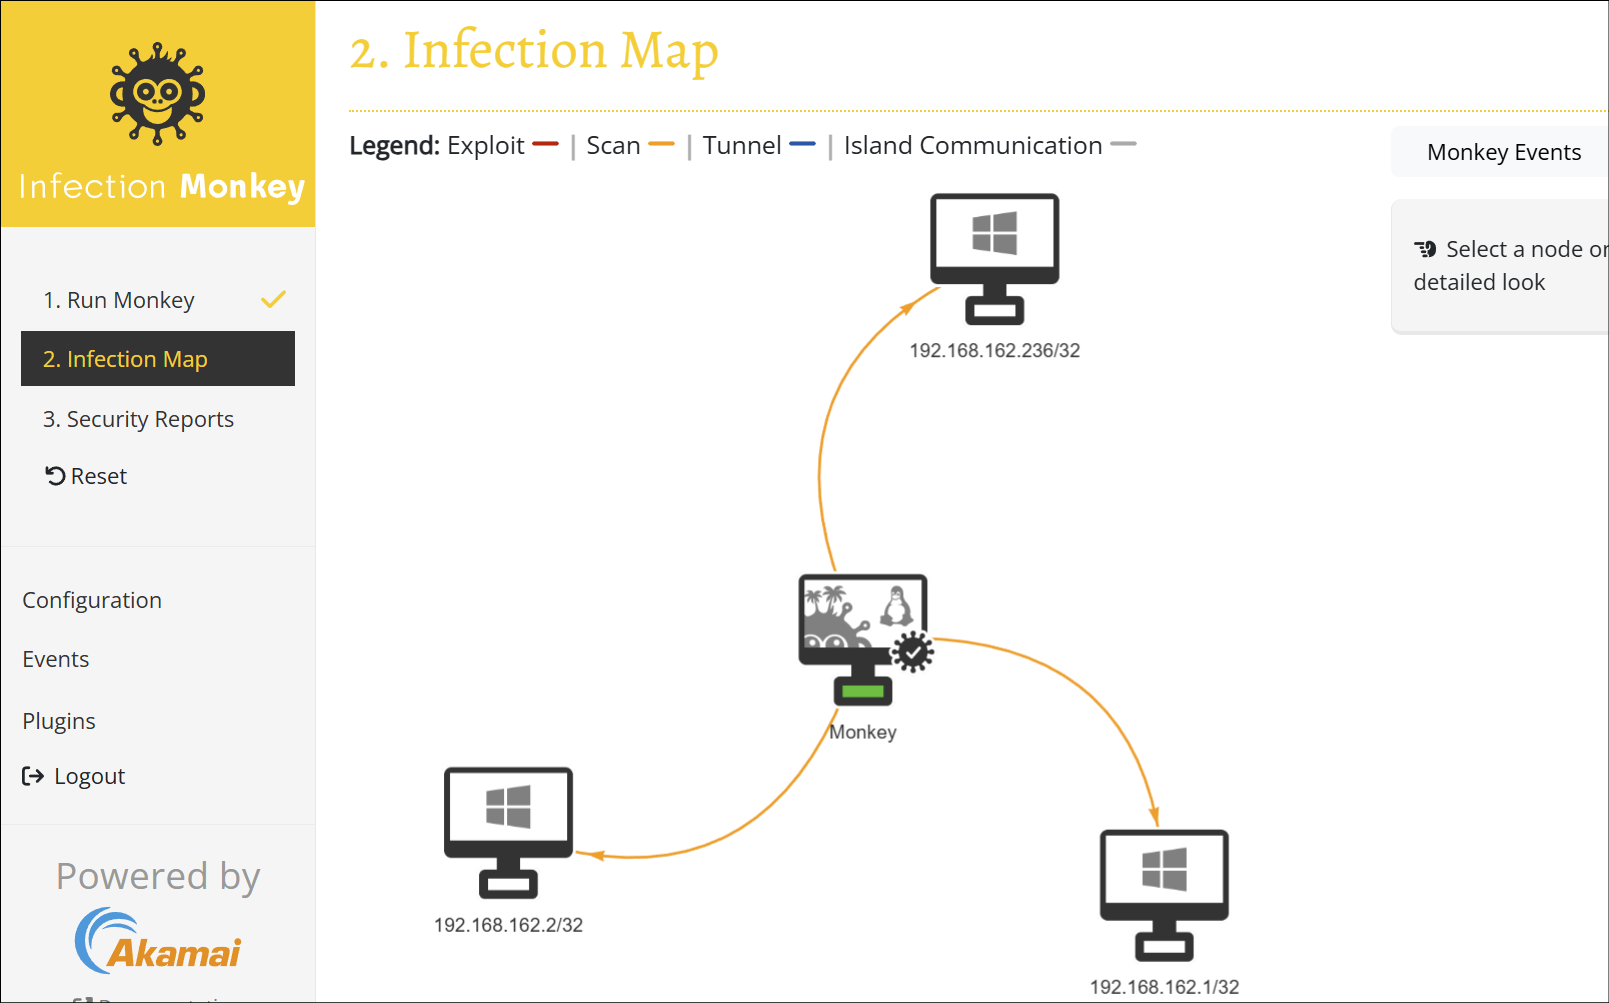
\includegraphics[width=1\linewidth]{figures/Infection Map.png}
    \caption{Infection Monkey's Network Propagation Map}
    \label{fig:monkey_map}
\end{figure}

    \item \textbf{Analysis and Reporting}

The results of the simulation are translated into actionable security improvements via detailed reports, primarily the Security Report. This comprehensive report provides mitigation steps and is organized into sections that detail:

         \begin{itemize}
             \item \textbf{Security Report:} The comprehensive primary report provides actionable mitigation steps and is split into sections that detail:
       
            \begin{enumerate}
                 \item High-Level Execution
                 \item Segmentation Issues
                 \item Machine-related Recommendations
                 \item The Network from the Monkey's Eyes (a summary of scanned, breached, and credential theft activities)
            \end{enumerate}

            \item \textbf{Ransomware Report}: A dedicated report that details the successful ransomware simulation in three sections:
            \begin{enumerate}
                 \item Breach (entry point)
                 \item Lateral Movement (propagation path)
                 \item Attack (list of specific files successfully encrypted)
            \end{enumerate}
        \end{itemize}
      \end{itemize}

\begin{figure}
    \centering
    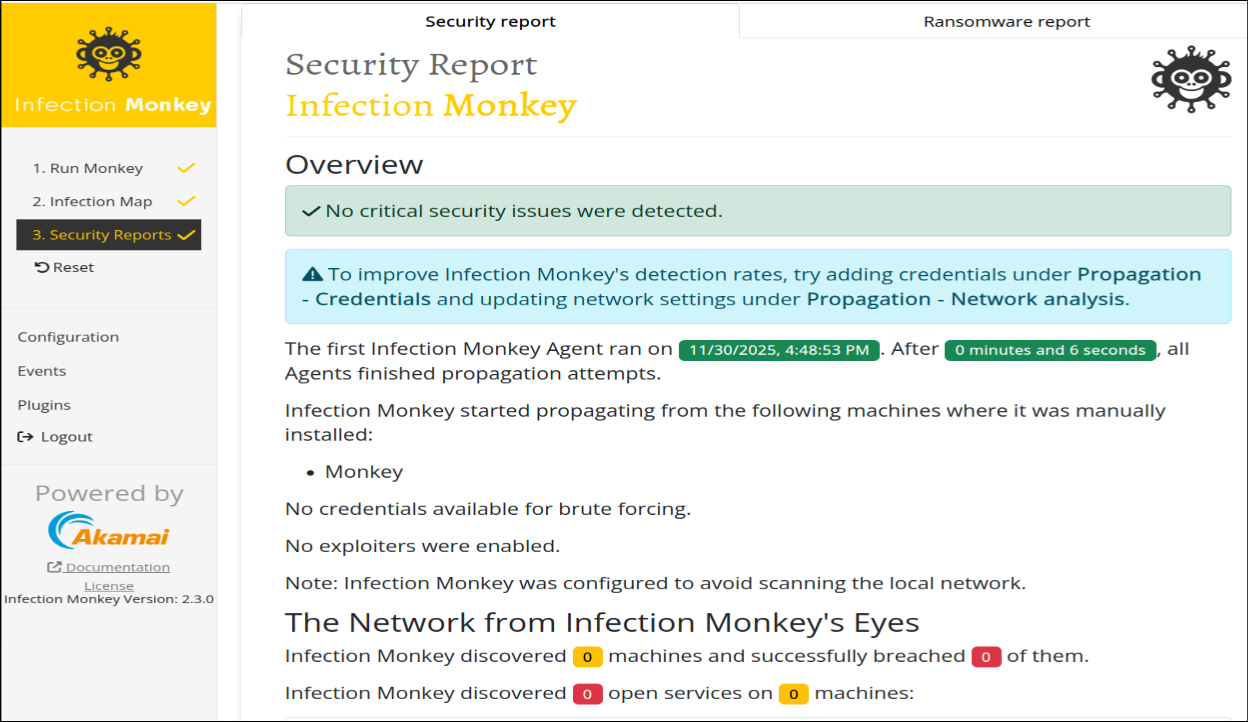
\includegraphics[width=1\linewidth]{figures/SecurityReport.png}
    \caption{Infection Monkey's Security Report}
    \label{fig:monkey_reports}
\end{figure}

Figure~\ref{fig:monkey_reports} shows an example of the Security Report in the Monkey Island UI. The overview highlights a critical security issue detected and details the attack's initiation, including the machine from which propagation started (island-linux-250), the usernames available for brute-forcing (e.g., Administrator, m0nk3y), and the sensitive credentials available for brute-forcing (e.g., LM hash, NT hash, Clear SSH private key, Clear Password). This section immediately demonstrates the quality of information an attacker could leverage and the starting point of the lateral movement within the network.

\begin{figure}[htbp]
    \centering
    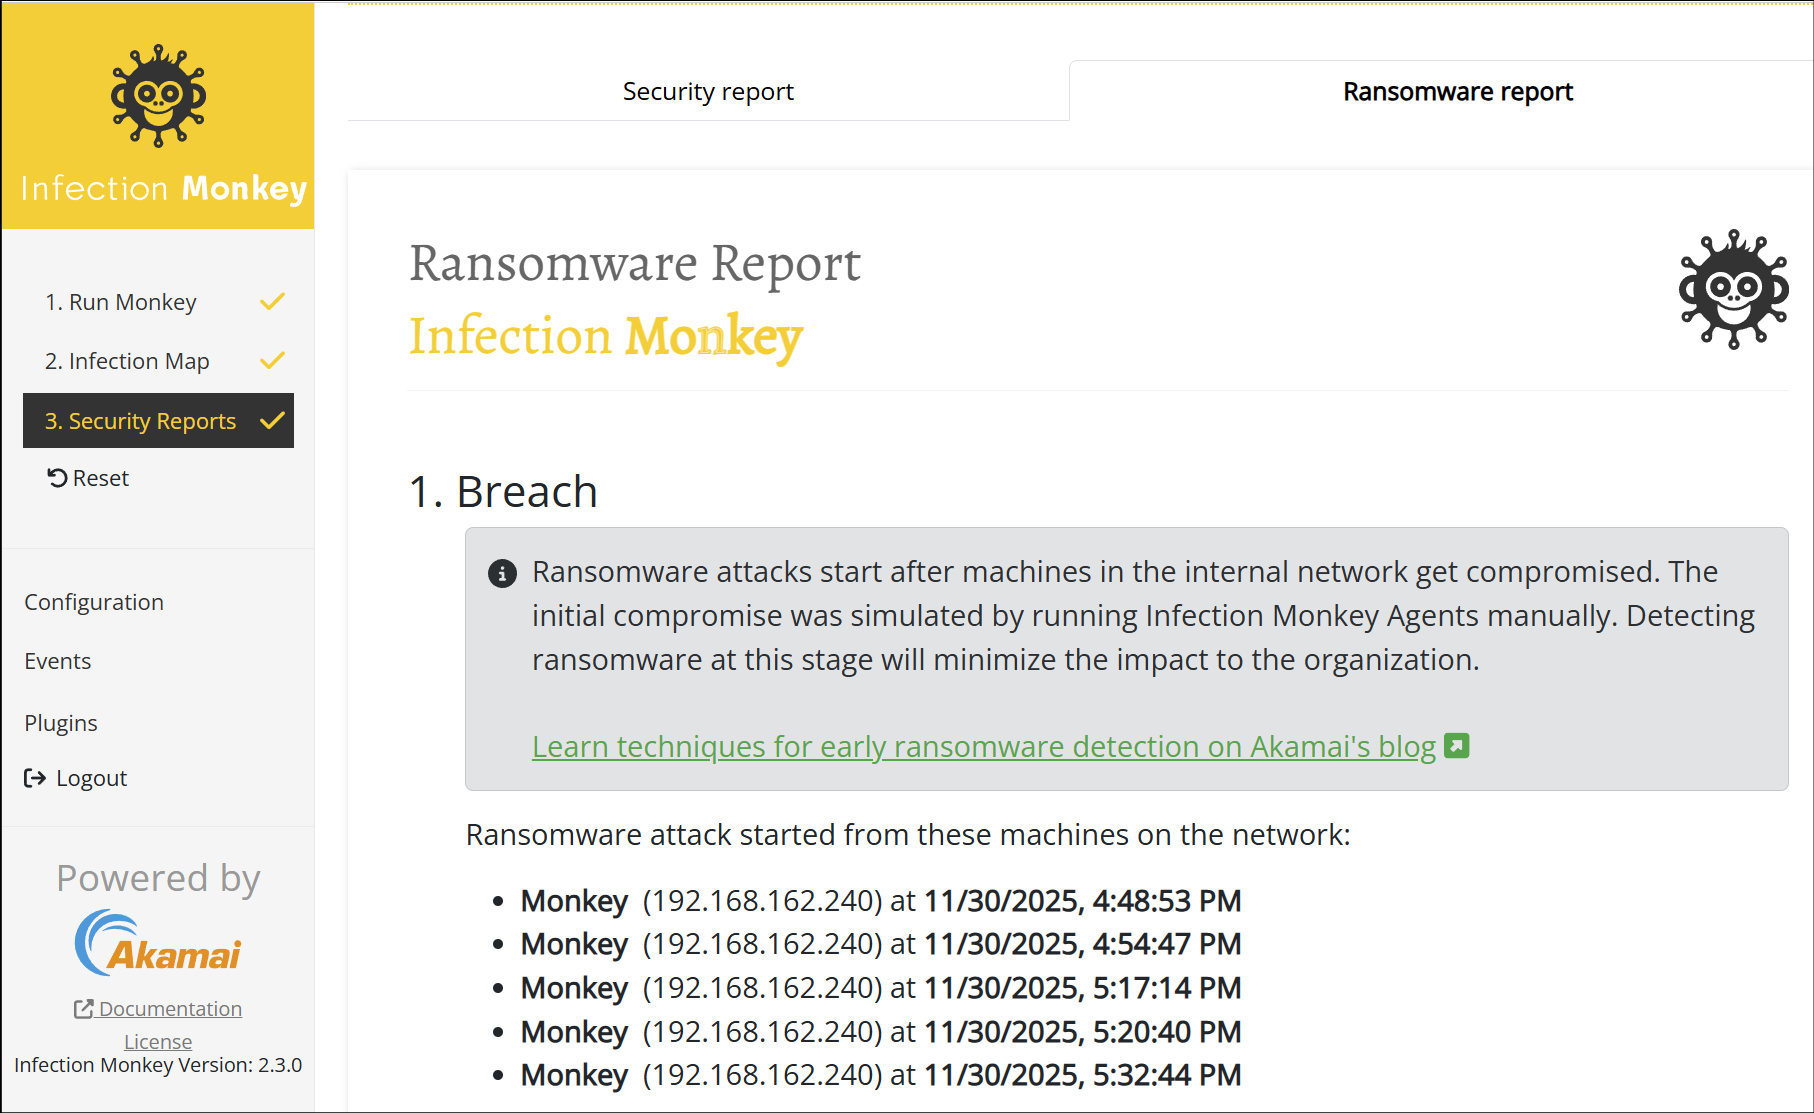
\includegraphics[width=1\linewidth]{figures/RansomwareReport.png}
    \caption{Infection Monkey's Ransomware Report}
    \label{fig:monkey_ransomware_report}
\end{figure}

Figure~\ref{fig:monkey_ransomware_report} displays the Ransomware Report interface. It details the initial ``Breach'' phase, logging the source machine (192.168.162.240) and specific execution timestamps. The report follows the attack chain, explicitly separating the initial entry point from subsequent lateral movement attempts.

%---------------------------|    2.5 Atomic Red Team   |---------------------------------------|
\section{Atomic Red Team}\label{sec:Atomic}
The Atomic Red Team\cite{atomic_docs} is a free and open-source library of scripted cyberattacks that serves as a fundamental resource for security teams seeking to systematically assess and validate their security controls. It functions as a community-driven, accessible alternative to proprietary Breach and Attack Simulation software. The project's primary objective is to operationalize adversary tradecraft by providing detailed procedures for defense validation.

\begin{figure}
    \centering
    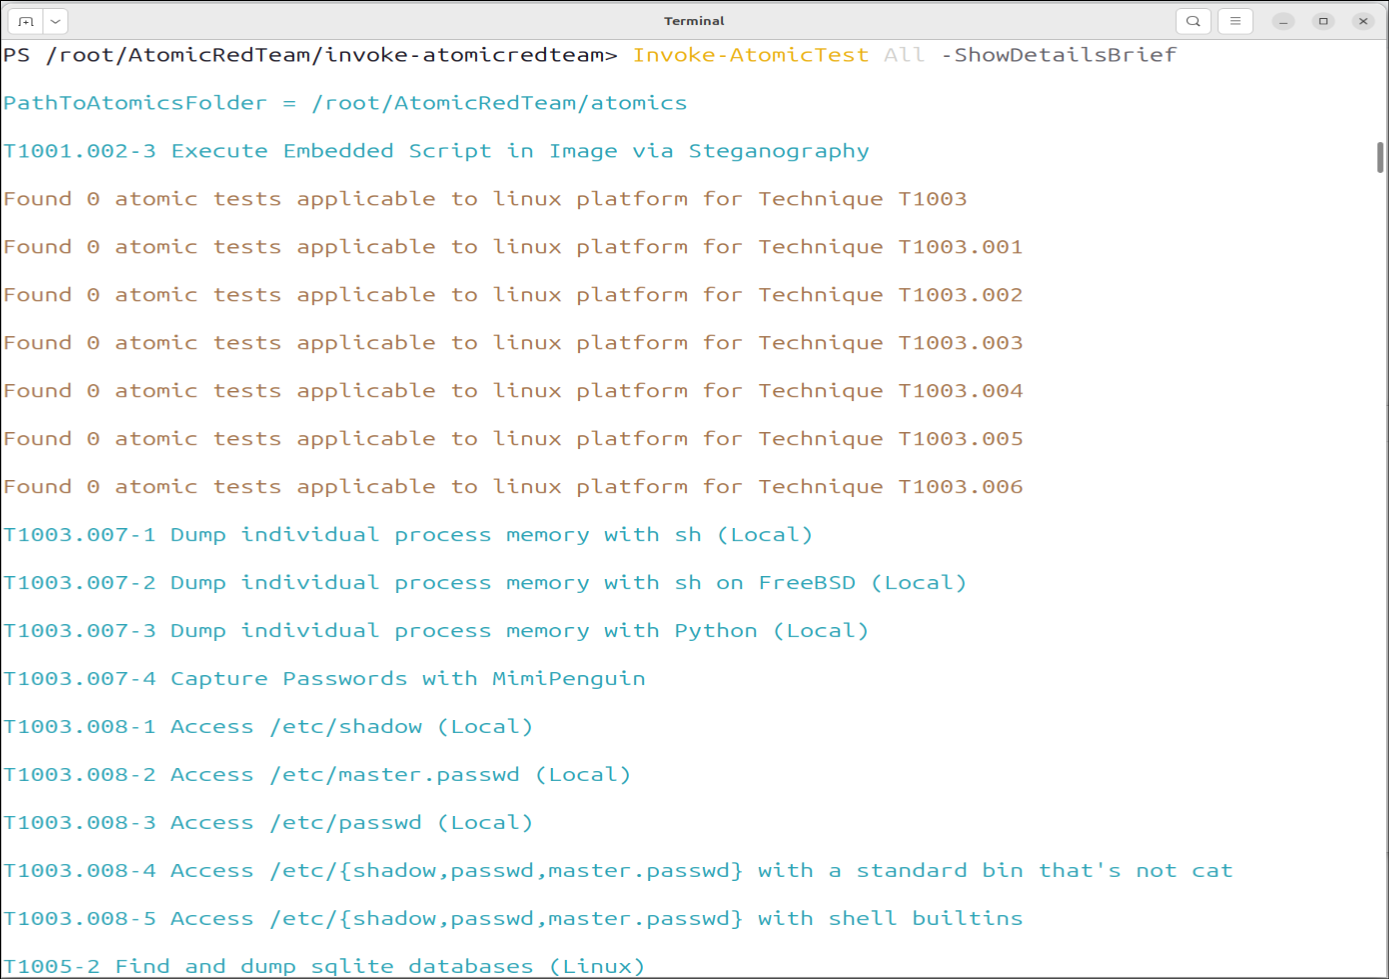
\includegraphics[width=1\linewidth]{figures/Canary_framework.png}
    \caption{Atomic Red Team's MITRE ATT\&CK lists}
    \label{fig:Canary_mitreid}
\end{figure}

Figure~\ref{fig:Canary_mitreid} displays the output of the \textit{Invoke-AtomicRedTeam} command. The framework filters and lists atomic tests applicable to the Linux platform, categorized by MITRE ATT\&CK technique IDs.

\begin{itemize}
    \item \textbf{Foundational Methodology}

The core methodology of the Atomic Red Team is its strict alignment with the MITRE ATT\&CK® matrix. The library fills a gap in the MITRE framework by translating abstract techniques into concrete, executable procedures, known as Atomic Tests.

    \item \textbf{Key characteristics of the tests include:}
        \begin{itemize}
            \item \textbf{Efficiency:} Designed to run quickly, often in five minutes or less.
             \item \textbf{Structure:} Each test is indexed by its MITRE ATT\&CK ID (T-number) and includes prerequisites, attack commands, optional cleanup commands, and input arguments for customization.
        \end{itemize}
    \item \textbf{Operational Frameworks and Tools}

The Atomic Red Team ecosystem provides several specialized, cross-platform tools to execute and validate the library's procedures.

\begin{itemize}
    \item \textbf{Invoke-AtomicRedTeam (Execution)}
    
Invoke-Atomic is the dedicated PowerShell execution framework used to manage and run the atomic tests, simplifying complex execution workflows.


\begin{itemize}
    \item \textbf{Capabilities:} It supports cross-platform execution (Windows, macOS, Linux) via PowerShell Core, enables remote execution through PowerShell remoting, and automates critical steps like checking and installing prerequisites (Get Prereq Commands), substituting input arguments, and running cleanup commands.

    \item \textbf{Atomic Runner:} A component of the framework designed for enterprise use, facilitating the orchestration of scheduled tests across multiple machines and ensuring proper logging via unique GUIDs and host names for detection correlation.
\end{itemize}

\item \textbf{Specialized Validation Tools}
        \begin{itemize}
            \item \textbf{AtomicTestHarnesses:} A library (utilizing PowerShell and Python) crucial for validating the telemetry generated during execution. It is designed to stress test detection systems by running many variations of a single technique to evaluate the depth and fragility of security coverage.
            \item \textbf{Chain Reactor:} An open-source framework dedicated to composing executables that simulate adversary behaviors specifically on Linux endpoints. It uses easily configurable JSON input files.
        \end{itemize}
    \end{itemize}
    \item \textbf{Test Design and Contribution Standards}

The community-driven nature of Atomic Red Team necessitates strict guidelines for test development to ensure consistency and utility.

\begin{itemize}
    \item \textbf{Cleanup and Dependencies:} Cleanup commands must be designed to be repeatable without generating errors. External dependencies should not be committed directly but must be downloaded from their original sources using the prereq commands YAML key, often via permanent GitHub links.

    \item \textbf{Portability:} New tests must be as portable as possible, relying on environment variables instead of hard-coded paths, and favoring \texttt{sh} over \texttt{bash} for Linux.

    \item \textbf{Documentation:} Tests must be accompanied by clear descriptions, the expected output, and links to external resources that detail the attack.
\end{itemize}

    \item \textbf{Best Practices and Security Responsibility}

The framework's core value is its capacity to move an organization past security based on ``hope''.

\begin{itemize}
    \item \textbf{Testing Philosophy:} Best practice dictates testing should occur in two phases: first, with blocking controls OFF to ensure comprehensive detection telemetry is collected, and second, with blocking controls ON to evaluate prevention efficacy. The guiding principle cited is: ``Prevention is ideal, but detection is a must''.

    \item \textbf{Safety and Responsibility:} Users must always obtain permission before testing and execute all procedures in a dedicated non-production or lab environment, as tests may leave the system in an undesirable state.
    \end{itemize}
\end{itemize}
\begin{figure}[htbp]
    \centering
    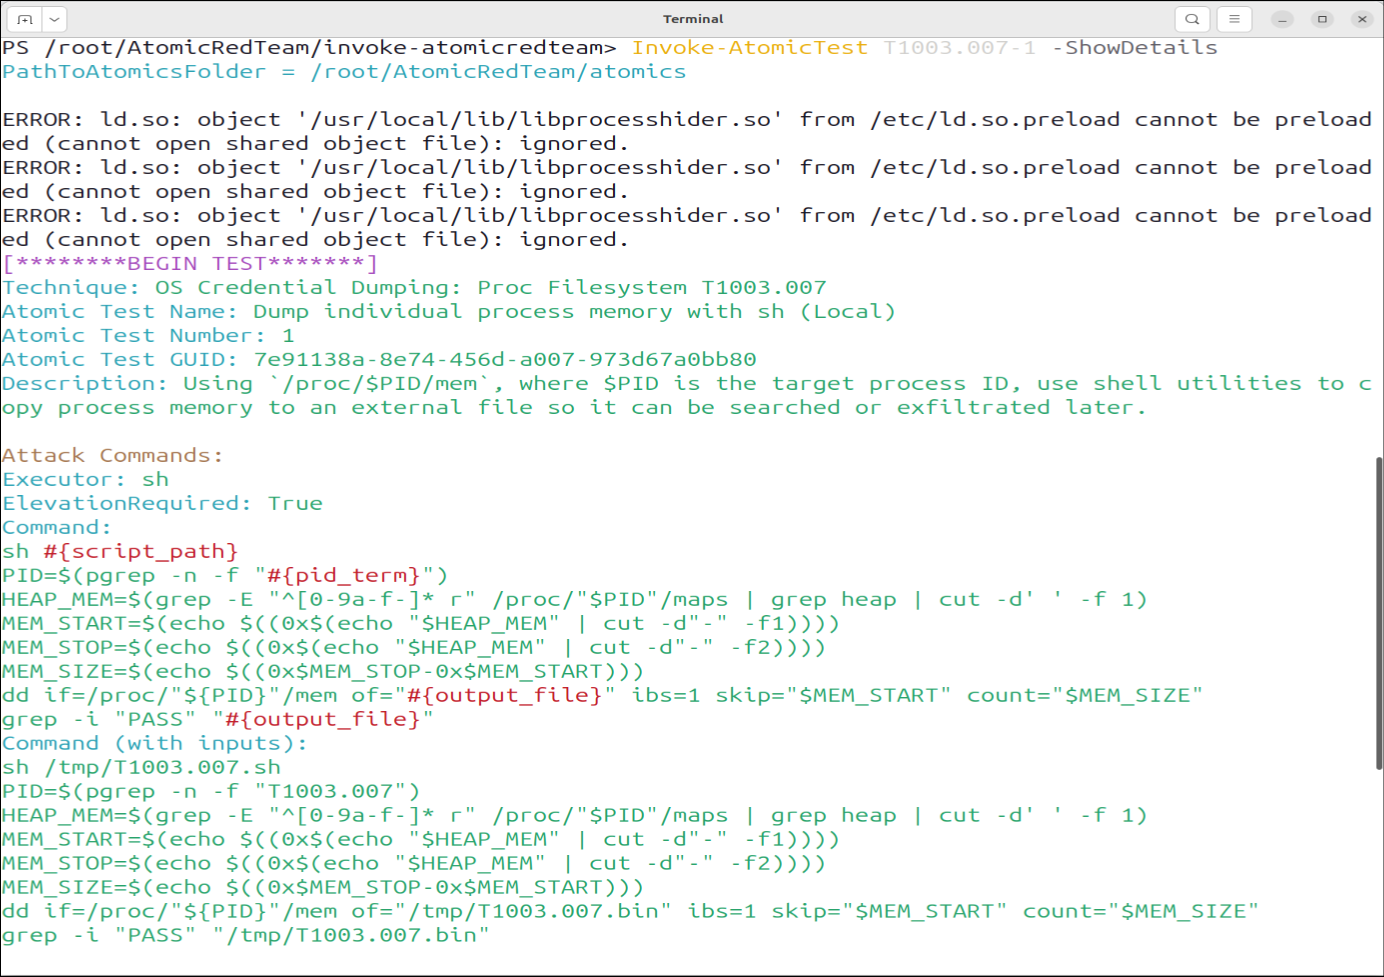
\includegraphics[width=1\linewidth]{figures/Canary_EX-Attack.png}
    \caption{Atomic Red Team's execution logic example}
    \label{fig:example_attack}
\end{figure}

Figure~\ref{fig:example_attack} shows an example of the detailed configuration for Atomic Test T1003.007-1, which simulates OS Credential Dumping via the Proc Filesystem. The output reveals the specific shell commands utilized to perform the attack, demonstrating how the \texttt{dd} utility is used to extract the heap memory of a target process from \texttt{/proc/\$PID/mem} for credential analysis.

%---------------------------|    2.6 Related Work   |--------------------------------------|
\section{Related Work}
The shift from manual penetration testing to automated security validation is a major trend in cybersecurity. However, few studies directly compare open-source Breach and Attack Simulation (BAS) tools. Most existing research focuses either on qualitative feature comparisons or theoretical models. 

\subsection{Red Team Redemption: A Structured Comparison of Open-Source Tools for Adversary Emulation}
Landauer et al.\cite{landauer2024} provide a foundational baseline in their work, "Red Team Redemption," which conducted a comprehensive survey and ranking of 9 adversary emulation tools: ATTPwn, Atomic Red Team, APTSimulator, MITRE Caldera, DumpsterFire, Infection Monkey, Invoke Adversary, Metaspoit and Purplesharp. Their study utilized a mixed-method approach comprising three interconnected components that all relied on a single master list of features:
\begin{itemize}
    \item \textbf{Questionnaire Assessment:} The establishment of a theoretical framework evaluating 80 specific criteria across 5 core categories: Installation \& Configuration, Community \& Support, Documentation, Usability, and Features \& Capabilities.
    \item \textbf{Offline Tool Assessment:} A hands-on technical evaluation to verify basic functional requirements, utilizing offline checklists that directly mapped to the 80 criteria established in the questionnaire phase.
    \item \textbf{User Requirement Survey:} A survey asking cybersecurity domain experts to assign importance weights to these exact same 80 criteria in order to calculate an overall tool ranking.
\end{itemize}

While Landauer’s 80-question framework provides a foundational taxonomy, this study operationalizes these criteria through a high-fidelity laboratory environment. By narrowing the scope to Installation \& Configuration and Features \& Capabilities, the research transitions from qualitative assessment to direct technical verification. This approach focuses exclusively on reproducible telemetry—such as exact deployment sequences, resource overhead, and execution stability—while intentionally excluding subjective, survey-based categories like Documentation and Usability. This ensures the evaluation is grounded in the empirical reality of tool deployment rather than aesthetic or manual-based preferences.

\subsection{A Unified Modeling Framework for Automated Penetration Testing}
Wang et al. \cite{wang2025} address the theoretical fragmentation in automated penetration testing (AutoPT) by proposing a standardized modeling framework. Analyzing and categorizing 65 studies, they introduced the Multi-Dimensional Classification System (MDCPM) and a practical simulation engine to support AI agent training. Their work comprises three core components:
\begin{itemize}
    \item \textbf{MDCPM Classification:} A theoretical system categorizing literature into four dimensions: Literature Objectives, Network Complexity, Dependency of Technical and Tactical Operations, and Scenario Feedback.
    \item \textbf{AutoPT-Sim Framework:} A unified modeling framework designed to simulate dynamic network environments, attackers, and defenders.
    \item \textbf{Public Dataset and Generator:} The release of a standard network environment dataset and a "Network Generator" tool for fair algorithm comparison.
\end{itemize}

While Wang et al. provide a robust theoretical foundation, their framework relies on abstract models rather than empirical software execution. This research bridges that gap by operationalizing their MDCPM classification within a controlled laboratory environment. Specifically, their requirement for dynamic scenario feedback is translated into our Threat Intelligence Alignment evaluation, while the need for coordinated technical operations is verified through Framework Extensibility testing. Furthermore, while Wang theoretically validates MITRE Caldera, they identify a scarcity of dynamically updated scenarios; we address this by empirically benchmarking tool update mechanisms and repository health. This transitions Wang’s theoretical concepts into reproducible laboratory parameters derived from the actual installation and execution of each BAS tool. 

\subsection{Cyber Attack Modeling and Simulation for Network Security Analysis}
Addressing the limitations of physical testbeds, Kuhl et al. \cite{kuhl2007} developed a discrete-event simulation framework to model computer networks and generate synthetic security data. Their work focused on creating a flexible environment for testing situational awareness tools through three core mechanisms:
\begin{itemize}
    \item \textbf{Network Abstraction:} They modeled infrastructure using logical constructs to represent network topology efficiently, specifically designed to avoid the computational overhead of packet-level simulation.
    \item \textbf{Multi-Stage Attack Generation:} Leveraging a graph-based guidance template, they implemented an attack model spanning ten distinct stages (from Reconnaissance to Goal/Pilfering), pre-dating but mirroring the structure of the MITRE ATT\&CK framework.
    \item \textbf{Synthetic Data Production:} The simulation generated comprehensive output datasets, providing "ground truth" logs of attacker actions mixed with background noise for defensive validation.
\end{itemize}

While Kuhl et al. prioritized scalability through abstraction, their approach inherently masks the physical impact of attack emulation on host systems. This study builds upon Kuhl’s concepts but shifts from a simulated environment to a high-fidelity physical laboratory. Specifically, where Kuhl sought to avoid 'computational overhead' through modeling, we treat system resource overhead as a primary performance indicator to quantify the actual hardware costs of BAS deployment. Furthermore, Kuhl’s 10-stage attack model underscores the necessity of evaluating Scenario Coverage for threat relevance in a live environment. Finally, whereas Kuhl produced 'synthetic ground truth logs,' this research evaluates the empirical execution reliability of actual malware payloads, ensuring that multi-stage attacks can execute without destabilizing the host during real-world installation.

\subsection{Implementation of Security Controls for the Treatment of Malware using Breach and Attack Simulation}

Focusing on the mitigation of ransomware and zero-day threats, Roque et al. \cite{roque2024} proposed a security architecture that integrates Breach and Attack Simulation (BAS) technology with the National Institute of Standards and Technology (NIST) framework. Their research aimed to optimize security controls through a continuous validation process:
\begin{itemize}
    \item \textbf{Architectural Design:} They implemented a layered defense strategy mapped to the NIST phases, utilizing Snort for IPS/IDS rules and Microsoft Defender for EDR.
    \item \textbf{Simulated Attack Execution:} Using the Picus Security platform as the BAS tool, they conducted randomized simulations of specific threats, such as the BlackByte Ransomware campaign.
    \item \textbf{Iterative Optimization:} Based on simulation findings, they refined security policies to address identified gaps, increasing their threat detection rate from an initial 47\% to 95\%.
\end{itemize}

While Roque et al. demonstrate that a BAS platform's value lies in its actionable output, their methodology is tethered to a premium commercial ecosystem. Their reported 95\% detection rate was achieved through high-fidelity remediation data from Picus to calibrate Snort and EDR signatures—a luxury often absent in non-commercial environments. This study addresses the resulting accessibility gap by investigating whether open-source alternatives can achieve operational parity. We operationalize Roque’s findings into our Quality of Reports evaluation, moving beyond simple binary logs to measure the presence of remediation intelligence, such as pre-configured signatures or automated fix scripts. By executing these tools in a physical laboratory, this research empirically tests if open-source frameworks can provide the remediation depth necessary to meet professional operational standards.


\subsection{The Research Gap}

Despite these foundational contributions, there is a critical lack of empirical evaluation of open-source BAS tools in real operational environments. While previous studies established theoretical needs or utilized commercial platforms, the following gaps remain, directly informing the Comparison Matrix of this study:
\begin{itemize}
    \item \textbf{Lack of Reliability Testing:} Studies like Landauer et al. \cite{landauer2024} used qualitative "functional checklists" to verify if features existed. They did not perform stress testing to measure actual execution reliability (i.e., whether the tools crash or fail when executed repeatedly in a live environment), which this study addresses through accurate Execution Reliability scoring.
    \item \textbf{No Resource Usage Data:} Theoretical frameworks (Wang et al. \cite{wang2025}), simulation models (Kuhl et al. \cite{kuhl2007}), and practical implementations (Roque et al. \cite{roque2024}) entirely omit system overhead measurements. Consequently, there is no existing empirical data on the actual computational cost (CPU and memory usage) of running these BAS servers. This study introduces a novel Operational Performance evaluation  to measure this critical factor for resource-constrained enterprises.
    \item \textbf{Actionable Output vs. Open-Source Reality:} While Roque et al. \cite{roque2024} validated that actionable reporting is mandatory for improving defenses, they relied on a premium commercial tool (Picus). There is currently no systematic comparison of whether free, open-source alternatives can generate the same caliber of actionable remediation data. This study directly tests this capability through the Quality of Reports assessment.
\end{itemize}

\begin{table}
    \caption{Literature Review Gap Analysis}
    \label{tab:gap_analysis}
    \centering
    \renewcommand{\arraystretch}{1.8} % Increases row height for better breathing room
    \begin{tabular}{>{\raggedright\arraybackslash}m{0.25\linewidth} >{\raggedright\arraybackslash}m{0.30\linewidth} >{\raggedright\arraybackslash}m{0.38\linewidth}}
        \toprule
        \textbf{Research} & \textbf{Limitation (The Gap)} & \textbf{How This Study Addresses It} \\ 
        \midrule
        
        Landauer et al. [16] & 
        Qualitative only; lacks real performance stress-testing. & 
        Replaces surveys with \textbf{empirical telemetry} for reliability and deployment. \\ \cmidrule(lr){1-3}
        
        Wang et al. [17] & 
        Purely theoretical; relied on abstract models. & 
        \textbf{Operationalizes} requirements into measurable laboratory tests. \\ \cmidrule(lr){1-3}
        
        Kuhl et al. [18] & 
        Used synthetic logs and abstracted overhead. & 
        Captures \textbf{physical laboratory measurements} of system overhead. \\ \cmidrule(lr){1-3}
        
        Roque et al. [19] & 
        Limited exclusively to a single premium platform (Picus). & 
        Evaluates \textbf{functional equivalence} in open-source remediation data. \\ 
        \bottomrule
    \end{tabular}
\end{table}

Table~\ref{tab:gap_analysis} summarizes the specific limitations of these foundational studies and illustrates exactly how this research addresses those outstanding gaps through targeted empirical metrics.

This study directly addresses these deficiencies by transitioning from abstract simulations and proprietary ecosystems to a reproducible, high-fidelity laboratory environment. By executing open-source BAS tools on physical hardware, this research generates original empirical telemetry regarding operational performance, execution stability, and deployment complexity—data points currently absent from the existing body of knowledge. % Literature Review
%==============================================================================%
%==========================|     CHAPTER 3 Method    |=========================%
%==============================================================================%
\chapter{Proposed Method} \label{chap:Method}
This chapter outlines the systematic approach used to evaluate the selected open-source Breach and Attack Simulation (BAS) tools. It focuses on creating a repeatable, evidence-based assessment of each tool’s usability and effectiveness. The methodology unfolds in four phases: establishing the conceptual framework, justifying the selection of MITRE Caldera, Infection Monkey, and Atomic Red Team, mapping their features in a comparison matrix, and finally, applying a scoring system to grade critical metrics like installation complexity and reporting quality.

%--------------------|    3.1 Conceptual Framework    |--------------------------------|
\section{Conceptual Framework}\label{sec:conceptual_framework}
To ensure a fair, systematic, and methodologically sound assessment of open-source Breach and Attack Simulation (BAS) tools, this study is governed by a structured conceptual framework (showed in Figure~\ref{fig:research_workflow}). This framework is specifically designed to isolate key variables, maintain consistent environmental factors, and guarantee the production of reliable and repeatable results across all tool deployments and test executions.

\begin{figure}
    \centering
    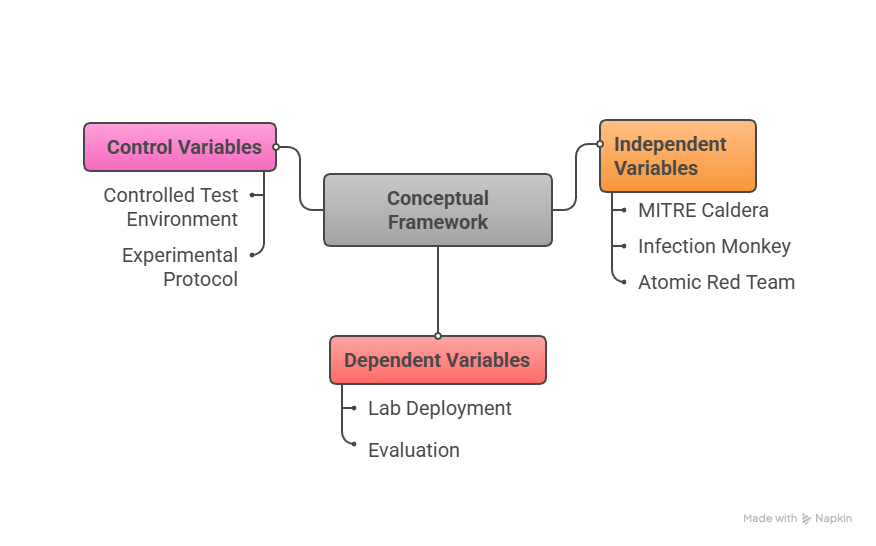
\includegraphics[width=1\textwidth]{figures/Conceptual Framework.png}
    \caption{Conceptual Framework of the Study}
    \label{fig:research_workflow}
\end{figure}

Figure~\ref{fig:research_workflow} displays the overall workflow for this comparative study outlined as follows:

\begin{itemize}
    \item \textbf{Independent Variables:} The core element under examination, which is the set of open-source BAS tools selected for comparative evaluation. This variable consists of three distinct solutions: MITRE Caldera, Infection Monkey, and Atomic Red Team. The study’s aim is to observe the performance differences resulting from the deployment of these tools within the controlled experimental environment.
    \item \textbf{Dependent Variables:} Represent the measurable outcomes resulting from the implementation of the independent variable, segmented into two primary categories. The first category, \textit{Lab Deployment}, captures the essential setup parameters for each tool, including the hardware baseline, the specific operating system and software version used, and the established endpoint count for the simulation. The second category, \textit{Evaluation Metrics}, focuses on quantifiable assessment criteria: Installation complexity, Performance, Reporting capabilities, and Content update frequency.
    \item \textbf{Control Variables:} To ensure the validity and reproducibility of the results, the study strictly maintains a set of Control Variables designed to eliminate confounding factors and external bias. These controls are grouped into two key areas:
    
    \begin{enumerate}
        \item \textbf{Controlled Test Environment:} This ensures that all tools operate under identical infrastructure conditions, specifically using identical hardware specifications, uniform agent/server images, and consistent network access across all test runs.
        
        \item \textbf{Experimental Protocol:} This maintains procedural consistency by employing predefined attack use cases, conducting repeated attack simulations, utilizing a unified comparison matrix for feature mapping, and applying a consistent scoring rubric for objective metric assessment.
    \end{enumerate}
 \end{itemize}   
 
\textbf{Research Workflow}
    \begin{enumerate}
        \item Select open-source BAS tools (MITRE Caldera, Infection Monkey, Atomic Red Team).
        \item Propose and define six distinct comparison metrics for evaluation.
        \item Prepare standardized experimental environments using uniform virtual machine configurations.
        \item Install and configure each BAS tool according to its documentation.
        \item Design testing scenarios mapped to MITRE ATT\&CK techniques.
        \item Execute attack simulations for each selected tool.
        \item Capture output data and performance results.
        \item Evaluate each BAS tool against the six metrics.
        \item Aggregate findings and visualize the comparative results using a radar chart to highlight relative strengths and weaknesses in a multi-dimensional view.
    \end{enumerate}

\begin{figure}
    \centering
    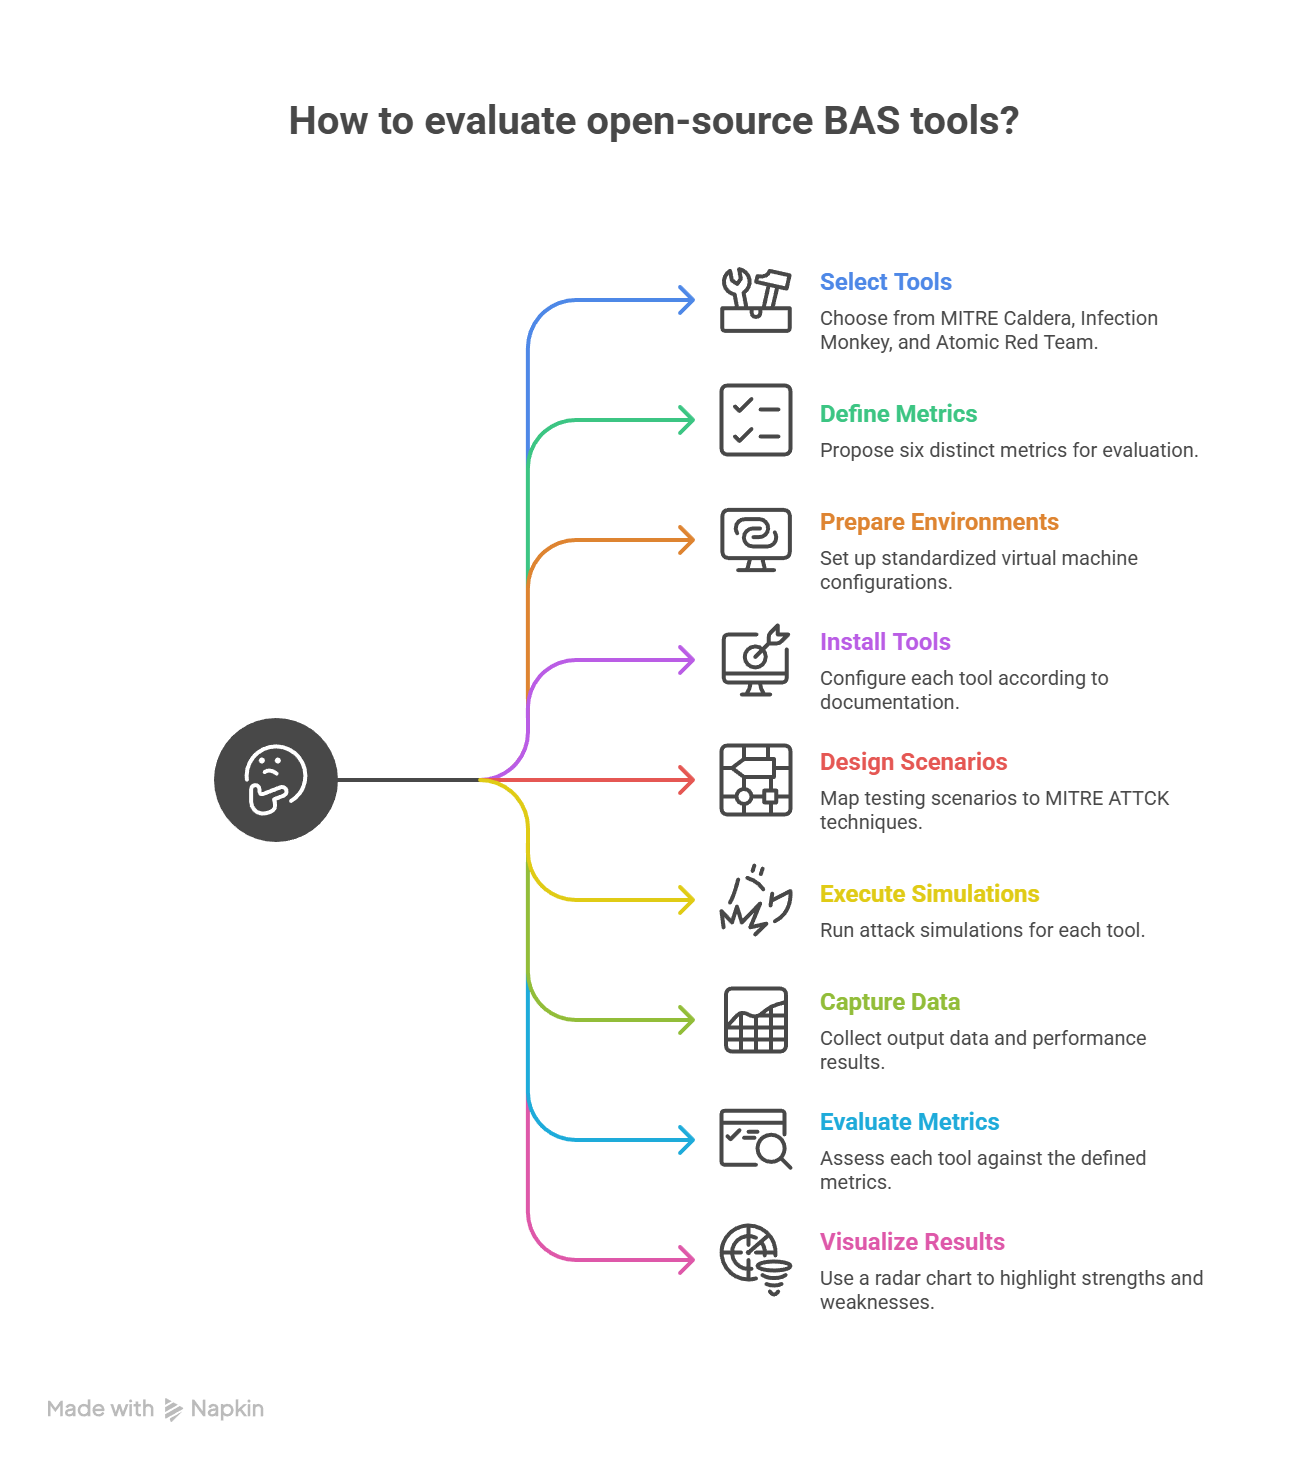
\includegraphics[width=1\linewidth]{figures/BAS-Research Workflow.png}
    \caption{Research Workflow}
    \label{fig:BAS-Research Workflow}
    \end{figure}

%--------------------|    3.2 Selection of Open-Source BAS Solutions    |-----------------------|
\section{Selection of Open-Source BAS Solutions}
The selection process for this research employed a systematic \textbf{down-selection methodology} to ensure the chosen candidates represent the "gold standard" of modern open-source Breach and Attack Simulation (BAS). The process was executed in two distinct phases. Phase 1 applied binary architectural criteria—automation capability, repository health, and MITRE ATT\&CK framework alignment—to remove tools incompatible with autonomous laboratory deployment. Phase 2 applied a weighted AI consensus ranking to confirm the selection of the three highest-quality candidates for physical laboratory testing.

\subsection{Phase 1: Scope Filtering (Binary Exclusion)}
This study began with the nine tools identified in the foundational work of Landauer et al. ~\cite{landauer2024}. To isolate platforms suitable for a high-fidelity laboratory environment, three \textbf{Inclusion Criteria} were applied to assess architectural viability:

\begin{itemize}
    \item \textbf{Automation Capability:} The tool must support autonomous, multi-stage attack emulation—where subsequent actions depend on the success of previous steps—rather than static infection simulation or manual per-step execution.
    \item \textbf{Active Repository Health:} The tool must have received community updates within the last 36 months to ensure compatibility with modern, patched Linux environments (specifically Ubuntu 22.04/24.04 LTS and recent Kernel versions).
    \item \textbf{Framework Alignment:} The tool must natively map its procedures to the MITRE ATT\&CK framework to ensure standardized, industry-relevant reporting.
\end{itemize}

\begin{figure}[htbp]
    \centering
    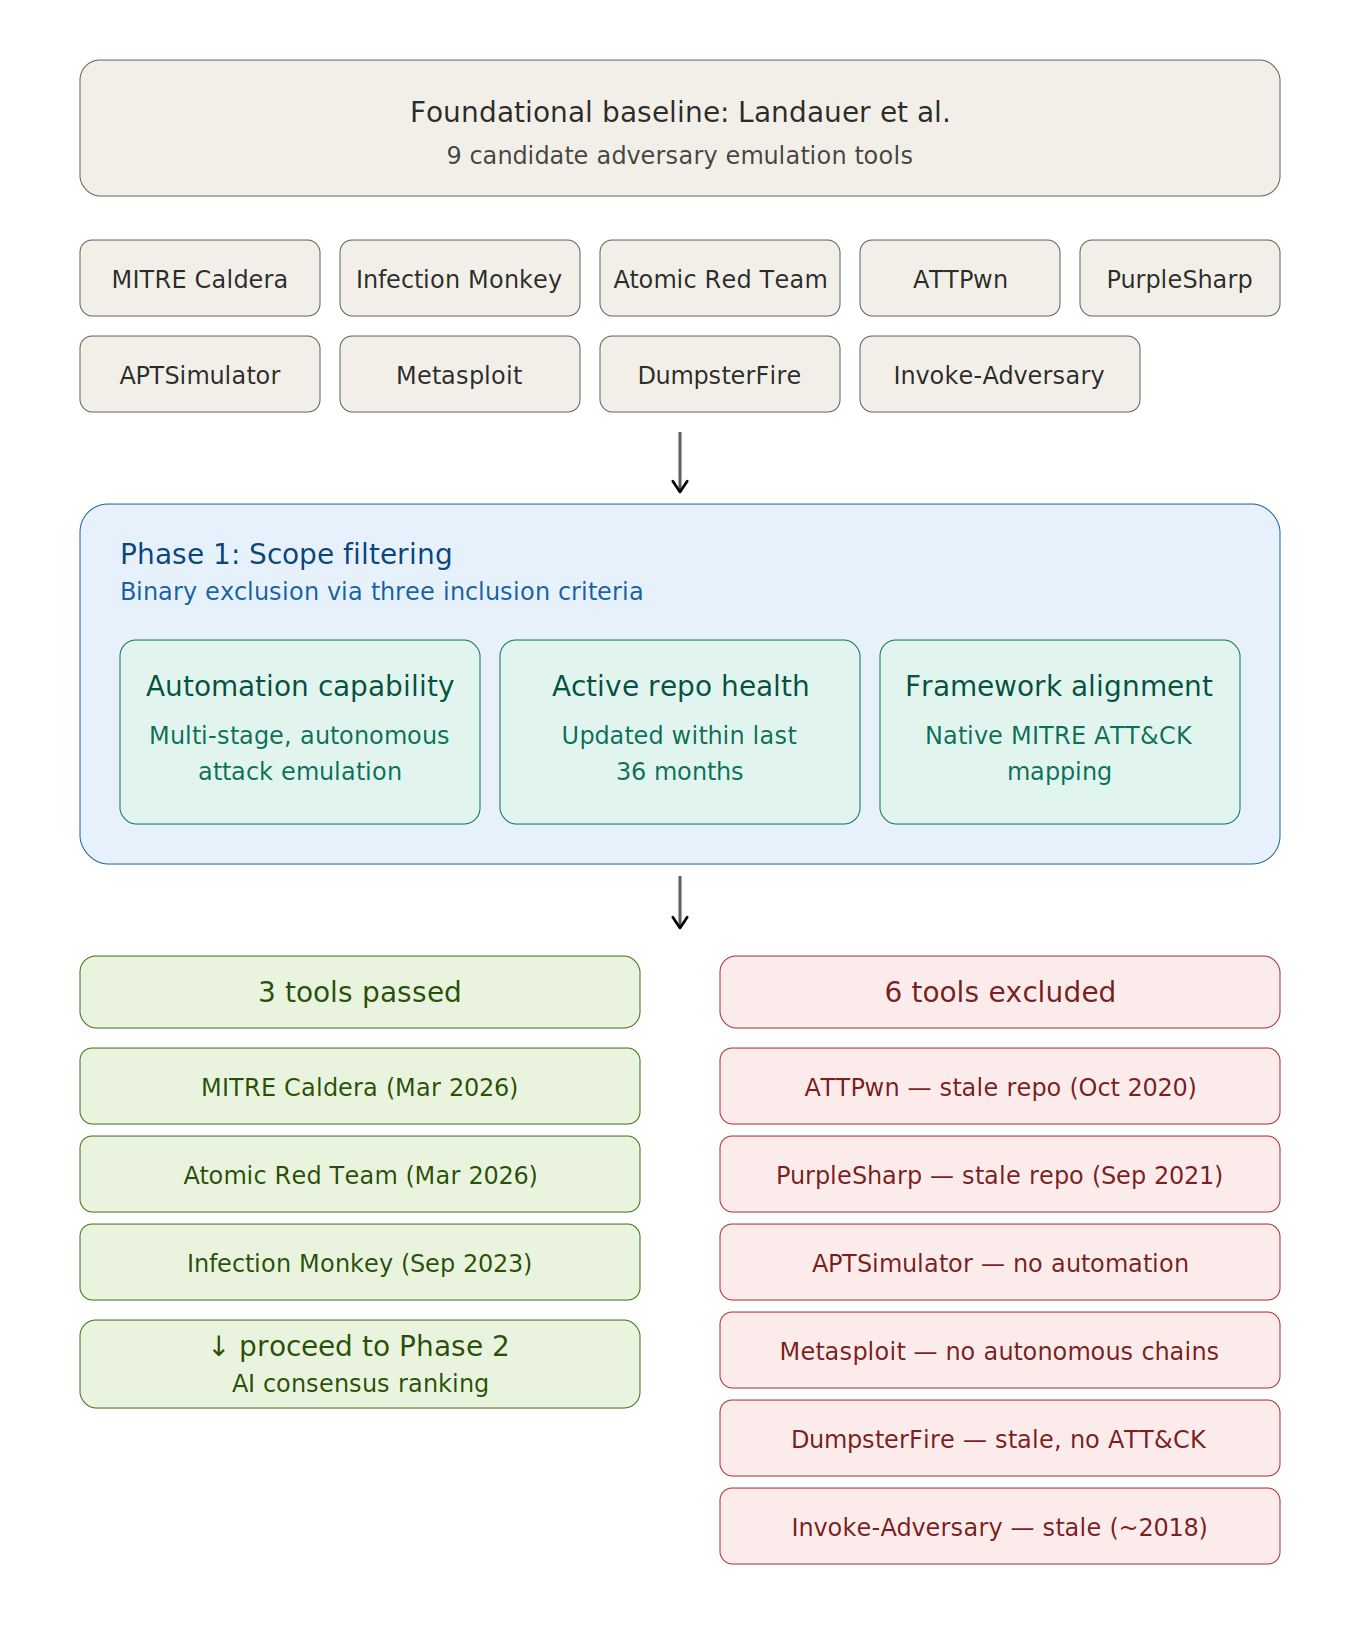
\includegraphics[width=1\linewidth]{figures/phase_1_scope_filtering.png}
    \caption{Scope filtering via binary exclusion.}
    \label{fig:Selection_phase1}
\end{figure}

As shown in Figure~\ref{fig:Selection_phase1}, application of the three criteria produced a clean partition of the candidate pool. The binary evaluation and current repository health of the initial tool pool are summarized in Table~\ref{tab:phase1_checklist}.

\begin{table}
    \centering
    \caption{Binary selection matrix for open-source BAS tools (Status: March 2026)}
    \label{tab:phase1_checklist}
    \renewcommand{\arraystretch}{1.4}
    \begin{tabular}{|l|c|c|c|c|c|}
        \hline
        \textbf{Tool Candidate} & \textbf{Automation} & \textbf{Repo Health} & \textbf{Last Update} & \textbf{Framework} & \textbf{Result} \\ \hline
        \textbf{MITRE Caldera}    & [Yes] & [Yes] & Mar 2026 & [Yes] & \textbf{PASS} \\ \hline
        \textbf{Infection Monkey} & [Yes] & [Yes] & Sep 2023 & [Yes] & \textbf{PASS} \\ \hline
        \textbf{Atomic Red Team}  & [Yes] & [Yes] & Mar 2026 & [Yes] & \textbf{PASS} \\ \hline
        ATTPwn                    & [Yes] & [No]  & Oct 2020 & [Yes] & FAIL \\ \hline
        PurpleSharp               & [Yes] & [No]  & Sep 2021 & [Yes] & FAIL \\ \hline
        APTSimulator              & [No]  & [Yes] & Jul 2023 & [Yes] & FAIL \\ \hline
        Metasploit                & [No]  & [Yes] & Mar 2026 & [Yes] & FAIL \\ \hline
        DumpsterFire              & [Yes] & [No]  & Dec 2017 & [No]  & FAIL \\ \hline
        Invoke-Adversary          & [Yes] & [No]  & $\sim$2018 & [Yes] & FAIL \\ \hline
    \end{tabular}
\end{table}

\noindent \textbf{Technical Justification for Inclusion:}
The following three tools—MITRE Caldera, Infection Monkey, and Atomic Red Team—successfully met all criteria. These platforms demonstrate the necessary architectural depth for empirical performance measurement on Ubuntu systems, supporting autonomous decision-making and active alignment with the MITRE ATT\&CK matrix.

\noindent \textbf{Technical Justification for Exclusion:}
Six tools were excluded due to specific architectural or maintenance limitations identified in Table~\ref{tab:phase1_checklist}:
\begin{itemize}
    \item \textbf{ATTPwn (Failed Repo Health):} Stagnant since October 2020. The repository is considered legacy and lacks the necessary updates to support modern MITRE ATT\&CK technique variations or current Ubuntu-based Python dependencies.
    \item \textbf{PurpleSharp (Failed Repo Health):} No significant updates since late 2021, exceeding the 36-month maintenance threshold. It relies on legacy .NET assemblies that exhibit limited compatibility with modern security orchestration requirements.
    \item \textbf{APTSimulator (Failed Automation):} Functions as a "static artifact creator" that drops fake registry keys and files; it does not execute real-time network traffic or process-level behaviors required for dynamic telemetry.
    \item \textbf{Metasploit (Failed Automation):} Although powerful, it is a manual penetration testing framework requiring human-in-the-loop operation; it lacks the autonomous planning engine required for automated BAS research.
    \item \textbf{DumpsterFire (Failed Health/Alignment):} Stagnant since 2017. It lacks native MITRE ATT\&CK mapping and exhibits significant dependency rot on modern Ubuntu kernels.
    \item \textbf{Invoke-Adversary (Failed Repo Health):} No significant updates in over 8 years. The repository is functionally incompatible with modern Ubuntu Python and PowerShell Core environments.
\end{itemize}

This filtering phase resulted in three primary candidates, which were then subjected to Phase 2 comparative ranking.

\subsection{Phase 2: Selection via AI Consensus Ranking (Weighted Evaluation)}
To finalize the selection, a triangulated AI evaluation was conducted using five independent artificial intelligence (AI) assistants: Gemini, ChatGPT, Copilot, Claude, and DeepAI. These models were tasked with ranking the three Phase 1 survivors against open-ended write-in alternatives, based on industry adoption, scenario extensibility, and documentation quality, as of May 2026. This open-ended formulation was deliberate: it allowed contemporary platforms outside the Landauer et al. baseline to surface as write-in candidates, providing a transparency check on whether any modern BAS tool had been overlooked by the foundational baseline.

\begin{figure}
    \centering
    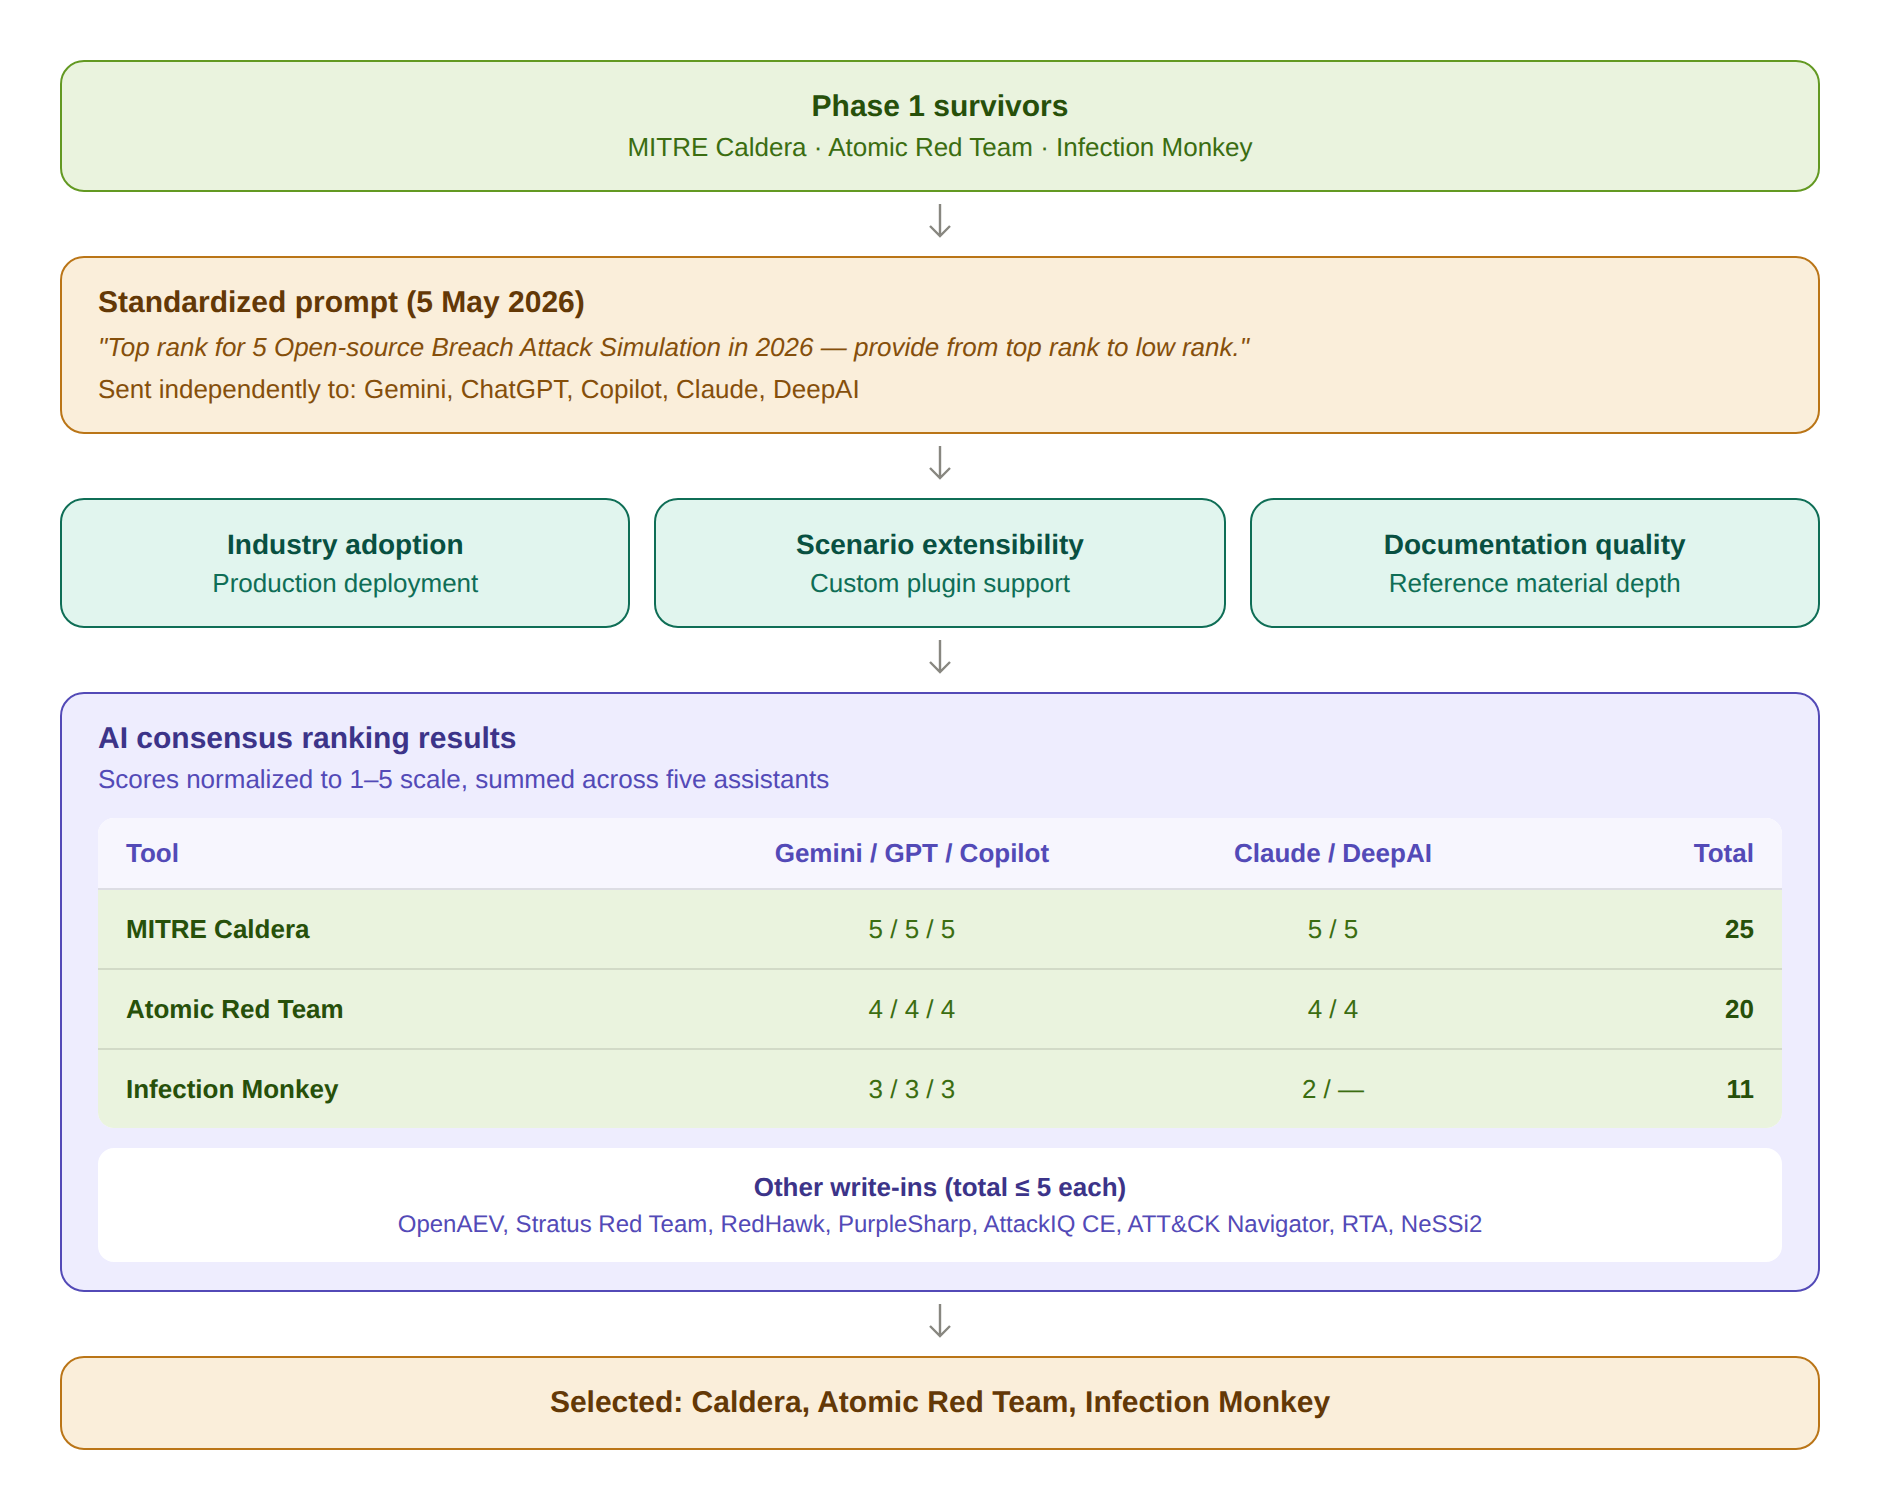
\includegraphics[width=1\linewidth]{figures/Select_Phase2.png}
    \caption{AI consensus ranking via weighted triangulation.}
    \label{fig:Selection_phase2}
\end{figure}

As showed in Figure~\ref{fig:Selection_phase2}, a point-based scoring system was applied (1st place = 5 points, 2nd place = 4 points, 3rd place = 3 points, etc.) to synthesize the rankings and mitigate individual model bias. The results of this process, summarized in Table~\ref{tab:bas_consensus}, consistently identified MITRE Caldera, Atomic Red Team, and Infection Monkey as the most highly ranked platforms.

\begin{table}
\centering
\caption{AI consensus ranking of open-source BAS candidates (5 May 2026)}
\label{tab:bas_consensus}
\renewcommand{\arraystretch}{1.25}
\begin{tabular}{l c c c c c >{\columncolor{lightgray}}c}
\toprule
\textbf{Tool Candidate} & \textbf{Gemini} & \textbf{ChatGPT} & \textbf{Copilot} & \textbf{Claude} & \textbf{DeepAI} & \textbf{Total Score} \\
\midrule
\textbf{MITRE Caldera}     & 5 & 5 & 5 & 5 & 5  & \textbf{25} \\
\textbf{Atomic Red Team}   & 4 & 4 & 4 & 4 & 4  & \textbf{20} \\
\textbf{Infection Monkey}  & 3 & 3 & 3 & 2 & -- & \textbf{11} \\
\midrule
OpenAEV            & 2  & -- & -- & 3  & -- & \textbf{5} \\
Stratus Red Team   & 1  & 2  & -- & 1  & -- & \textbf{4} \\
RedHawk            & -- & -- & -- & -- & 3  & \textbf{3} \\
PurpleSharp        & -- & -- & -- & -- & 2  & \textbf{2} \\
AttackIQ CE        & -- & -- & 2  & -- & -- & \textbf{2} \\
ATT\&CK Navigator  & -- & -- & -- & -- & 1  & \textbf{1} \\
RTA                & -- & 1  & -- & -- & -- & \textbf{1} \\
NeSSi2             & -- & -- & 1  & -- & -- & \textbf{1} \\
\bottomrule
\end{tabular}
\end{table}

Several write-in candidates were proposed by individual assistants, most notably OpenBAS/OpenAEV (rebranded by Filigran in November 2025), alongside Metasploit, Stratus Red Team, Prelude Operator, Purple Sharpie, AttackIQ, Red Team Tools, and Scythe. None of these accumulated more than four points across the panel, falling well short of the lowest-ranked Phase 1 survivor (Infection Monkey at 13 points). This substantial gap between the three Phase 1 survivors and the write-in tier provides triangulated validation that the foundational baseline of Landauer et al. continues to enclose the most defensible open-source BAS candidates as of April 2026.

\subsection{Selection Summary}
The triangulation process produced a clear hierarchy that was consistent across both phases. \textbf{MITRE Caldera} emerged as the primary candidate due to its sophisticated "Abilities and Adversaries" engine, which provides the deepest support for autonomous, multi-stage attack chains. \textbf{Atomic Red Team} was selected as the second-ranked platform, serving as the industry-standard library for atomic test execution and offering the broadest community-maintained ATT\&CK technique coverage. \textbf{Infection Monkey} was selected as the third candidate for its unique focus on automated lateral movement and network resilience testing, complementing the procedural depth of the other two platforms. Together, these three tools form the basis of the subsequent empirical evaluation in this research.

%-------------------------------|    3.3 Comparison matrix    |---------------------------------|
\section{Comparison Matrix}
To ensure the evaluation framework is both grounded in established academic standards and capable of addressing the critical research gaps identified in Chapter~2, the assessment of each open-source BAS tool is based on six criteria. The framework adopts a hybrid approach: several criteria are adapted directly from existing literature, while others are introduced by this study to measure practical operational realities that previous theoretical models omitted. The justification for each criterion is defined as follows:

\begin{enumerate}
    \item \textbf{Usability \& Deployment Complexity:} This criterion evaluates tool implementation friction by quantifying required installation steps and package dependencies. Addressing the high deployment complexity that often hinders open-source adoption, this criterion operationalizes the Installation \& Configuration category from Landauer et al.~\cite{landauer2024} into exact, laboratory-measured deployment parameters.

    \item \textbf{Threat Intelligence Alignment \& Maintenance:} This criterion assesses the frequency and automation of repository updates. Because stagnant tools quickly lose validation value against evolving threats, this criterion operationalizes the requirement for dynamic scenario feedback established by Wang et al.~\cite{wang2025} into a measurable assessment of how effectively a tool modernizes its attack library.

    \item \textbf{Scenario Coverage, Reliability \& Relevance:} This criterion adapts elements of the Features \& Capabilities category from Landauer et al.~\cite{landauer2024} (such as mapping to MITRE ATT\&CK) and integrates the necessity for multi-stage attack modeling established by Kuhl et al.~\cite{kuhl2007}. In addition, this study introduces an empirical reliability test that, to the author's knowledge, has not previously been applied to comparative evaluation of open-source BAS tools. Rather than relying on qualitative offline checklists or synthetic data, the introduced sub-criterion evaluates the tool's library alignment, indexed in this study as S1 through S20, and its empirical execution success rate in a live laboratory environment to ensure payloads run without crashing the target system.

    \item \textbf{Operational Performance \& Output Quality:} Previous academic models~\cite{wang2025,kuhl2007} did not address the computational cost of running simulation infrastructure. This study therefore introduces a performance criterion that records the BAS server's exact resource overhead (CPU and RAM) during active simulation. To isolate variables, execution is verified solely via native operating-system telemetry (e.g., Windows Event Logs, auditd). The criterion further evaluates the actionable quality of each tool's security reports, drawing on Roque et al.~\cite{roque2024}'s demonstration that report quality directly determines the value of simulation outcomes for downstream defensive tuning.

    \item \textbf{Framework Extensibility \& Custom Scenario Creation:} This criterion evaluates the technical difficulty of customizing TTPs or modifying attack chains. Grounded in the theoretical frameworks of Wang et al.~\cite{wang2025} and adapting specific elements from Landauer et al.~\cite{landauer2024}'s Features \& Capabilities category, it measures the tool's capacity to emulate highly specific, industry-relevant threat actors by quantifying the technical friction of custom payload creation (e.g., GUI/YAML editing versus core programming).

    \item \textbf{Community Health \& Project Maturity:} This criterion evaluates long-term project viability by measuring commit frequency and GitHub community metrics. Since open-source tools rely entirely on volunteer maintainers, abandoned projects pose significant operational risks. Adapted from the Community \& Support category of Landauer et al.~\cite{landauer2024}, this criterion translates qualitative community assessments into objective evaluations utilizing public repository data.
\end{enumerate}

By synthesizing existing literature with these new operational measurements, the resulting evaluation framework — operationalized in Section~\ref{sec:Scoring} as the Complete Evaluation Scoring Matrix (Table~\ref{tab:bas_evaluation_matrix_complete}) — facilitates a comprehensive, real-world assessment of each tool's capabilities.

%--------------------------------|    3.4 Comparison Matrix    |--------------------------------|
\section{Evaluation Scoring Matrix}\label{sec:Scoring}
This matrix provides a detailed breakdown of the scoring for each evaluation criterion on a 0–3 scale, enabling a clear and quantitative comparison of the open-source BAS tools. Scores are derived either from direct Experimental Data (Exp) gathered during laboratory simulations, or through Document and Online Searches (Search) for metrics evaluating project maturity. The final comparative results will be visually represented using a spider chart, illustrating the performance of each tool across the six metrics.


%###############| Complete Evaluation Scoring Matrix |##################
\begin{longtable}{|l|p{4cm}|p{8cm}|l|}
    \caption{Complete Evaluation Scoring Matrix}
    \label{tab:bas_evaluation_matrix_complete} \\
    \hline
    \textbf{ID} & \textbf{Criterion Description} & \textbf{Scoring Scale} & \textbf{Src} \\
    \hline
    \endfirsthead
    \hline
    \textbf{ID} & \textbf{Criterion Description} & \textbf{Scoring Scale} & \textbf{Src} \\
    \hline
    \endhead
    
    % --- SECTION 1 ---
    \multicolumn{4}{|l|}{\textbf{1. Usability \& Deployment Complexity}} \\
\hline
    1.1 & Number of installation steps required ~\cite{landauer2024} & 
    [3] Very Simple ($<$ 6 steps) \newline 
    [2] Standard (6--10 steps) \newline 
    [1] Complex (11--15 steps) \newline 
    [0] Too Complex ($>$ 15 steps) & Exp \\ \hline
    1.2 & Dependency requirements ~\cite{landauer2024} & 
    [3] Minimal ($<$ 2 packages) \newline 
    [2] Few (2--5 packages) \newline 
    [1] Heavy (6--15 packages) \newline 
    [0] Excessive ($>$ 15 packages) & Exp \\ \hline
    
    % --- SECTION 2 ---
    \multicolumn{4}{|l|}{\textbf{2. Threat Intelligence Alignment \& Maintenance}} \\
    \hline
    2.1 & Frequency of MITRE Attack techniques update ~\cite{wang2025} & 
    [3] Frequent (Weekly/Monthly) \newline 
    [2] Regular (Quarterly) \newline 
    [1] Rare (Annual or Irregular) \newline 
    [0] Static (No updates in $>$ 1 year) & Exp \\ \hline
    2.2 & Update method ~\cite{wang2025} & 
    [3] Synchronized (Immediate) \newline 
    [2] Scheduled (Automated) \newline 
    [1] Manual \newline 
    [0] No Update (Static) & Exp \\ \hline
    
    % --- SECTION 3 ---
    \multicolumn{4}{|l|}{\textbf{3. Scenario Coverage, Reliability \& Relevance}} \\
    \hline
    3.1 & Number of supported MITRE ATT\&CK techniques (of 697 valid v19.2 techniques)~\cite{landauer2024,kuhl2007} &
    [3] High ($>$ 348 techniques, $>$50\%) \newline
    [2] Moderate (174--348 techniques, 25--50\%) \newline
    [1] Low (70--174 techniques, 10--25\%) \newline
    [0] Minimal ($<$ 70 techniques, $<$10\%) & Exp \\ \hline
    3.2 & High-Probability Threat Alignment & 
    [3] High Alignment (Over 80\% coverage; 16--20 of 20) \newline 
    [2] Moderate Alignment (50\%--79\% coverage; 10--15 of 20) \newline 
    [1] Inadequate (1\%--49\% coverage; 1--9 of 20) \newline 
    [0] None (0\% coverage) & Exp \\ \hline
    3.3 & Execution reliability & 
    [3] Highly Reliable ($>$ 75\% success rate) \newline 
    [2] Consistent (50\%--75\% success rate) \newline 
    [1] Unstable (1\%--49\% success rate) \newline 
    [0] Failed (0\% success rate) & Exp \\ \hline
    
    % --- SECTION 4 - Operational Performance \& Output Quality ---
    \multicolumn{4}{|l|}{\textbf{4. Operational Performance \& Output Quality}} \\
    \hline
    4.1 & CPU usage of BAS server & 
    [3] Minimal ($<$ 15\% overhead) \newline 
    [2] Moderate (15\%--40\% overhead) \newline 
    [1] Heavy ($>$ 40\% overhead) \newline 
    [0] Unstable (Crashes or unresponsive under load) & Exp \\ \hline
    4.2 & Memory usage of BAS server &  
    [3] Minimal ($<$ 15\% overhead) \newline 
    [2] Moderate (15\%--40\% overhead) \newline 
    [1] Heavy ($>$ 40\% overhead) \newline 
    [0] Unstable (OOM termination under load) & Exp \\ \hline
    4.3 & Quality of reports ~\cite{roque2024} & 
    [3] Actionable (Detailed with fix scripts/rules) \newline 
    [2] General Advice (Logs with interpretation) \newline 
    [1] Result Only (Pass/Fail) \newline 
    [0] No Reports (CLI output only) & Exp \\ \hline
    
    % --- SECTION 5 ---
    \multicolumn{4}{|l|}{\textbf{5. Framework Extensibility \& Custom Scenario Creation}} \\
    \hline
    5.1 & Add/modify attack scenarios~\cite{landauer2024,wang2025} & 
    [3] Easy (Templates/GUI) \newline 
    [2] Possible (Code required) \newline 
    [1] Very Limited \newline 
    [0] Not Supported & Exp \\ \hline
    5.2 & Ease of creating custom TTPs ~\cite{landauer2024,wang2025} & 
    [3] User-Friendly (Built-in modularity) \newline 
    [2] Requires Scripting \newline 
    [1] Complex/Undocumented \newline 
    [0] Not Supported & Exp \\ \hline
    
    % --- SECTION 6 - Community Health \& Project Maturity ---
    \multicolumn{4}{|l|}{\textbf{6. Community Health \& Project Maturity}} \\
    \hline
    6.1 & Frequency of commits/updates~\cite{landauer2024} & 
    [3] Active (commits within 6 months) \newline 
    [2] Updates (commits within 6--12 months) \newline 
    [1] Stalled (last commit 12--24 months ago) \newline 
    [0] Abandoned (no commits in > 24 months) & Search \\ \hline
    6.2 & Community activity~\cite{landauer2024} & 
    [3] Large/Active (Top 25\%) \newline 
    [2] Moderate Presence (Middle 50\%) \newline 
    [1] Small/Inactive (Bottom 25\%) \newline 
    [0] No Community & Search \\ \hline
\end{longtable}

\noindent The detailed scoring criteria for each metric presented in Table \ref{tab:bas_evaluation_matrix_complete} are outlined below:

\begin{description}
    \item[1. Usability \& Deployment Complexity] \hfill \par
    \textbf{1.1 Installation Steps}
    \begin{itemize}
        \item \textbf{[3] Very Simple ($<$ 6 steps):} Characterized by one-click, automated, or single-binary setups requiring minimal manual configuration.
        \item \textbf{[2] Standard (6--10 steps):} Represents average deployment efforts, involving typical tasks such as setting environment variables or basic directory setups.
        \item \textbf{[1] Complex (11--15 steps):} Indicates high setup friction requiring manual service linking or multi-stage initializations.
        \item \textbf{[0] Too Complex ($>$ 15 steps):} Denotes excessive, labor-intensive, and error-prone setup requirements.
    \end{itemize}
    \textbf{1.2 Dependency Requirements}
    \begin{itemize}
        \item \textbf{[3] Minimal ($<$ 2 packages):} Characterized by self-contained tools or those utilizing native operating system utilities exclusively.
        \item \textbf{[2] Few (2--5 packages):} Requires common runtime environments (e.g., Python or Docker) easily obtainable from standard repositories.
        \item \textbf{[1] Heavy (6--15 packages):} Necessitates complex application stacks, including specific database versions, multiple runtimes, or specialized web servers.
        \item \textbf{[0] Excessive ($>$ 15 packages):} Involves highly complex dependency chains with a high risk of version conflicts.
    \end{itemize}

    \item[2. Threat Intelligence Alignment \& Maintenance] \hfill \par
    \textbf{2.1 Frequency of MITRE ATT\&CK techniques update}
    \begin{itemize}
        \item \textbf{[3] Frequent (Weekly/Monthly):} Indicates highly active repositories that maintain immediate alignment with newly published CVEs and adversarial behaviors.
        \item \textbf{[2] Regular (Quarterly):} Reflects consistent, stable release cycles for threat content.
        \item \textbf{[1] Rare (Annual or Irregular):} Denotes sporadic updates, significantly increasing the risk of failing to capture emerging threats.
        \item \textbf{[0] Static (No updates in $>$ 1 year):} Suggests the project is likely discontinued or abandoned.
    \end{itemize}
    \textbf{2.2 Update Method}
    \begin{itemize}
        \item \textbf{[3] Synchronized (Immediate):} Features automated mechanisms that synchronize new threat data immediately upon release to the central repository.
        \item \textbf{[2] Scheduled (Automated):} Employs predetermined, automated schedules, allowing for controlled environment changes.
        \item \textbf{[1] Manual:} Requires manual intervention, such as downloading and executing update scripts or configuration files.
        \item \textbf{[0] No Update (Static):} Lacks functional update mechanisms, requiring complete re-installation to acquire new threat content.
    \end{itemize}

\item[3. Scenario Coverage, Reliability \& Relevance] \hfill \par
    \textbf{3.1 Number of supported MITRE ATT\&CK techniques}
    The denominator for this criterion is the MITRE ATT\&CK Enterprise
    matrix, version 19.2 (222 top-level techniques plus 475 sub-techniques,
    downloaded directly from
    \url{https://attack.mitre.org/docs/attack-excel-files/v19.2/enterprise-attack/enterprise-attack-v19.2-techniques.xlsx}
    on 7 September 2026), for a total of 697 valid, non-deprecated
    techniques. Each tool's numerator counts only the technique identifiers
    it claims that still exist under that exact identifier in v19.2;
    identifiers that MITRE has since deprecated, merged, or renumbered
    (for example, the entire \texttt{T1562} ``Impair Defenses'' family was
    renumbered to \texttt{T1685} in ATT\&CK v19) are excluded, since they no
    longer represent a technique the tool can be credited with covering
    under the current framework.
    \begin{itemize}
        \item \textbf{[3] High ($>$348 techniques):} Covers more than 50\% of
              the 697-technique v19.2 baseline, providing extensive reach
              across the full adversarial kill chain and nearly all ATT\&CK
              tactic phases.
        \item \textbf{[2] Moderate (174--348 techniques):} Covers 25--50\% of
              the v19.2 baseline, establishing a solid baseline that
              encompasses the most prevalent adversarial tactics and supports
              meaningful multi-phase scenario construction.
        \item \textbf{[1] Low (70--174 techniques):} Covers 10--25\% of the
              v19.2 baseline, affording limited breadth primarily
              concentrated in specialist tactic areas; suitable for focused
              rather than comprehensive security validation.
        \item \textbf{[0] Minimal ($<$70 techniques):} Covers less than
              10\% of the v19.2 baseline; deemed inadequate for
              broad adversary emulation or cross-tactic comparative evaluation.
    \end{itemize}

    \textbf{3.2 High-Probability Threat Alignment} \hfill \par
    Evaluates the tool's inclusion of the most frequently observed techniques in real-world breaches (e.g., Top 20 techniques identified in MITRE Center for Threat Informed Defense (CTID)).
    \begin{itemize}
        \item \textbf{[3] High Alignment ($\ge$ 80\% coverage):} The tool successfully supports 16 to 20 of the prioritized techniques, making it highly effective for targeted threat actor emulation.
        \item \textbf{[2] Moderate Alignment (50\%--79\% coverage):} The tool covers 10 to 15 techniques, providing a solid baseline but lacking specialized advanced procedures.
        \item \textbf{[1] Inadequate (1\%--49\% coverage):} The tool covers 9 or fewer techniques, meaning it is blind to the vast majority of the critical threats identified for the region.
        \item \textbf{[0] None (0\% coverage):} Offers zero support for the specific critical techniques selected for this study.
    \end{itemize}
    
    \textbf{3.3 Execution reliability} \hfill \par
    Success rate is calculated based on the successful technical execution of the payload without crashing, excluding intended defensive blocks.
    \begin{itemize}
        \item \textbf{[3] Highly Reliable ($>$ 75\% success rate):} Demonstrates consistent execution workflows without recurring technical errors or crashes.
        \item \textbf{[2] Consistent (50\%--75\% success rate):} Exhibits mostly stable execution, interrupted only by occasional, non-critical errors.
        \item \textbf{[1] Unstable (1\%--49\% success rate):} Experiences significant technical noise or errors that frequently interrupt the simulation workflow.
        \item \textbf{[0] Failed (0\% success rate):} Consistently crashes or completely fails to execute the defined attack scenarios.
    \end{itemize}

    \item[4. Operational Performance \& Output Quality]  \hfill \par
    Resource overhead is calculated relative to the server's baseline idle resource usage prior to initiating concurrent attack simulations.

    \textbf{4.1 CPU Usage of BAS Server}
    \begin{itemize}
        \item \textbf{[3] Minimal ($<$ 15\% overhead):} Demonstrates highly optimized processing. The C2 server imposes negligible system impact during active campaign execution.
        \item \textbf{[2] Moderate (15\%--40\% overhead):} Reflects acceptable processing loads typical of heavier Java or Python-based application stacks orchestrating concurrent tasks.
        \item \textbf{[1] Heavy ($>$ 40\% overhead):} Generates significant, inefficient CPU spikes that actively monopolize resources and could degrade co-located enterprise services.
        \item \textbf{[0] Unstable:} Uncapped CPU overhead leading to server crashes, timeouts, or complete unresponsiveness.
    \end{itemize}
    \textbf{4.2 Memory Usage of BAS Server}
    \begin{itemize}
        \item \textbf{[3] Minimal ($<$ 15\% overhead):} Demonstrates highly efficient memory allocation and garbage collection during active simulation tracking.
        \item \textbf{[2] Moderate (15\%--40\% overhead):} Exhibits standard RAM consumption expected from a web-backend maintaining active agent connections.
        \item \textbf{[1] Heavy ($>$ 40\% overhead):} Manifests a bloated memory footprint resulting in system paging or severe host performance degradation.
        \item \textbf{[0] Unstable:} Severe memory leaks leading to exhaustion (Out-Of-Memory/OOM events), terminating core processes or destabilizing the server.
    \end{itemize}
    \textbf{4.3 Quality of Reports}
    \begin{itemize}
        \item \textbf{[3] Actionable:} Provides specific remediation guidance, including outputs containing Snort rules, Sigma rules, or EDR fix scripts.
        \item \textbf{[2] General Advice:} Offers contextual interpretation and high-level recommendations for mitigating identified vulnerabilities.
        \item \textbf{[1] Result Only:} Outputs binary outcomes consisting of simple Pass/Fail summaries without contextual data.
        \item \textbf{[0] No Reports:} Lacks reporting functionality entirely, providing only raw command-line terminal output.
    \end{itemize}

    \item[5. Framework Extensibility \& Custom Scenario Creation]  \hfill \par
    \textbf{5.1 Add/Modify Attack Scenarios}
    \begin{itemize}
        \item \textbf{[3] Easy (Templates/GUI):} Facilitated by simple YAML/JSON files or visual interfaces for editing scenarios.
        \item \textbf{[2] Possible (Code required):} Modification is supported but demands specific programming proficiency (e.g., Python, Ruby).
        \item \textbf{[1] Very Limited:} Features undocumented customization that only permits the modification of built-in parameters.
        \item \textbf{[0] Not Supported:} Operates as a closed framework with no mechanism to modify core attack logic.
    \end{itemize}
    \textbf{5.2 Ease of Creating Custom TTPs}
    \begin{itemize}
        \item \textbf{[3] User-Friendly:} Incorporates built-in modularity, drag-and-drop features, or intuitive scripting to chain complex sequences and kill chains.
        \item \textbf{[2] Requires Scripting:} Chaining is permissible but necessitates complex, manual scripting by the operator.
        \item \textbf{[1] Complex/Undocumented:} Lacks formal chaining support; simulating multi-stage attacks requires major core modifications.
        \item \textbf{[0] Not Supported:} Actions are strictly isolated; the tool is incapable of linking operations into a coordinated scenario.
    \end{itemize}

    \item[6. Community Health \& Project Maturity]  \hfill \par
    \textbf{6.1 Frequency of Commits/Updates}
    \begin{itemize}
        \item \textbf{[3] Active ($<$ 6 months):} Repository exhibits recent developer commits and regular bug fixes.
        \item \textbf{[2] Updates ($<$ 12 months):} Represents stable projects that receive patches on a less frequent but consistent basis.
        \item \textbf{[1] Stalled ($>$ 1 year):} Indicates dormant repositories where active development has evidently stalled.
        \item \textbf{[0] Abandoned ($>$ 2 years):} Characterizes officially discontinued projects with no commits for over two years.
    \end{itemize}
    \textbf{6.2 Community Activity}
    \begin{itemize}
        \item \textbf{[3] Large/Active (Top 25\%):} Characterized by high popularity, thousands of GitHub stars, extensive forks, and a massive contributor base (e.g., Metasploit level).
        \item \textbf{[2] Moderate Presence (Middle 50\%):} Maintains a stable user base with periodic community interactions and documented forks.
        \item \textbf{[1] Small/Inactive (Bottom 25\%):} Exhibits very few contributors, low watcher counts, and minimal evidence of broader adoption.
        \item \textbf{[0] No Community:} Demonstrates zero public repository metrics, lacks forums, and offers no maintainer support.
    \end{itemize}
\end{description}

%#######################################################################################%
%######################|          3.5  Testing Scenarios}         |#####################%
%#######################################################################################%

\section{Testing Scenarios}\label{sec:Scenarios}

The experimental setting for this research involves deploying selected Breach and Attack Simulation (BAS) tools within controlled, isolated virtual environments designed to reflect typical enterprise network constraints. All tests are performed on Linux-based virtual machines to ensure consistency and reproducibility. Each tool is installed according to official documentation, and all configurations strictly adhere to recommended setup parameters to avoid external biases.

\begin{itemize}
    \item \textbf{Testing Procedure}

    The procedure for each BAS tool follows these systematic steps:

\begin{enumerate}
    \item \textbf{Installation:} The tool is installed and configured in the test environment, including server setup and agent deployment across target systems.
    \item \textbf{Execute Attack Simulation:} Carefully curated attack scenarios—mapped to the MITRE ATT\&CK framework—are launched, emulating adversary tactics and techniques to assess detection and defensive capabilities.
    \item \textbf{Capture Results:} All outputs, logs, and generated reports are collected, ensuring detailed documentation of each attack vector and the tool's response.
    \item \textbf{Evaluation:} Performance is measured and scored using the six proposed comparison metrics: usability and deployment complexity, threat intelligence alignment and maintenance, scenario coverage and execution reliability, operational performance and output quality, framework extensibility and custom scenario creation, and community health and project maturity.
\end{enumerate}
\begin{figure}
    \centering
    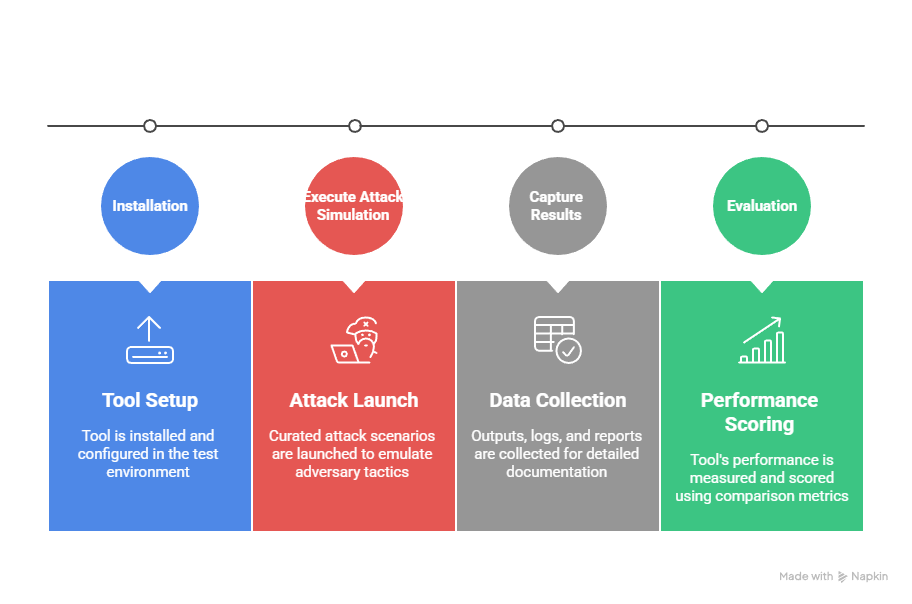
\includegraphics[width=1\linewidth]{figures/BAS-Testing Procedure - visual.png}
    \caption{Testing Procedure}
    \label{fig:Testing_Procedure}
\end{figure}

\noindent Figure~\ref{fig:Testing_Procedure} outlines the systematic four-phase methodology employed to evaluate the BAS tools. The process proceeds sequentially through: (1) Tool Setup, involving the installation and configuration of the test environment; (2) Attack Launch, where curated scenarios based on MITRE ATT\&CK are executed to emulate adversary tactics; (3) Data Collection, which captures comprehensive logs and tool outputs; and (4) Performance Scoring, where the gathered data is analyzed against six defined metrics to derive a final comparative assessment.
\end{itemize}
 % Research Methodology > Proposed Method
%==============================================================================%
%=========================|     CHAPTER 4 Experiment    |===========================%
%==============================================================================%

\chapter{EXPERIMENT AND PRELIMINARY RESULTS} \label{chap:experiment}
This chapter details the experimental implementation of the comparative study. It outlines the laboratory setup, installation, and execution of attack simulations using MITRE Caldera, Infection Monkey, and Atomic Red Team.

%#####################|    4.1     |############################%
\section{Hardware and Software Specifications}\label{sec:Specifications}
The experimental environment utilized a virtualized infrastructure to model a realistic enterprise network. The following specifications ensure the reproducibility of the simulations.
\begin{itemize}
\item \textbf{Infrastructure and Virtualization}
A high-performance physical host was used to run the virtual machines (VMs) concurrently. Table~\ref{tab:host_specs} details the hardware baseline.
\begin{table}[h]
    \centering
    \caption{Physical Host Machine Specifications}
    \label{tab:host_specs}
    \renewcommand{\arraystretch}{1.3}
    \begin{tabular}{l l}
    \toprule
    \textbf{Component} & \textbf{Specification} \\ 
    \midrule
    Processor (CPU) & Intel Core i5-10400 @ 2.90GHz \\
    Memory (RAM) & 32 GB \\
    Operating System & Windows 11 Pro \\
    Hypervisor & VMware Workstation 17 Pro \\
    \bottomrule
    \end{tabular}
\end{table}
\noindent The lab was divided into a \textbf{BAS Host} (C2 server) and a \textbf{Clients} (Victim). Their resource allocations are shown in Table~\ref{tab:vm_specs}.
\begin{table}
    \centering
    \caption{Virtual Machine Allocations}
    \label{tab:vm_specs}
    \renewcommand{\arraystretch}{1.2}
    \begin{tabularx}{\textwidth}{l c c c X}
    \toprule
    \textbf{Configuration} & \textbf{vCPU} & \textbf{RAM} & \textbf{Disk} & \textbf{Operating System} \\ 
    \midrule
    \textbf{Server / BAS Host} & 4 & 8 GB & 60 GB & Ubuntu 24.04 LTS \\
    \textbf{Client / Target} & 2 & 2 GB & 60 GB & Windows 11 Pro, Ubuntu 24.04 LTS \\
    \bottomrule
    \end{tabularx}
\end{table}

\item \textbf{Software Frameworks and Dependencies}

The BAS tools were configured according to their specific environmental needs on Ubuntu 24.04. Table~\ref{tab:software_versions_grouped} summarizes the software versions used for each tool.

% Define the 'L' column type (Left-aligned, auto-width)
\newcolumntype{L}{>{\raggedright\arraybackslash}X}

\begin{table}
    \centering
    \caption{Software and Framework Versions by Tool}
    \label{tab:software_versions_grouped}
    \renewcommand{\arraystretch}{1.3}
    \begin{tabularx}{\textwidth}{L L L}
    \toprule
    \textbf{Tool name} & \textbf{Component} & \textbf{Version / Environment} \\ 
    \midrule
    % FIX 1: Added "{3}{=}" -> Spans 3 rows, inherits column width (=)
    \multirow{3}{=}{\textbf{MITRE Caldera}} & Core Framework & 5.3.0 (Python 3.12.3) \\
     & Package Manager & Pip 24.0 \\
     & Front-end Engine & Node.js 22.21.0 \\
    \midrule
    % FIX 2: Added "{2}{=}" -> Spans 2 rows
    \multirow{2}{=}{\textbf{Infection Monkey}} & Island C2 Server & 2.3.0 (Linux AppImage) \\
     & Compatibility & libfuse2t64 (Legacy FUSE) \\
    \midrule
    % FIX 3: Added "{3}{=}" -> Spans 3 rows
    \multirow{3}{=}{\textbf{Atomic Red Team}} & Execution Engine & Invoke-AtomicRedTeam 2.1.0 \\
     & Runtime & PowerShell Core 7.5.4 \\
     & Parser & powershell-yaml 0.4.12 \\
    \bottomrule
    \end{tabularx}
\end{table}

\end{itemize}

%###################|          4.2          |############################%
\section{Installation}\label{sec:Installation}

The experimental infrastructure was deployed using a standardized strategy to ensure consistency across all test environments, moving from base preparation to tool-specific deployment.

%% --- SECTION 1: VM PREPARATION ---

\subsection{VM Preparation}

The first phase established a stable and reproducible foundation for the testing environment by creating a “Golden Image” base server. A single Ubuntu Server 24.04 LTS virtual machine was provisioned as the baseline platform and pre-configured with the shared dependencies required across all three BAS tools, ensuring consistency and simplifying later comparisons.
    \begin{itemize}
        \item \textbf{OS Installation:} Ubuntu Server (24.04 LTS) was installed to prioritize stability and resource efficiency.
        \item \textbf{System Updates:} The operating system repositories were synchronized, and all default packages were upgraded to their latest stable versions:
            \begin{lstlisting}
                $ sudo apt update && sudo apt upgrade
            \end{lstlisting}
        \item \textbf{Server Replication:} The base image was replicated to create three distinct BAS servers. A "Full Clone" method was utilized to ensure the virtual machines functioned as independent entities. Post-cloning, the \textbf{Hostname} for each server was modified to reflect its specific role. This was achieved using the following sequence:
            \begin{lstlisting}
                $ sudo hostnamectl set-hostname NEW_HOSTNAME
                $ sudo reboot
                $ sudo nano /etc/hosts
            \end{lstlisting}

    The manual edit of the \texttt{/etc/hosts} file was required to map the loopback address (\texttt{127.0.1.1}) to the new hostname, preventing resolution delays and ensuring internal services could correctly identify the local node.
    \end{itemize}

\subsection{Victim Preparation} 
    To simulate a realistic enterprise network comprising both user workstations and server workloads, two distinct victim virtual machines were provisioned:

    \begin{itemize}
        \item \textbf {Windows Victim (User Endpoint):} A dedicated Windows 11 Pro (24H2) virtual machine was configured to represent a typical employee workstation.
        \begin{itemize}
            \item \textbf{System Baselining:} The OS was updated to the latest build to ensure a modern security posture.
            \item \textbf{Network Configuration:} Static IP assignment was configured to ensure persistent connectivity between the BAS Host and the Client.
            \item \textbf{Defensive Baseline:} Microsoft Defender Antivirus was kept in its default state to measure the efficacy of standard built-in security controls.
        \end{itemize}

        \item \textbf {Linux Victim (Server Infrastructure):} An Ubuntu Server 22.04 LTS virtual machine was provisioned to represent critical infrastructure targets (e.g., Web/Database servers).
        \begin{itemize}
            \item \textbf{System Baselining:} The kernel and packages were updated to the latest stable release. Essential dependencies for BAS agents (Python 3, PowerShell for Linux, and Curl) were pre-installed to facilitate the execution of atomic tests.
            \item \textbf{Network Configuration:} A static IP was assigned to ensure reliable C2 connectivity. Additionally, the SSH service (Port 22) was enabled and configured to allow password authentication, creating a viable pathway for testing lateral movement scenarios (S11).
            \item \textbf{Defensive Baseline:} The standard Linux auditing framework (\texttt{auditd}) was installed and enabled with default rules to establish a detection baseline. AppArmor was left in its default ``Enforcing'' mode to measure the efficacy of out-of-the-box mandatory access controls.
        \end{itemize}
    \end{itemize}


%% --- SECTION 2: MITRE CALDERA ---
\subsection{MITRE Caldera 's Installation \& Configuration}

The installation of MITRE Caldera necessitated a dual-stack configuration to support both the Python back-end and the VueJS-based ``Magma'' front-end. This process involved significantly more steps than comparable tools due to dependency management on modern Linux systems.

\begin{itemize}
    \item \textbf{Source Control:} The source code was acquired by recursively cloning the official repository to ensure all mandatory plugin submodules were retrieved.
    
    \begin{lstlisting}[language=bash, caption={Repository Acquisition}]
$ sudo apt install git                  # Step 1 [Pkg 1]
$ git clone https://github.com/mitre/caldera.git --recursive # Step 2
$ cd caldera                            # Step 3
    \end{lstlisting}

    \item \textbf{Environment Isolation:} To comply with the externally-managed-environment policy enforced by Ubuntu 24.04, a Python virtual environment was required. As illustrated in Figure \ref{fig:venv-error}, modern Linux distributions protect system integrity by blocking direct \texttt{pip} installations into the system root.
    
    \begin{figure}
        \centering
        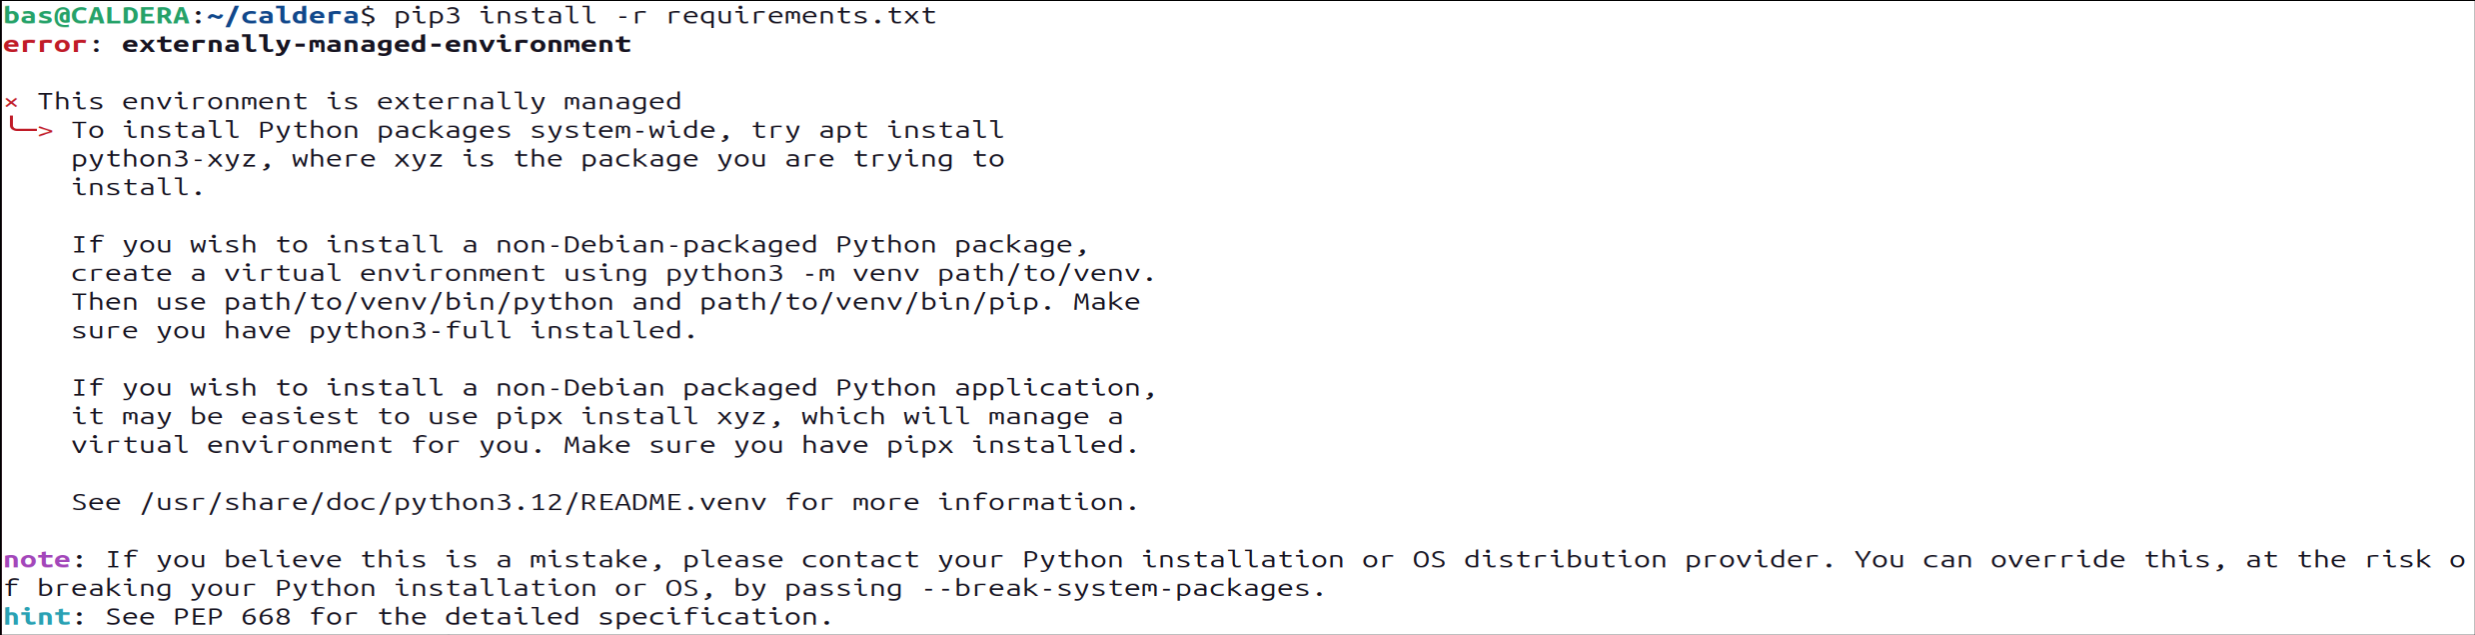
\includegraphics[width=1\textwidth]{figures/Caldera_error.png}
        \caption{Terminal output showing the \texttt{externally-managed-environment} error.}
        \label{fig:venv-error}
    \end{figure}

    \begin{lstlisting}[language=bash, caption={Python Virtual Environment Setup}]
$ sudo apt install python3-pip          # Step 4 [Pkg 2]
$ sudo apt install python3-venv         # Step 5 [Pkg 3]
$ python3 -m venv venv                  # Step 6
$ source venv/bin/activate              # Step 7
$ pip3 install -r requirements.txt      # Step 8
    \end{lstlisting}

    \item \textbf{Build Toolchain Upgrade:} The default Node.js repositories were insufficient for the Vite 7 build engine required by Caldera. The environment was manually upgraded to v22.x to meet the minimum requirement (\texttt{v22.12+}).
    
    \begin{lstlisting}[language=bash, caption={Node.js Toolchain Upgrade}]
$ rm -rf plugins/magma/node_modules     # Step 9
$ sudo apt install curl                 # Step 10 [Pkg 4]
$ curl -fsSL https://deb.nodesource.com/setup_22.x | sudo -E bash - # Step 11
$ sudo apt install npm                  # Step 12 [Pkg 5]
$ sudo apt install -y nodejs            # Step 13 [Pkg 6]
    \end{lstlisting}

    \item \textbf{Execution and Verification:} Finally, the server was compiled and launched to initialize the C2 service.
    
    \begin{lstlisting}[language=bash, caption={Server Compilation and Launch}]
$ python3 server.py --insecure --build  # Step 14
    \end{lstlisting}

    The successful completion of this deployment is confirmed in Figure \ref{fig:caldera_success_install} by the status message ``All systems ready.''
    
    \begin{figure}
        \centering
        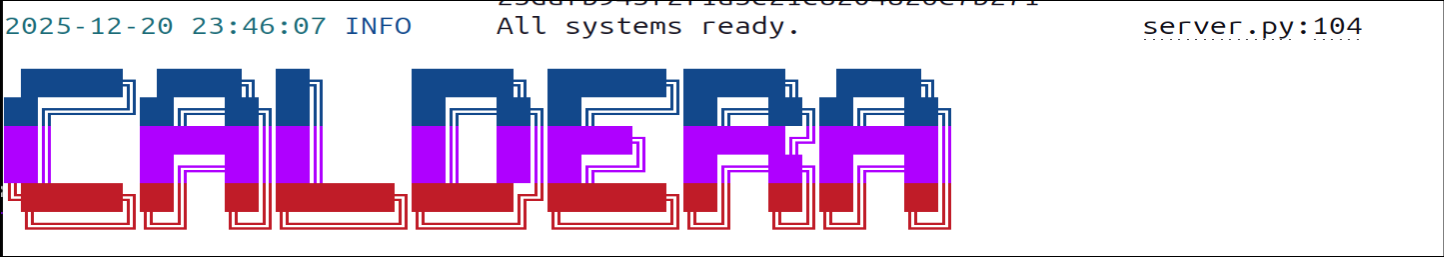
\includegraphics[width=1\textwidth]{figures/caldera_success_install.png}
        \caption{Successful server initialization and build output.}
        \label{fig:caldera_success_install}
    \end{figure}

    The final operational state is confirmed when the administrative login portal becomes accessible (Figure \ref{fig:caldera-interface}).

    \begin{figure}
        \centering
        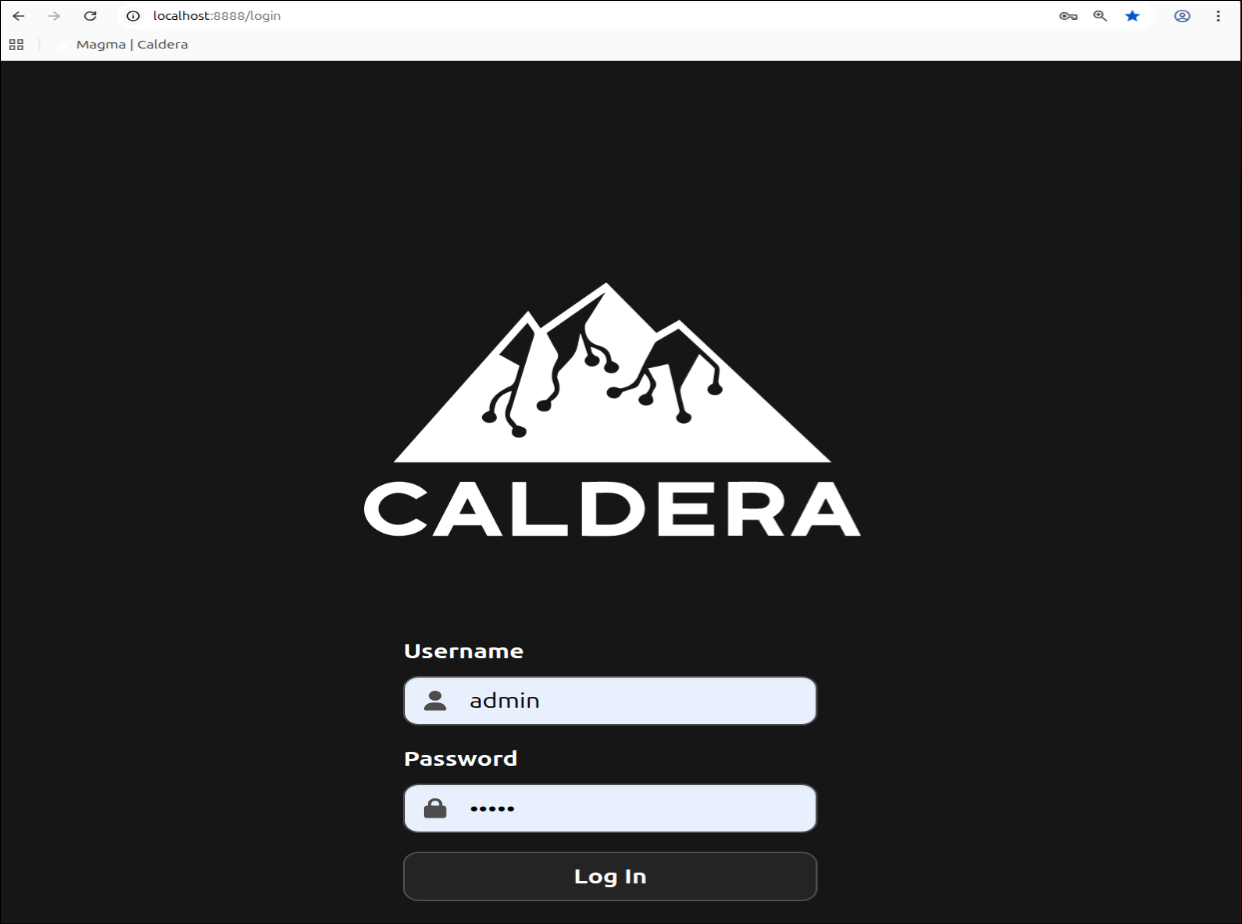
\includegraphics[width=1\textwidth]{figures/caldera_login.png}
        \caption{Caldera administrative login portal.}
        \label{fig:caldera-interface}
    \end{figure}
\end{itemize}

\vspace{1em}
\noindent \textbf{Complexity Metrics Summary:}
\begin{itemize}
    \item \textbf{Total Installation Steps:} 14
    \item \textbf{Total Package Dependencies:} 6
\end{itemize}
        
%% --- SECTION 3: INFECTION MONKEY ---
\subsection{Infection Monkey 's Installation \& Configuration}

The deployment of Infection Monkey focused on establishing the ``Monkey Island'' C2 server. On Ubuntu 24.04, the framework is distributed as an AppImage; however, additional compatibility layers were required to execute the portable binary on a modern kernel.

\begin{itemize}
    \item \textbf{Binary Acquisition and Permissions:} The AppImage (v2.3.0) was retrieved from the official repository. Execution permissions were explicitly granted to the file to allow it to run as a standalone binary.
    
    \begin{lstlisting}[language=bash, caption={Binary Preparation}]
$ chmod u+x InfectionMonkey-v2.3.0.AppImage # Step 1
    \end{lstlisting}

    \item \textbf{Dependency Resolution:} Initial execution attempts failed with a \texttt{dlopen(): error loading libfuse.so.2} error. Modern Ubuntu distributions do not include the FUSE 2 runtime by default, necessitating the installation of the legacy compatibility package.
    
    \begin{lstlisting}[language=bash, caption={Legacy FUSE Support Installation}]
$ sudo apt install libfuse2             # Step 2 [Pkg 1]
    \end{lstlisting}

    \item \textbf{Server Initialization:} The server was manually launched to initialize the Monkey Island backend services. As shown in Figure \ref{fig:monkey-init}, the C2 services successfully started on Port 5000.
    
    \begin{lstlisting}[language=bash, caption={Initial Server Launch}]
$ ./InfectionMonkey-v2.3.0.AppImage     # Step 3
    \end{lstlisting}

    \begin{figure}
        \centering
        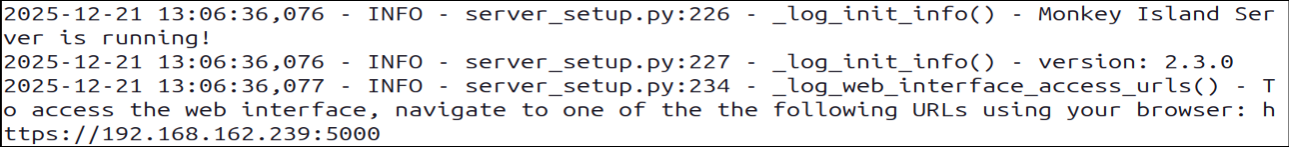
\includegraphics[width=1\textwidth]{figures/monkey_island_logs.png}
        \caption{Terminal output confirming Monkey Island Server is running and accessible via HTTPS.}
        \label{fig:monkey-init}
    \end{figure}

    \item \textbf{Web Interface and Registration:} Upon successful launch, the management console was accessed via a web browser to complete the administrative registration (Figure \ref{fig:monkey-login}).

    \begin{figure}
        \centering
        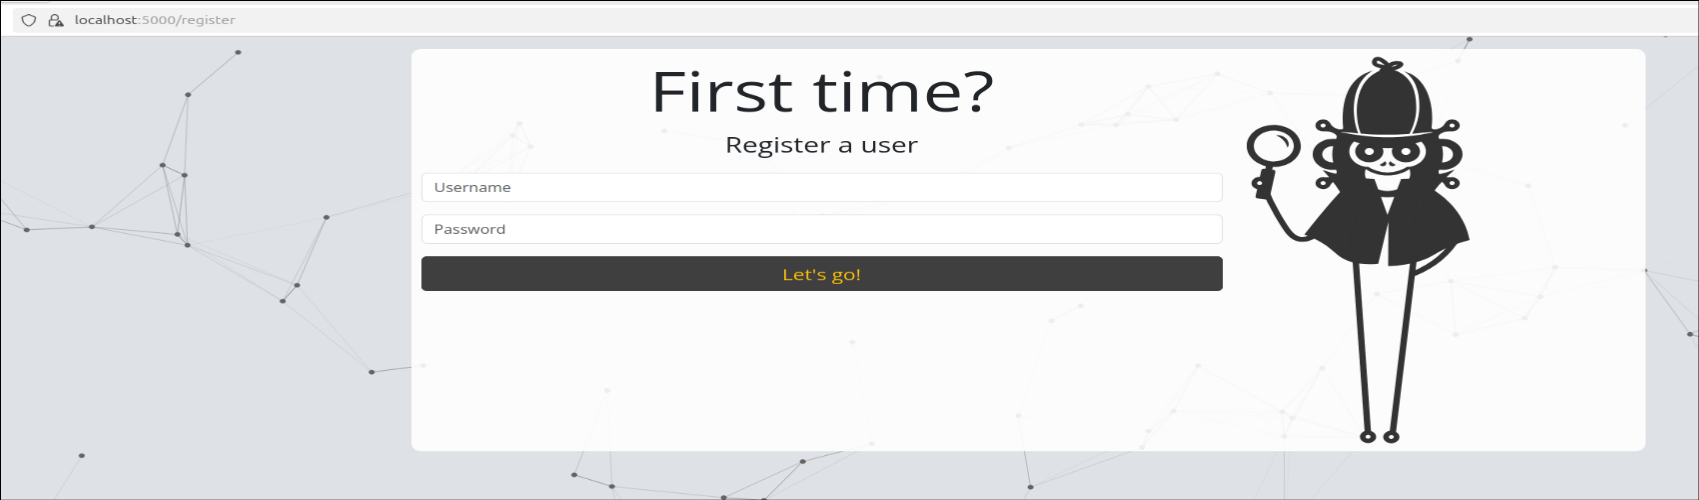
\includegraphics[width=1\textwidth]{figures/monkey_registration.png}
        \caption{Infection Monkey initial user registration interface.}
        \label{fig:monkey-login}
    \end{figure}

    \item \textbf{Persistent Service Configuration:} To ensure the C2 remains active without an open terminal session, the AppImage was registered as a background system service and immediately started.
    
    \begin{lstlisting}[language=bash, caption={System Service Configuration}]
$ ./InfectionMonkey-v2.3.0.AppImage service --install --user bas # Step 4
$ sudo systemctl start infection-monkey # Step 5
    \end{lstlisting}
\end{itemize}

\vspace{1em}
\noindent \textbf{Complexity Metrics Summary:}
\begin{itemize}
    \item \textbf{Total Installation Steps:} 5
    \item \textbf{Total Package Dependencies:} 1
\end{itemize}

%% --- SECTION 4: ATOMIC RED TEAM ---
\subsection{Atomic Red Team 's Installation \& Configuration}

Atomic Red Team provides a library of portable tests mapped to the MITRE ATT\&CK framework. Its execution relies on PowerShell Core, which is not native to Linux and must be installed as a prerequisite.

\begin{itemize}
    \item \textbf{Install PowerShell on Linux:} The installation required registering the proprietary Microsoft package repository before installing the runtime.
    
    \begin{lstlisting}[language=bash, caption={PowerShell Core Installation}]
$ source /etc/os-release
$ wget -q https://packages.microsoft.com/config/ubuntu/$VERSION_ID/packages-microsoft-prod.deb # Step 1
$ sudo dpkg -i packages-microsoft-prod.deb # Step 2
$ sudo apt-get update                   # Step 3
$ sudo apt-get install -y powershell    # Step 4 [Pkg 1]
    \end{lstlisting}

    \item \textbf{Install Execution Framework:} After initializing the PowerShell session, the execution framework and the library of atomic tests (Atomics) were downloaded and installed via the official installation script.
    
    \begin{lstlisting}[language=bash, caption={Framework Installation}]
$ pwsh                                  # Step 5
PS > IEX (IWR 'https://raw.githubusercontent.com/redcanaryco/invoke-atomicredteam/master/install-atomicredteam.ps1' -UseBasicParsing); # Step 6
PS > Install-AtomicRedTeam -getAtomics  # Step 7
    \end{lstlisting}

    As shown in Figure \ref{fig:atomic-success}, the \texttt{Install-AtomicRedTeam} function successfully retrieved the Atomics folder. This process required manual intervention to trust the \textsf{PSGallery} repository.

    \begin{figure}
        \centering
        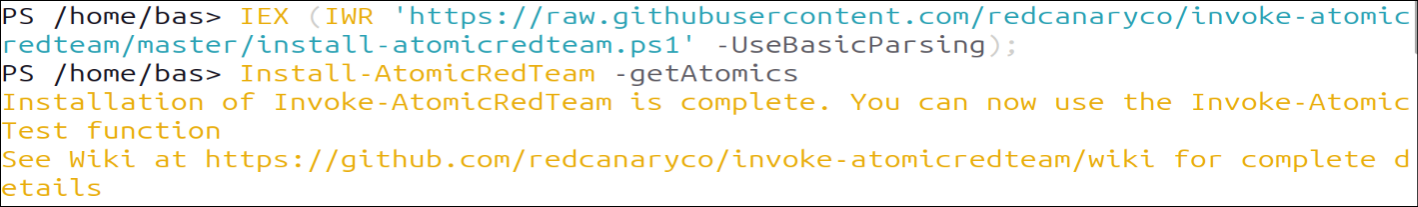
\includegraphics[width=1\textwidth]{figures/atomic-success.png}
        \caption{Output confirming the successful installation of the Atomic Red Team framework and test library.}
        \label{fig:atomic-success}
    \end{figure}

    \item \textbf{Verification:} To confirm operational readiness, the module status was checked to ensure \texttt{Invoke-AtomicRedTeam} was loaded into the session.
    
    \begin{lstlisting}[language=bash, caption={Module Verification}]
PS > Get-Module                         # Step 8
    \end{lstlisting}

    \begin{figure}
        \centering
        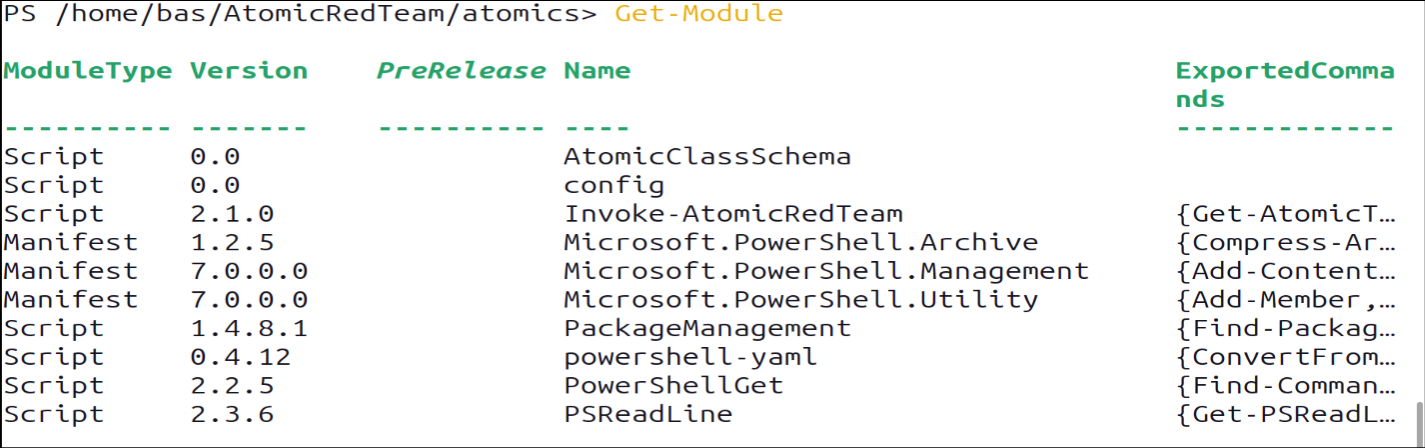
\includegraphics[width=1\textwidth]{figures/atomic-verify.png}
        \caption{Verify the Invoke-AtomicRedTeam module is loaded.}
        \label{fig:atomic-verify}
    \end{figure}
\end{itemize}

\vspace{1em}
\noindent \textbf{Complexity Metrics Summary:}
\begin{itemize}
    \item \textbf{Total Installation Steps:} 8
    \item \textbf{Total Package Dependencies:} 1 (PowerShell Core)
\end{itemize}


%########################################################################%
%#####################|          4.3          |##########################%
%########################################################################%
\section{Attack Simulation Scenarios}\label{sec:AttackScenarios}
To ensure the comparative analysis reflects real-world risk, the attack scenarios for this study were derived using a Threat-Informed Defense approach. We identified high-profile threat actors actively targeting the ASEAN region and global infrastructure in 2025-2026, specifically Mustang Panda\cite{mitre_c0047}\cite{thaicert_mustang}, LockBit\cite{mitre_lockbit}, and Scattered Spider\cite{mitre_c0027}.

To validate the statistical relevance of our selection, we prioritized techniques based on the \textbf{Center for Threat-Informed Defense (CTID) Sightings Ecosystem} (v2.0) \cite{ctid_sightings}. From this global high-prevalence list, we selected 20 specific sub-techniques and adapted them for a \textbf{hybrid multi-victim testbed (Windows and Linux)}, reflecting the cross-platform nature of modern campaigns.

For the purpose of this comparative analysis, these twenty distinct attack simulations are indexed as \textbf{S1} through \textbf{S20} (Scenario 1 to Scenario 20). This indexing system is used throughout the experimental results and the evaluation matrix to facilitate concise cross-referencing. The scenarios are detailed below, categorized by their CTID global prevalence ranking:

% --- RANK 1 ---
\subsection{CTID Rank \#1: Command and Scripting Interpreter (T1059)}
\begin{itemize}
    \item \textbf{S1: PowerShell Execution (Windows)} \\
    \textbf{Technique:} T1059.001 (PowerShell) \\
    \textbf{Origin:} Mustang Panda. \\
    \textbf{Description:} Simulates ``Living-off-the-Land'' by executing Base64-encoded commands directly in memory using \texttt{powershell.exe -enc}, bypassing file-based scanning.

    \item \textbf{S2: Bash Script Execution (Linux)} \\
    \textbf{Technique:} T1059.004 (Unix Shell) \\
    \textbf{Origin:} Mustang Panda (Linux VShell) / LockBit Linux. \\
    \textbf{Description:} Executes a malicious bash script downloaded from a remote source (e.g., \texttt{curl | bash}), a common entry vector for Linux backdoors.
\end{itemize}

% --- RANK 2 ---
\subsection{CTID Rank \#2: Scheduled Task/Job (T1053)}
\begin{itemize}
    \item \textbf{S3: Scheduled Task Creation (Windows)} \\
    \textbf{Technique:} T1053.005 (Scheduled Task) \\
    \textbf{Origin:} LockBit. \\
    \textbf{Description:} Uses \texttt{schtasks.exe} to create a task that runs a payload at system startup, testing persistence detection.

    \item \textbf{S4: Cron Job Persistence (Linux)} \\
    \textbf{Technique:} T1053.003 (Cron) \\
    \textbf{Origin:} LockBit Linux / Scattered Spider. \\
    \textbf{Description:} Appends a malicious entry to the user's crontab (e.g., \texttt{echo "* * * * * /tmp/malware" >> /var/spool/cron/root}) to maintain persistence after reboot.
\end{itemize}

% --- RANK 3 ---
\subsection{CTID Rank \#3: Hijack Execution Flow (T1574)}
\begin{itemize}
    \item \textbf{S5: DLL Side-Loading (Windows)} \\
    \textbf{Technique:} T1574.002 (DLL Side-Loading) \\
    \textbf{Origin:} Mustang Panda (PlugX). \\
    \textbf{Description:} Places a malicious DLL alongside a legitimate, signed executable. When run, the trusted app loads the malware, testing signature-based trust models.
\end{itemize}

% --- RANK 4 ---
\subsection{CTID Rank \#4: Impair Defenses (T1562)}
\begin{itemize}
    \item \textbf{S6: Disable Security Tools (Windows)} \\
    \textbf{Technique:} T1562.001 (Disable Tools) \\
    \textbf{Origin:} LockBit. \\
    \textbf{Description:} Attempts to stop the Windows Defender service (\texttt{Windefend}) or modify registry keys to disable Real-Time Monitoring.

    \item \textbf{S7: Indicator Removal: Clear Logs (Linux)} \\
    \textbf{Technique:} T1070.002 (Clear Linux Logs) \\
    \textbf{Origin:} Scattered Spider. \\
    \textbf{Description:} Deletes critical log files (e.g., \texttt{rm /var/log/auth.log}) and clears shell history (\texttt{history -c}), attempting to blind forensic analysis.
\end{itemize}

% --- RANK 5 ---
\subsection{CTID Rank \#5: Masquerading (T1036)}
\begin{itemize}
    \item \textbf{S8: Match Legitimate Name (Windows)} \\
    \textbf{Technique:} T1036.005 (Match Legitimate Name) \\
    \textbf{Origin:} Mustang Panda (SnakeDisk). \\
    \textbf{Description:} Renames a malicious binary to a system filename (e.g., \texttt{svchost.exe}) and executes it from a temporary folder.

    \item \textbf{S9: Hidden Files and Directories (Linux)} \\
    \textbf{Technique:} T1564.001 (Hidden Files) \\
    \textbf{Origin:} LockBit Linux / General. \\
    \textbf{Description:} Hides a malicious payload by prepending a dot to the filename (e.g., \texttt{/tmp/.malware}), testing if the endpoint sensor monitors hidden artifacts.
\end{itemize}

% --- RANK 10 ---
\subsection{CTID Rank \#10: Remote Services (Lateral Movement) (T1021)}
\begin{itemize}
    \item \textbf{S10: Lateral Movement via SMB (Windows)} \\
    \textbf{Technique:} T1021.002 (SMB/Windows Admin Shares) \\
    \textbf{Origin:} LockBit. \\
    \textbf{Description:} Simulates lateral propagation by connecting to a secondary Windows victim via SMB (Admin Shares) using compromised credentials.

    \item \textbf{S11: SSH Lateral Movement (Linux)} \\
    \textbf{Technique:} T1021.004 (SSH) \\
    \textbf{Origin:} Scattered Spider / LockBit. \\
    \textbf{Description:} Uses a stolen SSH key or credentials to remotely execute commands on a neighboring Linux VM, testing internal network segmentation visibility.
\end{itemize}

% --- RANK 13 ---
\subsection{CTID Rank \#13: Credential Access (T1003)}
\begin{itemize}
    \item \textbf{S12: OS Credential Dumping (Windows)} \\
    \textbf{Technique:} T1003.001 (LSASS Memory) \\
    \textbf{Origin:} Scattered Spider. \\
    \textbf{Description:} Uses \texttt{procdump} to dump the memory of \texttt{lsass.exe}, attempting to harvest NTLM hashes.

    \item \textbf{S13: Credential Dumping: Shadow/SSH (Linux)} \\
    \textbf{Technique:} T1003.008 (Text Files) \\
    \textbf{Origin:} Scattered Spider. \\
    \textbf{Description:} Attempts to read sensitive credential files such as \texttt{/etc/shadow} (password hashes) or \texttt{\textasciitilde/.ssh/id\_rsa} (private keys).
\end{itemize}

% --- RANK 14 ---
\subsection{CTID Rank \#14: System Information Discovery (T1082)}
\begin{itemize}
    \item \textbf{S14: System Discovery (Windows)} \\
    \textbf{Technique:} T1082 (System Info Discovery) \\
    \textbf{Origin:} Mustang Panda. \\
    \textbf{Description:} Runs \texttt{systeminfo} and \texttt{tasklist} to profile the endpoint environment.

    \item \textbf{S15: System Discovery (Linux)} \\
    \textbf{Technique:} T1082 (System Info Discovery) \\
    \textbf{Origin:} LockBit Linux. \\
    \textbf{Description:} Executes enumeration commands like \texttt{uname -a}, \texttt{id}, and \texttt{lscpu} to identify the kernel version and user privileges.
\end{itemize}

% --- RANK 15 ---
\subsection{CTID Rank \#15: Data Encrypted for Impact (T1486)}
\begin{itemize}
    \item \textbf{S16: Bulk File Encryption (Windows)} \\
    \textbf{Technique:} T1486 (Data Encrypted for Impact) \\
    \textbf{Origin:} LockBit 3.0. \\
    \textbf{Description:} Simulates ransomware by rapidly encrypting a folder of documents on Windows using a high-entropy algorithm.

    \item \textbf{S17: Bulk File Encryption (Linux)} \\
    \textbf{Technique:} T1486 (Data Encrypted for Impact) \\
    \textbf{Origin:} LockBit Linux/ESXi Variant. \\
    \textbf{Description:} Simulates the Linux variant of LockBit by encrypting files in the \texttt{/home} directory, testing behavioral detection on Linux.
\end{itemize}

% --- ADDITIONAL ---
\subsection{Additional Cross-Platform Techniques}
\begin{itemize}
    \item \textbf{S18: Ingress Tool Transfer (Mixed)} \\
    \textbf{Technique:} T1105 (Ingress Tool Transfer) \\
    \textbf{Origin:} All Actors. \\
    \textbf{Description:} Downloads a payload using native tools: \texttt{certutil} (Windows) or \texttt{wget/curl} (Linux).

    \item \textbf{S19: SSH Authorized Keys Persistence (Linux)} \\
    \textbf{Technique:} T1098.004 (SSH Authorized Keys) \\
    \textbf{Origin:} Scattered Spider. \\
    \textbf{Description:} Adds a new public key to \texttt{\textasciitilde/.ssh/authorized\_keys} to maintain persistent remote access.

    \item \textbf{S20: Exfiltration Over C2 Channel (Mixed)} \\
    \textbf{Technique:} T1041 (Exfiltration Over C2) \\
    \textbf{Origin:} Mustang Panda. \\
    \textbf{Description:} Simulates data theft by sending dummy data to an external IP via HTTP POST.
\end{itemize}

%######################################################
%########|   List of Selected Attack Simulation Scenarios  |#############
%######################################################
\begin{table}
    \centering
    \caption{List of Selected Attack Simulation Scenarios (Windows \& Linux)}
    \label{tab:attack_scenarios}
    \renewcommand{\arraystretch}{1.2}
    \begin{tabular}{|c|p{3.8cm}|c|c|p{3.5cm}|}
    \hline
    \textbf{ID} & \textbf{Scenario Name} & \textbf{Rank} & \textbf{OS Target} & \textbf{Primary Threat Actor} \\ \hline
    S1 & PowerShell Execution & 1 & Windows & Mustang Panda \\ \hline
    S2 & Bash Script Execution & 1 & Linux & Mustang Panda, LockBit \\ \hline
    S3 & Scheduled Task & 2 & Windows & LockBit \\ \hline
    S4 & Cron Job Persistence & 2 & Linux & LockBit \\ \hline
    S5 & DLL Side-Loading & 3 & Windows & Mustang Panda \\ \hline
    S6 & Disable Security Tools & 4 & Windows & LockBit \\ \hline
    S7 & Clear Logs (History) & 4 & Linux & Scattered Spider \\ \hline
    S8 & Masquerading (Name) & 5 & Windows & Mustang Panda \\ \hline
    S9 & Hidden Files (.file) & 5 & Linux & LockBit \\ \hline
    S10 & SMB Lateral Movement & 10 & Windows & LockBit \\ \hline
    S11 & SSH Lateral Movement & 10 & Linux & Scattered Spider \\ \hline
    S12 & LSASS Dumping & 13 & Windows & Scattered Spider \\ \hline
    S13 & Dump Shadow/Keys & 13 & Linux & Scattered Spider \\ \hline
    S14 & System Discovery & 14 & Windows & Mustang Panda \\ \hline
    S15 & System Discovery & 14 & Linux & LockBit \\ \hline
    S16 & Data Encryption & 15 & Windows & LockBit \\ \hline
    S17 & Data Encryption & 15 & Linux & LockBit \\ \hline
    S18 & Ingress Tool Transfer & - & Mixed & All Actors \\ \hline
    S19 & SSH Key Persistence & - & Linux & Scattered Spider \\ \hline
    S20 & Exfiltration Over C2 & - & Windows \& Linux & Mustang Panda \\ \hline
    \end{tabular}
\end{table}

%================================= Usability & Deployment Complexity

\section{Usability \& Deployment Complexity}\label{sec:Matrix1}
\subsection{Number of installation steps required}\label{sec:Matrix1_1_1}

Deployment friction was quantified by walking each tool's official installation documentation end-to-end and counting every discrete required action (cloning the repository, installing a runtime, running a setup script, editing a configuration file, and starting a service each counted as one step). MITRE Caldera required 14 steps, driven primarily by its Python virtual-environment setup and the need to individually initialize its bundled plugin submodules. Atomic Red Team required 8 steps, centered on its PowerShell installer script and the separate checkout of the atomics test library. Infection Monkey required only 5 steps, reflecting its single self-contained AppImage/Docker distribution model, which collapses most of the setup Caldera and Atomic Red Team require into a single download-and-run action.

\subsection{Dependency requirements}\label{sec:Matrix1_1_2}

Dependency weight was assessed by counting the distinct external runtime packages each tool's own manifest (or documentation) declares as required, excluding vendored or bundled libraries. MITRE Caldera declared 6 packages, reflecting its Python application-server stack and plugin-specific requirements. Infection Monkey and Atomic Red Team each declared a single external dependency --- Infection Monkey ships as a self-contained AppImage/container image, and Atomic Red Team requires only PowerShell 5.1+ (or PowerShell Core), with any additional tooling scoped to individual atomic tests rather than the framework itself.

\begin{table}
    \centering
    \caption{Phase 2 Evaluation: Sub-criterion Scoring Comparison}
    \small
    \begin{tabularx}{\textwidth}{lXXX}
        \toprule
        \textbf{Sub-criterion} & \textbf{MITRE Caldera} & \textbf{Infection Monkey} & \textbf{Atomic Red Team} \\
        \midrule
        1.1 Number of installation steps required & 1 (14 steps) & 3 (5 steps) & 2 (8 steps) \\
        \addlinespace
        1.2 Dependency requirements & 1 (6 packages) & 3 (1 package) & 3 (1 package) \\
        \midrule
        \textbf{Average} & \textbf{1.00} & \textbf{3.00} & \textbf{2.50} \\
        \bottomrule
    \end{tabularx}
\end{table}

Taken together, Infection Monkey presents the lowest deployment barrier of the three tools, while MITRE Caldera's more sophisticated multi-agent, multi-plugin architecture comes at the cost of a heavier and more involved installation process --- a trade-off consistent with prior comparative work on open-source adversary-emulation tooling~\cite{landauer2024}.

%================================= Threat Intelligence Alignment \& Maintenance

\section{Threat Intelligence Alignment \& Maintenance}\label{sec:Matrix2}
\subsection{Frequency of MITRE ATT\&CK techniques update}\label{sec:Update_frequency}

Update frequency was measured via a live pull of each tool's GitHub commit history as of the evaluation date. Atomic Red Team was the most actively updated of the three, with 119 commits in the preceding twelve months (an average of 9.92 per month) and a most recent commit only two days prior to measurement. MITRE Caldera, measured at the ecosystem level (its main repository plus 14 distributed plugin submodules, per the methodological discussion in Section~\ref{sec:Matrix6}), recorded 341 commits over the same period. Infection Monkey recorded zero commits in the preceding twelve months, its last commit dating to 24 July 2024 --- consistent with the project's effective dormancy since release v2.3.0. Both Caldera and Atomic Red Team therefore score [3]~Frequent, while Infection Monkey scores [0]~Static.

\subsection{Update method}\label{sec:Update_method}
A notable framework-level finding for sub-criterion 2.2 is that none of the three evaluated tools provides automated MITRE ATT\&CK content synchronization. The two actively-maintained platforms (MITRE Caldera and Atomic Red Team) both require manual operator intervention --- a \texttt{git pull} or a re-execution of the install script --- to apply new content. Neither offers scheduled background updates, nor immediate synchronization with MITRE's quarterly ATT\&CK release cadence. Infection Monkey lacks any update mechanism beyond replacing the AppImage binary. This represents a categorical gap between open-source and commercial BAS platforms, where automated content synchronization is typically advertised as a key differentiator. The implication for operational deployment is that operators of open-source BAS tooling must establish their own update cadence to ensure ongoing alignment with current threat intelligence.

\begin{table}
    \centering
    \caption{Phase 2 Evaluation: Sub-criterion Scoring Comparison}
    \small
    \begin{tabularx}{\textwidth}{lXXX}
        \toprule
        \textbf{Sub-criterion} & \textbf{MITRE Caldera} & \textbf{Infection Monkey} & \textbf{Atomic Red Team} \\
        \midrule
        2.1 Frequency of MITRE ATT\&CK techniques update & 3 (341/yr\textsuperscript{a}) & 0 (0/yr) & 3 (119/yr) \\
        \addlinespace
        2.2 Update method & 1 (manual git pull) & 0 (no mechanism) & 1 (manual re-install) \\
        \midrule
        \textbf{Average} & \textbf{2.00} & \textbf{0.00} & \textbf{2.00} \\
        \bottomrule
    \end{tabularx}
    \\[4pt]
    \footnotesize\textsuperscript{a}Caldera measured at the ecosystem level (main repository plus 14 plugin submodules); the single-repository count is only 34 commits/yr, which is methodologically misleading for a distributed-plugin architecture (see Section~\ref{sec:Matrix6}).
\end{table}


%========= Scenario Coverage, Reliability & Relevance ===========
\section{Scenario Coverage, Reliability \& Relevance}\label{sec:Matrix3}
\subsection{Number of Supported MITRE ATT\&CK Techniques}\label{sec:results_im_3_1}

This subsection presents the breadth of MITRE ATT\&CK coverage provided by each of the three selected tools as deployed in the laboratory
environment. Coverage was determined by extracting every technique and sub-technique
identifier from each tool's raw ability and configuration files, then cross-referencing each identifier against the official MITRE ATT\&CK Enterprise matrix, version~19.2 (downloaded directly from MITRE on 7 September 2026), which comprises \textbf{697 valid, non-deprecated techniques and sub-techniques} (222 top-level techniques plus 475 sub-techniques) and forms the reference population against which each tool's coverage is assessed in this study. Both parent techniques and their sub-techniques were counted individually
(e.g.\ T1110, T1110.001, T1110.003, and T1110.004 are each recorded as distinct entries), reflecting the granularity at which each tool implements and reports adversarial behaviors. An identifier claimed by a tool but no longer present under that exact identifier in v19.2 --- because MITRE has since deprecated, merged, or renumbered it (for example, the \texttt{T1562} ``Impair Defenses'' family was renumbered to \texttt{T1685} in ATT\&CK~v19) --- was excluded from that tool's count, since it no longer represents a technique the tool can be credited with covering under the current framework.

MITRE Caldera covers 320 of the 697 valid v19.2 techniques (45.9\%), Atomic Red Team covers 317 (45.5\%), and Infection Monkey covers 19 (2.7\%). Both Caldera and Atomic Red Team therefore fall in the [2]~Moderate band (25--50\% coverage), while Infection Monkey falls in the [0]~Minimal band ($<$10\% coverage) --- a consequence of its technique mapping predating ATT\&CK's 2020 sub-technique restructuring and never having been updated to the current identifier scheme.

\subsection{High-Probability Threat Alignment}\label{sec:results_im_3_2}

Whereas Section~\ref{sec:results_im_3_1} measures raw breadth of ATT\&CK coverage, this sub-criterion measures whether each tool covers the 20 high-probability, threat-actor-mapped scenarios (S1--S20, Table~\ref{tab:attack_scenarios}) prioritized for this study from the MITRE Center for Threat-Informed Defense (CTID) top-technique rankings and tied to the Mustang Panda, LockBit, and Scattered Spider TTP profiles introduced in Section~\ref{sec:AttackScenarios}. MITRE Caldera and Atomic Red Team each structurally support 19 of the 20 scenarios (95\%), missing only S5 (T1574.002, DLL Side-Loading), and both therefore score [3]~High Alignment. Infection Monkey supports only 6 of the 20 scenarios (30\%) --- S1, S10, S11, S16, S17, and S18 --- missing every Linux-specific persistence and discovery scenario (S2, S4, S7, S9, S11 excepted, S13, S15), the LSASS credential-dumping scenario (S12), the SSH-key persistence scenario (S19), and the C2-exfiltration scenario (S20). This is a structural scope gap in Infection Monkey's exploiter and post-breach-action library rather than an execution failure, and Infection Monkey therefore scores [1]~Inadequate.

\subsection{Execution reliability}\label{sec:results_im_3_3}

Execution reliability is the primary metric of this study: whether an attempted technique genuinely reached and executed against the intended victim, evidenced by a completion signal specific to each tool's architecture (a full agent round-trip for MITRE Caldera; \texttt{Executing test:} followed by an \texttt{Exit code:} for Atomic Red Team; a technique-specific exploitation or propagation event for Infection Monkey). Reliability was measured across the 19 techniques common to all three tools' campaigns, each run 10 times, for 190 total runs per tool. MITRE Caldera achieved 188/190 successful runs (98.9\%), Atomic Red Team achieved 189/190 (99.5\%), and Infection Monkey achieved 150/190 (78.9\%); all three therefore score [3]~Highly Reliable ($>$75\% success).

Every non-successful run was individually root-caused rather than treated as an undifferentiated failure. MITRE Caldera's two initial non-passing techniques (T1021.002 and T1021.006, lateral movement via SMB and WinRM) were traced to a harness configuration gap --- the CALDERA server lacked a fact source providing the credential and remote-target values its abilities require --- and both reached 10/10 genuine command executions once a proper fact source was supplied, independently confirmed via the victim's own Security and Sysmon event logs. Infection Monkey's non-passing techniques fall into three distinct categories: T1021.001 (RDP) is a confirmed software defect, its RDP exploiter crashing as a subprocess before ever attempting a connection, traced to a PyInstaller frozen-executable interaction with Python's \texttt{spawn} multiprocessing start method; T1003 (OS credential dumping) is a capability-and-environment limitation, since the propagated agent runs without administrative privileges and the target lab has no domain controller for its Zerologon exploiter to target; and detection of T1071.001, although unrelated to execution reliability itself, was separately found to be a fixable Splunk detection-rule defect (the saved search matched on a Sysmon-specific field name that this activity's Security-log events do not populate), corrected during this study.

%%%%%%%%%%%%%%%%%%%%%%%%%%%%%%%%%%%%%%%%%%%%%%%%%%%%%%%%%%%%%%%%%%%%

\section{Operational Performance \& Output Quality}\label{sec:Matrix4}

\subsection{CPU usage of BAS server }\label{sec:Matrix4_4_1}

CPU overhead was measured as each BAS server host's mean CPU utilization during the full campaign's continuous sampling window, expressed as percentage points above that same host's idle baseline. MITRE Caldera showed the smallest overhead of the three tools at +2.83 points, followed by Atomic Red Team at +12.12 points; both fall well within the [3]~Minimal band ($<$15\% overhead). Infection Monkey showed the largest overhead at +18.43 points, placing it in the [2]~Moderate band (15--40\%). A caveat on this comparison is that Atomic Red Team's ``server'' is architecturally a lightweight PowerShell/WinRM command runner on the controller host, whereas MITRE Caldera and Infection Monkey each run a full C2/Island server process; this architectural difference is partly a category distinction rather than a pure measure of code efficiency, and tends to structurally favor Atomic Red Team's figures.

\subsection{Memory usage of BAS server}\label{sec:Matrix4_im_4_2}

Memory overhead was measured using the same continuous-sampling methodology as Section~\ref{sec:Matrix4_4_1}, expressed as percentage points above each host's idle memory baseline. All three tools fall in the [3]~Minimal band ($<$15\% overhead): MITRE Caldera at +1.29 points, Atomic Red Team at +2.48 points, and Infection Monkey at +13.33 points. The same architectural caveat noted for CPU overhead applies here.

\subsection{Quality of reports}\label{sec:Matrix4_4_3}

Report quality was assessed by generating each tool's native output artifact after a completed campaign run and comparing its content against four fixed bands ranging from raw CLI output to specific, actionable remediation guidance. MITRE Caldera produces a structured Operation Report with event logs and named ATT\&CK-technique mitigation guidance, though without machine-actionable detection content such as Snort or Sigma rules, placing it in the [2]~General Advice band. Infection Monkey produces a Security Report with a dedicated ``Machine-related Recommendations'' section offering comparable named mitigation steps, likewise scoring [2]~General Advice. Atomic Red Team emits only raw PowerShell or SSH standard output with no synthesized report file, scoring [0]~No Reports. This result should be read alongside Atomic Red Team's explicit design philosophy as a composable atomic-test executor intended to be wrapped by external tooling (for example, feeding results to a SIEM) rather than to function as a standalone reporting platform; the criterion, as constructed, penalizes this design choice relative to the two all-in-one platforms.

\begin{table}
    \centering
    \caption{Phase 2 Evaluation: Sub-criterion Scoring Comparison}
    \small
    \begin{tabularx}{\textwidth}{lXXX}
        \toprule
        \textbf{Sub-criterion} & \textbf{MITRE Caldera} & \textbf{Infection Monkey} & \textbf{Atomic Red Team} \\
        \midrule
        4.1 CPU usage of BAS server & 3 (+2.83 pts) & 2 (+18.43 pts) & 3 (+12.12 pts) \\
        \addlinespace
        4.2 Memory usage of BAS server & 3 (+1.29 pts) & 3 (+13.33 pts) & 3 (+2.48 pts) \\
        \addlinespace
        4.3 Quality of reports & 2 (mapped mitigations) & 2 (mitigation recs) & 0 (raw stdout only) \\
        \midrule
        \textbf{Average} & \textbf{2.67} & \textbf{2.33} & \textbf{2.00} \\
        \bottomrule
    \end{tabularx}
\end{table}

\section{Framework Extensibility \& Custom Scenario Creation}\label{sec:Matrix5}

\subsection{Add/modify attack scenarios}\label{sec:Matrix5_5_1}

This sub-criterion evaluates the mechanism each tool provides for an operator to add or edit an attack scenario. MITRE Caldera provides both YAML-defined ability files and a dedicated ``Create an Ability'' graphical interface, requiring no programming to author a new scenario, and scores [3]~Easy. Atomic Red Team similarly uses a simple, documented YAML schema per atomic test with no coding required for a standard test, also scoring [3]~Easy. Infection Monkey supports extension only through uploading a compiled plugin package (\texttt{.tar}) via its graphical interface; authoring a new plugin, however, requires Python development against Infection Monkey's plugin architecture, placing it in the [2]~Possible (code required) band.

\subsection{Ease of creating custom TTPs}\label{sec:Matrix5_5_2}

This sub-criterion evaluates how easily an operator can chain multiple techniques into a single coordinated multi-step scenario, distinct from Section~\ref{sec:Matrix5_5_1}'s more basic question of whether a scenario can be authored at all. MITRE Caldera provides Adversary Profiles and Planners that chain individual Abilities into a custom operational sequence entirely through its graphical interface, scoring [3]~User-Friendly. Atomic Red Team's atomics are discrete, single-step tests by design; chaining several into a multi-stage scenario requires external scripting, such as an operator-written PowerShell loop over a sequence of test IDs, placing it in the [2]~Requires Scripting band. Infection Monkey offers no built-in composition mechanism across its fixed exploiter set --- chaining custom multi-stage behavior would require deep changes to its plugin architecture rather than any user-facing configuration --- and it therefore scores [1]~Complex/Undocumented.

\begin{table}
    \centering
    \caption{Phase 2 Evaluation: Sub-criterion Scoring Comparison}
    \small
    \begin{tabularx}{\textwidth}{lXXX}
        \toprule
        \textbf{Sub-criterion} & \textbf{MITRE Caldera} & \textbf{Infection Monkey} & \textbf{Atomic Red Team} \\
        \midrule
        5.1 Add/modify attack scenarios & 3 (YAML + GUI) & 2 (plugin, needs Python) & 3 (YAML, no coding) \\
        \addlinespace
        5.2 Ease of creating custom TTPs & 3 (GUI Planners) & 1 (no composition) & 2 (ext.\ scripting) \\
        \midrule
        \textbf{Average} & \textbf{3.00} & \textbf{1.50} & \textbf{2.50} \\
        \bottomrule
    \end{tabularx}
\end{table}

\section{Community Health \& Project Maturity}\label{sec:Matrix6}

The Criterion~6 measurements reveal a clear three-tier stratification of project 
maturity across the evaluated tools, and confirm one of the central findings 
informing the Phase~1 down-selection in Chapter~3. \textbf{Atomic Red Team} leads on every 
quantitative community metric --- stars (11,895), forks (3,107), all-time 
contributors (498), and active contributors in the past twelve months (35). 
\textbf{MITRE Caldera}, when measured at the ecosystem level (main repository plus the 
14 distributed plugin submodules), records the highest raw commit volume of the 
three tools (341 commits over twelve months versus Atomic Red Team's 185), but with 
a smaller active-contributor pool (21 versus 35). \textbf{Infection Monkey} records 
substantial historical accumulation (6,998 stars and 77 all-time contributors) 
but zero contributors active in the past twelve months and 238 unaddressed open 
issues, consistent with the project's effective dormancy since v2.3.0 in 
September~2023.

The Caldera measurement also illustrates a methodological point worth surfacing 
explicitly. Caldera's main-branch git history shows only 34~commits in the past 
twelve months, none in the past three months --- a pattern that, taken 
in isolation, would suggest project stagnation. The submodule-aware measurement 
reveals the opposite: 175~commits in the past three months alone, distributed 
across the plugin ecosystem, and 12 of 14 plugins updated within the past 
60~days. Single-repository commit counts are not, by themselves, a reliable 
indicator of maintenance pace for projects that follow a distributed plugin 
architecture.
\begin{figure}
    \centering
    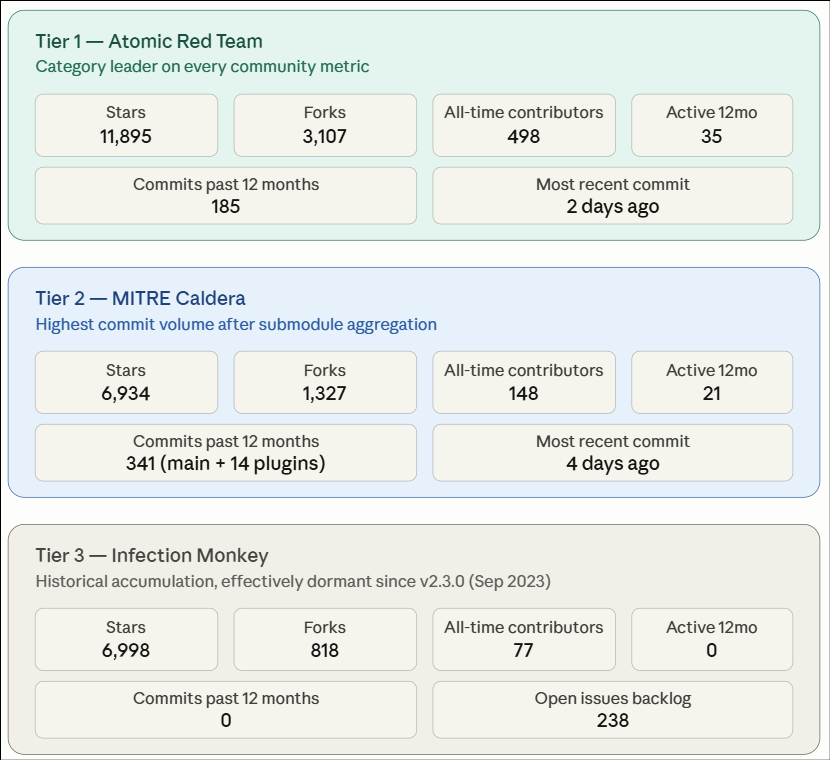
\includegraphics[width=1\linewidth]{figures/Community health and project maturity.png}
    \caption{Community health and project maturity  }
    \label{fig:Community}
\end{figure}

%########################################################################%
%###################|          4.4          |############################%
%########################################################################%

\begin{table}
    \caption{Comparison of breach and attack simulation frameworks}
    \label{tab:results_comparison}
    \centering
    \renewcommand{\arraystretch}{1.3}
    \begin{tabular}{|p{0.50\linewidth}|>{\centering\arraybackslash}p{2cm}|>{\centering\arraybackslash}p{2cm}|>{\centering\arraybackslash}p{2cm}|}
        \hline
        \textbf{Criterion} & \textbf{MITRE Caldera} & \textbf{Infection Monkey} & \textbf{Atomic Red Team} \\ \hline
        
        \multicolumn{4}{|l|}{\textbf{1. Usability \& Deployment Complexity}} \\ \hline
        1.1 Number of installation steps required & 1 \newline \footnotesize{(14)} & 3 \newline \footnotesize{(5)} & 2 \newline \footnotesize{(8)} \\ \hline
        1.2 Dependency requirements & 1 \newline \footnotesize{(6 pkgs)} & 3 \newline \footnotesize{(1 pkg)} & 3 \newline \footnotesize{(1 pkg)} \\ \hline
        \textit{Average} & \textit{1.00} & \textit{3.00} & \textit{2.50} \\ \hline
        
        \multicolumn{4}{|l|}{\textbf{2. Threat Intelligence Alignment \& Maintenance}} \\ \hline
        2.1 Frequency of MITRE ATT\&CK techniques update & 3 \newline \footnotesize{(341/yr\textsuperscript{a})} & 0 \newline \footnotesize{(0/yr)} & 3 \newline \footnotesize{(119/yr)} \\ \hline
        2.2 Update method & 1 \newline \footnotesize{(manual)} & 0 \newline \footnotesize{(none)} & 1 \newline \footnotesize{(manual)} \\ \hline
        \textit{Average} & \textit{2.00} & \textit{0.00} & \textit{2.00} \\ \hline
        
        \multicolumn{4}{|l|}{\textbf{3. Scenario Coverage, Reliability \& Relevance}} \\ \hline
        3.1 Number of supported MITRE ATT\&CK techniques (of 697 valid v19.2 techniques) & 2 \newline \footnotesize{(320/697 = 45.9\%)} & 0 \newline \footnotesize{(19/697 = 2.7\%)} & 2 \newline \footnotesize{(317/697 = 45.5\%)} \\ \hline
        3.2 High-Probability Threat Alignment (CTID top-20) & 3 \newline \footnotesize{(19/20 = 95\%)} & 1 \newline \footnotesize{(6/20 = 30\%)} & 3 \newline \footnotesize{(19/20 = 95\%)} \\ \hline
        3.3 Execution reliability (Attack Rate) & 3 \newline \footnotesize{(98.9\%, 188/190)} & 3 \newline \footnotesize{(78.9\%, 150/190)} & 3 \newline \footnotesize{(99.5\%, 189/190)} \\ \hline
        \textit{Average} & \textit{2.67} & \textit{1.33} & \textit{2.67} \\ \hline

        \multicolumn{4}{|l|}{\textbf{4. Operational Performance \& Output Quality}} \\ \hline
        4.1 CPU usage of BAS server (vs.\ idle baseline) & 3 \newline \footnotesize{(+2.83 pts)} & 2 \newline \footnotesize{(+18.43 pts)} & 3 \newline \footnotesize{(+12.12 pts)} \\ \hline
        4.2 Memory usage of BAS server (vs.\ idle baseline) & 3 \newline \footnotesize{(+1.29 pts)} & 3 \newline \footnotesize{(+13.33 pts)} & 3 \newline \footnotesize{(+2.48 pts)} \\ \hline
        4.3 Quality of reports & 2 \newline \footnotesize{(mapped mitigations)} & 2 \newline \footnotesize{(mitigation recs)} & 0 \newline \footnotesize{(raw stdout only)} \\ \hline
        \textit{Average} & \textit{2.67} & \textit{2.33} & \textit{2.00} \\ \hline

        \multicolumn{4}{|l|}{\textbf{5. Framework Extensibility \& Custom Scenario Creation}} \\ \hline
        5.1 Add/modify attack scenarios & 3 \newline \footnotesize{(YAML + GUI)} & 2 \newline \footnotesize{(plugin, needs Python)} & 3 \newline \footnotesize{(YAML, no coding)} \\ \hline
        5.2 Ease of creating custom TTPs & 3 \newline \footnotesize{(GUI Planners)} & 1 \newline \footnotesize{(no composition)} & 2 \newline \footnotesize{(ext.\ scripting)} \\ \hline
        \textit{Average} & \textit{3.00} & \textit{1.50} & \textit{2.50} \\ \hline

        \multicolumn{4}{|l|}{\textbf{6. Community Health \& Project Maturity}} \\ \hline
        6.1 Frequency of commits/updates & 3 \newline \footnotesize{(341/12mo\textsuperscript{a})} & 0 \newline \footnotesize{(0/12mo)} & 3 \newline \footnotesize{(185/12mo)} \\ \hline
        6.2 Community activity & 2 \newline \footnotesize{(6,934 stars)} & 1 \newline \footnotesize{(6,998 stars)} & 3 \newline \footnotesize{(11,895 stars)} \\ \hline
        \textit{Average} & \textit{2.50} & \textit{0.50} & \textit{3.00} \\ \hline
        \textbf{Overall Average (equal-weighted)} & \textbf{2.36} & \textbf{1.50} & \textbf{2.43} \\ \hline
    \end{tabular}
    \\[4pt]
    \footnotesize\textsuperscript{a}Caldera measured at the ecosystem level (main repository plus 14 plugin submodules); the single-repository count is only 34 commits/12mo, which is methodologically misleading for a distributed-plugin architecture (see Section~\ref{sec:Matrix6}).
\end{table}


%########################################################################%
%###################|          4.5          |############################%
%########################################################################%
\section{Evaluation}\label{sec:Evaluation}

To complement the equal-weighted comparison in Table~\ref{tab:results_comparison}, an Analytic Hierarchy Process (AHP) was applied to derive relative-importance weights for the sub-criteria \emph{within} each of the six evaluation matrices (e.g., within Matrix~4, CPU and Memory overhead were judged equally important and both more important than Report Quality, since resource overhead risks the test environment itself while report quality only affects the follow-up remediation step). Pairwise judgments used Saaty's 1--9 scale, with weights derived via the geometric-mean method and consistency verified via the Consistency Ratio (CR $<$ 0.10 for every matrix).

Deliberately, no cross-matrix weighting was applied to collapse the six matrices into a single overall ranking. Instead, Figure~\ref{fig:spider_chart} visualizes each tool's AHP-weighted score per matrix, so that a reader can identify where each tool is comparatively strong or weak rather than reading a single composite score. MITRE Caldera is weakest on Usability (1.00, reflecting its 14-step install) but strong across the remaining five matrices, particularly Extensibility (3.00). Infection Monkey is strongest on Usability (3.00, the simplest install of the three) but weakest on Threat Intelligence Alignment (0.00, a dormant repository) and Community Health (0.25, dormant despite a historically comparable star count to Caldera). Atomic Red Team is the most balanced of the three tools, with no matrix falling below 2.67 and its strongest showing on Community Health (3.00).

\begin{figure}[h]
\centering
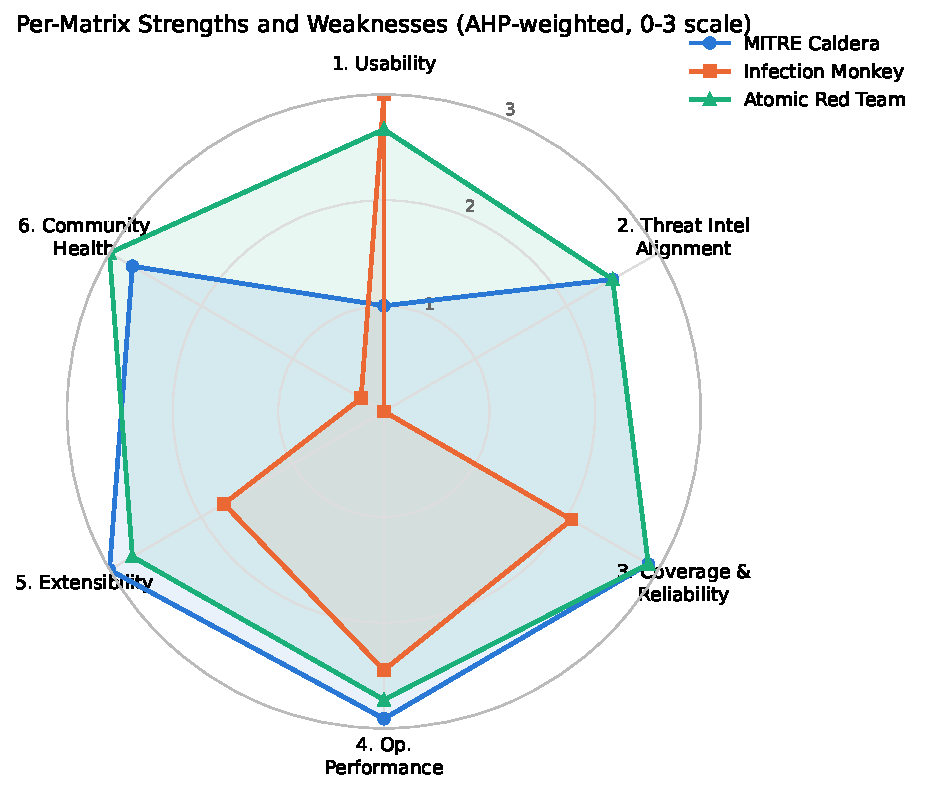
\includegraphics[width=0.75\textwidth]{figures/Figure_4_x_Spider_Chart.pdf}
\caption{Per-matrix strengths and weaknesses of the three BAS frameworks, using AHP-weighted within-matrix sub-criteria scores (0--3 scale). No single overall ranking is asserted: the chart is intended to show each tool's comparative strengths and weaknesses across the six evaluation dimensions rather than to declare one tool categorically ``best.''}
\label{fig:spider_chart}
\end{figure}




















 % Results > EXPERIMENT AND PRELIMINARY RESULTS
%==============================================================================%
%========================|     CHAPTER 5 FUTURE WORK   |=========================%
%==============================================================================%

\chapter{FUTURE WORK} \label{chap:Future}

%###################################################################################%
%##############################|          5.1          |############################%
%###################################################################################%




 % Discussion > FUTURE WORK
%==============================================================================%
%=====================|     CHAPTER 6 CONCLUSION AND RECOMMENDATIONS   |=====================%
%==============================================================================%

\chapter{CONCLUSION AND RECOMMENDATIONS} \label{chap:conclusion}

%###################################################################################%
%##############################|          6.1          |############################%
%###################################################################################%

\section{Conclusion}\label{sec:conclusion}


%###################################################################################%
%##############################|          6.2          |############################%
%###################################################################################%

\section{Recommendations}\label{sec:recommendations}

 % Conclusion and Recommendations

\appendices  % use this if you have more than one appendix
% \appendices resets the `chapter` counter to 0 (muthesis2026.cls), which makes
% hyperref's internal anchor name (\theHchapter, normally == \thechapter) collide
% with Chapter 1's anchor and triggers a "duplicate destination" warning. Give
% appendix chapters their own hyperref-only counter name; the class file is
% left unmodified.
\makeatletter
\renewcommand{\theHchapter}{appendix.\arabic{chapter}}
\makeatother
\chapter{Supplementary Configuration Files}\label{app:configs}
%\section*{hidden appendix section}   %  do not show in table of contents

\chapter{Additional Experimental Results}\label{app:results}
\bibliographystyle{unsrtnat}
\bibliography{references}
\biography % use this to get the biography at the end of the document
\end{document}
